\documentclass[main.tex]{subfiles}
\newcommand\chapterlabel{solids}
\setcounter{figurenewcounter}{0}
\newsavebox\unitcellwater
\newsavebox\trianglenew

\begin{document}
\linenumbers
%\setcounter{chapter}{5}
  

\chapter[Solids and liquids]{Solids and liquids}
%\label{ch:atoms}


      \begin{marginfigure}
      \begin{tikzpicture} \node (a) at (0,0) {\includegraphics[width=4cm]{chapter14/figure1}} node[rotate=90, font=\tiny] at ([yshift=.5cm,xshift=.1cm]a.south east) {\textsuperscript{\textcopyright} PngImg} ;
\end{tikzpicture}
\end{marginfigure}


\lettrine[lines=4]{\color{black!45}T}{here} are three different states of the matter: solid, liquid and gas. At this point, we have studied the properties of gases and liquid solutions. We have not encountered yet solids or pure liquids. This chapter fully deals with the properties of solids and liquids. Liquids have indeed very peculiar properties and this chapter will cover--among other--the vapor pressure. Liquids are not isolated; they are normally in contact with the atmosphere. The liquid molecules which are closer to the air can scape forming a vapor; this vapor exerts certain pressure. This vapor is what you feel, for example, when the weather is very humid. Finally, this chapter covers the idea of intermolecular forces. The molecules of an ideal gas are independent from each other. This means they do not see each other at all--they do not interact with each other. Differently, the molecules of liquids and solids interact with each other by means of stronger force that act between molecules--these are called intermolecular forces. The properties of this forces will help you understand why some liquids boil at higher temperature than others or some solids have higher melting point. 
 
\begin{marginfigure}%LEARNING GOALS BOX
\begin{mytcbox}{GOALS}
\begin{enumerate}[label=\protect\circled{\color{white}\arabic*}]
\item Identify intermolecular forces
\item Identify different types of solids
\item Identify units cells
\item Calculate density of solids
\item Calculate vapor pressure
\end{enumerate}
\end{mytcbox}
\vspace{1cm}
\begin{tcolorbox}[enhanced,colback=red!5!white,colframe=black!50!red,boxrule=1pt,
  arc=0pt,outer arc=0pt,drop heavy lifted shadow]
\faGears\ 
\docenvdef{Discussion:} Do you know other states of the matter other than solid, liquid, or gas?

  \end{tcolorbox}
\end{marginfigure}%LEARNING GOALS BOX



\section{Intermolecular forces}
Atoms in liquid or solid compound are connected by means of chemical bonds, and bonds are forces within molecules. This bonds can be ionic or covalent depending on the nature of the elements that form the molecule. At the same time, the molecules of a liquid or solid compound interact with each other by means of intermolecular forces. The word intermolecular means between molecules. This section describe the three existing types of intermolecular forces as well as its nature and intensity.


\sloppy 
\begin{description}

\item[\docfilehook{Intermolecular forces and intramolecular interactions}{}] Molecules are made of atoms which connect by means of \emph{intra}molecular interactions such as covalent or ionic bonds. Differently, molecules interact with each other by means of \emph{inter}molecular interactions. The prefix \emph{inter} means "occurring between", whereas the prefix \emph{intra} means "occurring within". Intermolecular forces are responsible for the melting and boiling point of a chemical. On one hand, the stronger the forces the higher the melting and boiling point. On the other hand, the more intermolecular interactions the higher the melting and boiling point. This is because in order to melt or boil a chemical we need to overcome the intermolecular forces that connect molecules in order to release the into a different state of matter. In the following we will describe the three main types of intermolecular forces (some books describe four types of intermolecular forces counting the ion-molecule interaction).



\item[\docfilehook{Dispersion forces}{}] All molecules are made of atoms which contain electrons. The electron density of an atom is distributed homogeneously without uneven charge distributions. As a consequence, atoms in general have no permanent dipole moment without negatively or positively charged regions. Still, when two atoms get close together, the presence of each other affects their electron density creating temporary dipole moments. We call this effect polarizability. This temporary dipoles are responsible for London dispersion forces, also called Van der Waals forces or simply dispersion forces.

 \begin{marginfigure}[0cm]
 
   \begin{tikzpicture} \node (a) at (0,0) {\includegraphics[width=4cm, height=4cm,keepaspectratio]{chapter14/figure17}} node[rotate=90, font=\tiny] at ([yshift=.5cm,xshift=.1cm]a.south east) {\textsuperscript{\textcopyright} Flickr} ;
\node[text width=5cm] at ([yshift=0.2cm]a.north) {\mytriangle{red}Polymer molecules interact by means of dispersion};
\end{tikzpicture}
\begin{tikzpicture} \node (a) at (0,0) {\includegraphics[width=8cm, height=4cm,keepaspectratio]{chapter14/figure18}} node[rotate=90, font=\tiny] at ([yshift=.5cm,xshift=.1cm]a.south east) {\textsuperscript{\textcopyright} Flickr} ;
\node[text width=5cm] at ([yshift=0.2cm]a.north) {\mytriangle{red}Fritz London a german physicist is responsible for the name of London forces};
\end{tikzpicture}
\begin{tikzpicture} \node (a) at (0,0) {\includegraphics[width=4cm, height=4cm,keepaspectratio]{chapter14/figure19}} node[rotate=90, font=\tiny] at ([yshift=.5cm,xshift=.1cm]a.south east) {\textsuperscript{\textcopyright} Flickr} ;
\node[text width=5cm] at ([yshift=0.3cm]a.north) {\mytriangle{red}geckos stick because of the van der Waals force};
\end{tikzpicture}

%\caption{Some properties of liquids}
%\label{fig:marginfig2}
\end{marginfigure}





\vspace{-.5cm}
\stepcounter{figurenewcounter}   \refstepcounter{figure}  \label{Fig:{\chapterlabel}\thefigurenewcounter}
     \begin{center}\begin{tikzpicture}
\filldraw[even odd rule,inner color=red,outer color=white, draw=none ] (0,0) circle   (1.0) node [shift={(5em,-4em)}] {\small Unpolarized atoms};
\filldraw[fill=black ] (0,0) circle   (0.1) ;
\filldraw[even odd rule,inner color=red,outer color=white, draw=none ] (3,0) circle   (1.0) ;
\filldraw[fill=black ] (3,0) circle   (0.1) ;

\draw[-{Triangle[width=18pt,length=8pt]}, line width=10pt](4.1,0) -- (5.1, 0);

\begin{scope}[xshift=6.5cm]
\filldraw[even odd rule,inner color=red,outer color=white, draw=none]   (0.00, 0.0) ellipse (0.9 and 1.0) node [shift={(7em,-4em)}] {\small Polarized atoms}   node [shift={(-3em,-0em)}] {\small $\delta -$} node [shift={(3em,-0em)}] {\small $\delta +$};
\filldraw[fill=black ] (0.3,0) circle   (0.1) ;


\filldraw[even odd rule,inner color=red,outer color=white, draw=none]   (4.00, 0.0) ellipse (0.9 and 1.0)   node [shift={(-3em,-0em)}] {\small $\delta +$} node [shift={(3em,-0em)}] {\small $\delta -$} ;
\filldraw[fill=black ] (3.7,0) circle   (0.1) ;
\draw[densely dashdotted] (1.4,0) -- (2.6,0);
\draw [dotted,<-, shift={(0em,1.5em)}] (0,1) -- (1,1) node [shift={(-1em,1em)}] {$d^{\small Temp}$};
\draw [dotted,->, shift={(0em,1.5em)}] (3,1) -- (4,1) node [shift={(-1em,1em)}] {$d^{\small Temp}$};
\node[text width=12cm, fontscale=.3,shift={(-0em,2em)}] at (-3em,-10em) { \begin{bf}\color{black}\bfseries\large Figure \ref{Fig:{\chapterlabel}\thefigurenewcounter} \end{bf} Dispersion forces result from instantaneous dipole moments resulting from the polarization of the electron density of atoms and molecules. };
\end{scope}
\end{tikzpicture}\end{center}
Dispersion forces exist in all chemical, as all chemicals can be polarized. The larger the atomic number, or the molar weight of the compound, the stronger these forces. This is because in general the larger the atomic weight the more polarizable atoms are, and hence, they tend to generate stronger temporary dipoles, produced from charge polarization. \begin{center}
\refstepcounter{table}  \label{tab:{\chapterlabel}1}
\fontfamily{ppl}\selectfont
\begin{tabular}{llll}
\rowcolor{black!45}
\toprule
\multicolumn{4}{l}{\hypersetup{colorlinks,linkcolor={white}} \cellcolor{black}\color{white}\bfseries\small Table \ref{tab:{\chapterlabel}1} Freezing and boiling point of the noble gases } \\
\midrule
 \rowcolor{gray!10} Gas & Atomic Weight (amu) & Melting Point ($^\circ$C) & Boiling Point ($^\circ$C)\\
\midrule
He 	& \multicolumn{1}{c}{2}&\multicolumn{1}{c}{--} &\multicolumn{1}{c}{4} \\ 
Ne 	&  \multicolumn{1}{c}{10}&\multicolumn{1}{c}{25}&	\multicolumn{1}{c}{27 }	\\
Ar 	&  \multicolumn{1}{c}{18}&\multicolumn{1}{c}{84}&	\multicolumn{1}{c}{87} \\
Kr 	&  \multicolumn{1}{c}{36}&\multicolumn{1}{c}{116}&	\multicolumn{1}{c}{121} \\
Xe	&  \multicolumn{1}{c}{54}&\multicolumn{1}{c}{162}&	\multicolumn{1}{c}{167}\\
Rn 	&  \multicolumn{1}{c}{6} &\multicolumn{1}{c}{202} &\multicolumn{1}{c}{211}\\
 \bottomrule
\end{tabular}\end{center} 

The melting (or freezing) and boiling point of the noble gases are given in Table \ref{tab:{\chapterlabel}1}, where you can see how the larger the atomic mass of the gas the higher the melting--and boiling points. Mind that normally, the melting and freezing point of a substance are the same. Dispersion forces are common in chemicals made of hydrogen and carbon--we call these compounds hydrocarbons. The larger the size of the molecule the larger the effects of dispersion forces. For example:
\begin{center}\ce{C6H14} (BP=69$^\circ$C)\hspace{1cm}
\ce{C8H18}(BP=125$^\circ$C)\hspace{1cm}
\ce{C10H22}(BP=174$^\circ$C)\end{center}



\item[\docfilehook{Dipole-Dipole forces}{}] 
Atoms have different electronegativity that is, a different tendency to attract the electron density in a bond. 
In the periodic table, electronegativity increases going from left to right and top to bottom. Elements in the top right of the table (Cl, F) tend to be very electronegative and hence they tend to strongly attract the electrons on a chemical bonds. Differently, elements on the bottom left part of the table are electropositive and they tend to give away the electrons in the bond. Dipole moments result from differences in electronegativity. When a electronegative atoms is connected to a electropositive atom in a bond, the electronegativity difference creates permanent dipole moments and molecules with permanent dipole moment are called polar molecules. The dipole moment of a bond is a vector that points from the most electropositive atom to the most electronegative atom. For example for the O-H and N-H bonds,
\begin{center}\chemfig{
        \chemabove[3pt]{N}{\pol{-} }(-[::270,0.5,,,draw=none]@{a})-
        \chemabove[3pt]{H}{\pol{+}}(-[::270,0.5,,,draw=none]@{b})
        }
\chemmove{
          \draw[|->, very thick] (b)--(a);
         } 
\qquad
\chemfig{
         \chemabove[3pt]{H}{ \pol{+}}(-[::270,0.5,,,draw=none]@{c})-
         \chemabove[3pt]{O}{ \pol{-}}(-[::270,0.5,,,draw=none]@{d})
        }
\chemmove{
          \draw[|->, very thick] (c)--(d);
          }
\end{center}
As such, the molecule \ce{HCl} would be polar as results from the combination of a electropositive atom (H) and an electronegative atom (Cl). Similarly, \ce{HF} would be a polar molecule too. Dipole-dipole forces exist only in polar compounds, being the result of permanent dipole moments.  This types of interactions are stronger that dispersion forces but weaker than normal interatomic covalent bonds. Molecules with dipole moment can attract each other by means of dipole forces, orienting themselves so that their positive side aligns with the negative side maximizing the electrostatic attraction. At the same type, dipole forces depend on the distance and at large distance are less effective.


\newcommand{\Bond}[6]%
% start, end, thickness, incolor, outcolor, iterations
{ \begin{pgfonlayer}{background}
        \colorlet{InColor}{#4}
        \colorlet{OutColor}{#5}
        \foreach \I in {#6,...,1}
        {   \pgfmathsetlengthmacro{\r}{#3/#6*\I}
            \pgfmathsetmacro{\C}{sqrt(1-\r*\r/#3/#3)*100}
            \draw[InColor!\C!OutColor, line width=\r] (#1.center) -- (#2.center);
        }
    \end{pgfonlayer}
}

\newcommand{\SingleBond}[2]%
% start, end
{   \Bond{#1}{#2}{1mm}{white}{gray!50}{10}
}

 
 \vspace{1cm}


\stepcounter{figurenewcounter}   \refstepcounter{figure}  \label{Fig:{\chapterlabel}\thefigurenewcounter}
     \begin{center}\begin{tikzpicture}
     [   oxygen/.style={circle, ball color=red, minimum size=6mm, inner sep=0},
    hydrogen/.style={circle, ball color=white, minimum size=2.5mm, inner sep=0},
    carbon/.style={circle, ball color=black!75, minimum size=7mm, inner sep=0}
]
 \begin{scope}  [transform canvas={rotate=-0, shift={(-25em,0em)}}]

     \fill [left color=blue!60!black, right color=yellow!85!black] (0,0) ellipse (2em and .9em) node[text=blue,shift={(1.5em,0em)}] {\small $\delta ^+$} node[text=white,shift={(-1em,0em)}] {\small $\delta^-$};
\draw [blue,thick,<-, shift={(-0.5em,0.6em)}] (-1.5em,0.5em) -- (2em,0.5em) node [shift={(-1em,1em)}] {$d$};
\begin{scope}[shift={(7em,0em)}]
\fill [left color=blue!60!black, right color=yellow!85!black] (0,0) ellipse (2em and .9em) node[text=blue,shift={(1.5em,0em)}] {\small $\delta ^+$} node[text=white,shift={(-1em,0em)}] {\small $\delta^-$};
\draw [blue,thick,<-, shift={(-0.5em,0.6em)}] (-1.5em,0.5em) -- (2em,0.5em) node [shift={(-1em,1em)}] {$d$};
\end{scope}
\draw[densely dashdotted] (0.7,0) -- (2.,0);
 \end{scope}
 
 \draw[densely dashdotted] (-2,-0.2) -- (-0.2,-0.3);

 \begin{scope}  [transform canvas={rotate=-45, shift={(-5em,-5em)}}]
   \node[rotate=45, shift={(-0.4em,1.5em)}]  (0,0) { \chemfig{\origorbital[half ]{p}}};
   \node[rotate=-45, shift={(0.4em,1.5em)}]  (0,0) { \chemfig{\origorbital[half ]{p}}};
  \node[oxygen] (O1) at (0,0) {};
    \node[hydrogen] (H1) at (1,-0.5) {};
    \node[hydrogen] (H2) at (-1,-0.5) {};
         \SingleBond{[rotate=-45, shift={(-5em,-5em)}]O1}{[rotate=-45, shift={(-5em,-5em)}]H1}
    \SingleBond{[rotate=-45, shift={(-5em,-5em)}]O1}{[rotate=-45, shift={(-5em,-5em)}]H2}    \end{scope}
    
    \def\xwater{-2}
        \def\ywater{-2}
      \begin{scope}  [transform canvas={rotate=-155, shift={(\xwater em,-\ywater em)}}]
   \node[rotate=45, shift={(-0.4em,1.5em)}]  (0,0) { \chemfig{\origorbital[half ]{p}}};
   \node[rotate=-45, shift={(0.4em,1.5em)}]  (0,0) { \chemfig{\origorbital[half ]{p}}};
  \node[oxygen] (O1) at (0,0) {};
    \node[hydrogen] (H1) at (1,-0.5) {};
    \node[hydrogen] (H2) at (-1,-0.5) {};
        \SingleBond{[rotate=-155, shift={(\xwater em,-\ywater em)}]O1}{[rotate=-155, shift={(\xwater em,-\ywater em)}]H1}
    \SingleBond{[rotate=-155, shift={(\xwater em,-\ywater em)}]O1}{[rotate=-155, shift={(\xwater em,-\ywater em)}]H2}    \end{scope}

%       
%        \begin{scope}  [transform canvas={rotate=-45, shift={(-10 em,-5em)}}]
%   \node[rotate=45, shift={(-0.4em,1.5em)}]  (0,0) { \chemfig{\origorbital[half ]{p}}};
%   \node[rotate=-45, shift={(0.4em,1.5em)}]  (0,0) { \chemfig{\origorbital[half ]{p}}};
%  \node[oxygen] (O1) at (0,0) {};
%    \node[hydrogen] (H1) at (1,-0.5) {};
%    \node[hydrogen] (H2) at (-1,-0.5) {};
%       \SingleBond{[rotate=-45, shift={(-10 em,-5em)}]O1}{[rotate=-45, shift={(-10 em,-5em)}]H1}
%    \SingleBond{[rotate=-45, shift={(-10 em,-5em)}]O1}{[rotate=-45, shift={(-10 em,-5em)}]H2}    \end{scope}
       
\node[text width=12cm, fontscale=.2,shift={(-8em,-12em)}] at (-1em,5em) { \begin{bf}\color{black}\bfseries\large Figure \ref{Fig:{\chapterlabel}\thefigurenewcounter} \end{bf} (Left) Dipole-dipole forces result from the interaction of permanent dipole moments existing in polar molecules. (Right) two water molecules interacting by means of hydrogen bonds };


\end{tikzpicture}\end{center}

The dipole moment of a molecule is measured in Debye (D). For example, the dipole moment of \ce{HCl} is 1.05D, whereas the dipole moment of \ce{HF} is 1.82D. The stronger the dipole moment the stronger the dipole-dipole interactions. For example, when comparing \ce{C3H8} and \ce{CH3OCH3}, the former has a almost null dipole moment, whereas the later has a dipole moment of 1.3D. The boiling point of  \ce{C3H8} is -42$^\circ$C whereas the boiling point of \ce{CH3OCH3} is -25$^\circ$C. The table below list some dipole moments and boiling points showing the trend that the larger the dipole moment the higher (more positive) the boiling point.

 

\refstepcounter{table}  \label{tab:{\chapterlabel}2}
\fontfamily{ppl}\selectfont
\begin{center}\begin{tabular}{lll}
\rowcolor{black!45}
\toprule
\multicolumn{3}{l}{\hypersetup{colorlinks,linkcolor={white}} \cellcolor{black}\color{white}\bfseries\small Table \ref{tab:{\chapterlabel}2} Boiling (BP) point of a series of hydroacids } \\
\midrule
 \rowcolor{gray!10} Compound & Dipole moment (Debyes) &  Boiling Point ($^\circ$C)\\
\midrule
\ce{C3H8} 	& \multicolumn{1}{c}{0.1} &		\multicolumn{1}{c}{-42}  \\ 
\ce{CH3OCH3} 	&  \multicolumn{1}{c}{1.3} &	\multicolumn{1}{c}{-25} 	\\
\ce{CH3Cl} 	&  \multicolumn{1}{c}{2.0} &	\multicolumn{1}{c}{-24} 	\\
\ce{CH3COH}  	&  \multicolumn{1}{c}{2.7} &	\multicolumn{1}{c}{-21} \\
\ce{CH3CN}	&  \multicolumn{1}{c}{3.9}&\multicolumn{1}{c}{	-82}  \\
 \bottomrule
\end{tabular}\end{center}




\item[\docfilehook{Hydrogen bonds }{}] Hydrogen bonds are the strongest of all intermolecular forces and exist only in molecules containing very specific bonds; in particular they only exist in molecules containing \ce{H-F}, \ce{H-N} or \ce{H-O} bonds. An example of molecule with hydrogen bonds are \ce{HF} or \ce{NH3}. Hydrogen bonds are a specific type dipole-dipole interactions responsible, among other, for some of the high boiling point of water. Due to the existence of hydrogen bonds water is liquid at room temperature (\ce{H2O}, BP=100$^\circ$C), in comparison with similar molecules (\ce{H2S}, BP=-60$^\circ$C). The anomalous character of oxygen, fluorine and nitrogen results from the fact that these are very electronegative elements with  lone pairs of electrons--these are non-bonding pairs of electrons--that enable the creation of hydrogen bonds. In particular, oxygen has two lone pairs, nitrogen one and fluorine three. The combination of high electronegativity, the presence of lone pairs and the presence of hydrogen atoms, makes hydrogen bond possible.








\begin{example} %%%%%%%%%%%%%%%%%%%%%%%% EXAMPLE BOX
Indicate what types of intermolecular forces exist in the following molecules:\\
\begin{tabularx}{\textwidth}{
    >{\centering}m{.185\linewidth} 
    *{4}{Y} }
  \toprule
 & \ce{HCl}  &  \ce{CH4}  &\ce{H2O} & \ce{CH3Cl}   \\
    \midrule
   Dispersion & 	 &		 &    &		   \\
  Dipole-Dipole& 	 &		&     &		     \\
      H-bonds & 	 &		 &    &		\\    
    \bottomrule
\end{tabularx}
\\
\textlcsc{ \textcolor{dgreen}{\Large \textbf{Solution}} }\\
All molecules can interact by means of dispersion forces. Differently, only polar molecules can interact by means of dipole-dipole forces. Finally, only molecules with a  \ce{H-F}, \ce{H-N} or \ce{H-O} bond can interact by means of hydrogen bonds. For these reason, from the table only \ce{HCl},  \ce{H2O} and \ce{CH3Cl} has dipole forces, and only \ce{H2O} has hydrogen bonds.
\begin{tabularx}{\textwidth}{
    >{\centering}m{.185\linewidth} 
    *{4}{Y} }
  \toprule
 & \ce{HCl}  &  \ce{CH4}  &\ce{H2O} & \ce{CH3Cl}   \\
    \midrule
   Dispersion & 	\checkmark &	\checkmark	 & \checkmark   &\checkmark		   \\
  Dipole-Dipole&  \checkmark	 &	\xmark 	& \checkmark    &\checkmark		     \\
      H-bonds & 	\xmark  &\xmark 		 &\checkmark    &\xmark 		\\    
    \bottomrule
\end{tabularx}
\\
\faDiamond\ \textlcsc{ \textcolor{dgreen}{\Large \textbf{Study Check}} }\\
Indicate what types of intermolecular forces exist in the following molecules: \ce{NH_3}, \ce{HF}, and \ce{CH_3-CH_3}.
\begin{flushright} Answer: all have dispersion, only \ce{NH_3}, \ce{HF} has dipole and only \ce{NH_3}, \ce{HF} has H-bonds.\end{flushright}
\end{example}%%%%%%%%%%%%%%%%%%%%%%%% EXAMPLE BOX



\item[\docfilehook{Intermolecular forces of liquids and boiling  }{}] Boiling a liquid requires energy. This energy is invested in separating the molecules from the liquid until they are spread apart. In order to separate the molecules of a liquid, we need to overcome intermolecular forces. Imagine boiling \ce{CH4}. We know the molecules of methane only interact among themselves by means of weak dispersion forces. Imagine now boiling water. Water is polar and water has \ce{O-H} bonds, hence water molecules interact by means of dispersion, dipole-dipole and hydrogen bonds. The energy needed to separate the molecules of water will be larger than the energy required to separate the molecules of methane. The more intense the intermolecular forces, the higher the boiling point. Also, the more types of intermolecular forces present in a liquid the higher the boiling point. Finally, we can apply these ideas not only to liquids but also to solids.
\begin{example} %%%%%%%%%%%%%%%%%%%%%%%% EXAMPLE BOX
Compare the boiling point of these two molecules: \ce{HCl} and \ce{H2O}.
\\
\textlcsc{ \textcolor{dgreen}{\Large \textbf{Solution}} }\\
Let us build a table with the different types of intermolecular forces present in each liquid. The molecules of both liquids can interact by means of dispersion forces and also dipole-dipole forces, as both are polar molecules. Differently, only molecules with a  \ce{H-F}, \ce{H-N} or \ce{H-O} bond can interact by means of hydrogen bonds. For these reason,  \ce{H2O} liquid contains  hydrogen bonds.\\
\begin{tabularx}{\textwidth}{
    >{\centering}m{.185\linewidth} 
    *{2}{Y} }
  \toprule
 & \ce{HCl}    &\ce{H2O}    \\
    \midrule
   Dispersion & 	\checkmark &	\checkmark	  		   \\
  D-D&  \checkmark	 &	\checkmark	 	     \\
      H-bonds & 	\xmark  &\checkmark 		   		\\    
    \bottomrule
\end{tabularx}
Hence, water will boil at a higher temperature.
\\
\faDiamond\ \textlcsc{ \textcolor{dgreen}{\Large \textbf{Study Check}} }\\
Compare the boiling point of these two molecules: \ce{CH3F} and \ce{CH4}.
\begin{flushright} Answer: BP(\ce{CH3F})>BP(\ce{CH4}).\end{flushright}
\end{example}%%%%%%%%%%%%%%%%%%%%%%%% EXAMPLE BOX
\end{description}

\newpage
\section{The solid state}
What makes solids unique in comparison to liquids and gases? They answer is their structure. There are two main different types of solids: crystalline solids and amorphous solids. Crystalline solids are made of atoms or molecules periodically, regularly, arranged in the three dimensions of the space. Examples of a crystalline solid are table salt or sugar. Amorphous solids have disordered structures. An example of an amorphous solid is window glass. This section will focus on the properties of crystalline solids as their periodicity makes their properties easier to study.
%\begin{marginfigure}
%      \includegraphics{chapter14/figure2}   \vspace{1cm}
%            \includegraphics{chapter14/figure3}      
%      \caption{Cooking salt, \ce{NaCl} is a crystalline solid, whereas glass, \ce{SiO2} is an amorphous solid.}
%   \end{marginfigure}
\sloppy 
\begin{description}




\item[\docfilehook{Crystalline lattice: the unit cell}{}] The structure of crystalline solids is periodic. The term does not refer to periodic in time, but in periodic in space. Hence, the structure of crystalline solids is the result of the repetition of a small piece of the structure in the space. The overall structure is called \emph{crystalline lattice}. Here an example of a very simple two dimensional lattice. In this lattice, the central box is repeated infinitely in two directions of the space generating a lattice.\vspace{-1cm}
\stepcounter{figurenewcounter}   \refstepcounter{figure}  \label{Fig:{\chapterlabel}\thefigurenewcounter}
     \begin{center}
% You can tweak these
\colorlet{odd plane}{black!20}
\colorlet{even plane}{black!20}
\def\ballradius{0.45}


\def\DrawRow#1#2{
    \foreach \x in {0,...,#2}
       \shade[ball color=ball] ($(#1) +(\x, 0,0)$) circle(\ballradius);
}
\def\DrawOddPlane#1{ 
  \pgfmathsetmacro{\aux}{#1-1}
  \colorlet{ball}{odd plane}
  \foreach \z in {0,...,#1} {
      \DrawRow{0,0,\z}{#1}
      \if\z#1\relax\else
      \DrawRow{0.5,0,\z+0.5}{\aux}
      \fi
  }
}
\def\DrawEvenPlane#1{ 
  \pgfmathsetmacro{\aux}{#1-1}
  \colorlet{ball}{even plane}
  \foreach \z in {0,...,#1} {
      \DrawRow{0.5,0,\z}{\aux}
      \if\z#1\relax\else
      \DrawRow{0,0,\z+0.5}{#1}
      \fi
  }
}

\begin{tikzpicture}
   \foreach \y in {0,...,3} {
      \begin{scope}[yshift=\y cm]
          \DrawOddPlane{3}
      \end{scope}
      \if\y3\relax\else
      \begin{scope}[yshift=\y cm + 0.5cm]
          \DrawEvenPlane{3}
      \end{scope}
      \fi
  }
    \pgfmathsetmacro{\cubex}{1}
    \pgfmathsetmacro{\cubey}{1}
    \pgfmathsetmacro{\cubez}{1}
    \draw (3,3,3) -- ++(-\cubex,0,0) -- ++(0,-\cubey,0) -- ++(\cubex,0,0) -- cycle;
    \draw (3,3,3) -- ++(0,0,-\cubez) -- ++(0,-\cubey,0) -- ++(0,0,\cubez) -- cycle;
    \draw (3,3,3) -- ++(-\cubex,0,0) -- ++(0,0,-\cubez) -- ++(\cubex,0,0) -- cycle;

%%%%%%%%%%%%%%%%%%%%%%%%%%%%
\coordinate (spy point) at (6em,3em);
\coordinate (magnifying glass) at (17em,-0em);
\node [draw=none, shape=circle, inner sep=3.5em, postaction={decorate,decoration={raise=-0.6em, text along path,text align=right,text={|\tiny\color{black}|{\textsuperscript{\textcopyright}} Wikipedia}}}]  (a) at (magnifying glass) {};
\draw[draw=none, fill=gray, fill opacity=0.2] (spy point) to [bend left=-45] (a.south) -- (a.west)  to [bend right=-45]  (spy point) -- cycle;
\node  [thin, draw=black, shape=circle, inner sep=3.5em, fill overzoom image=chapter14/figure20]  (c) at (magnifying glass) {} node[yshift=0.5em] at (c.north) {crystalline solid};
%%%%%%%%%%%%%%%%%%%%%%%%%%%%

\node[text width=12cm, fontscale=.6] at (5em,-7em) { \begin{bf}\color{black}\bfseries\large Figure \ref{Fig:{\chapterlabel}\thefigurenewcounter} \end{bf} Unit cell of a solid of a crystalline solid. The whole structure of the solid results from the replication of a unit cell and just this unit cell is necessary to characterize the structure of the solid. };
  
\end{tikzpicture}\end{center}




As the lattice is made of repetition, the smallest repeating unit is called the \emph{unit cell}. Therefore, simply with the unit cell one can generate the whole crystal lattice by repeating the unit cell in the tree dimensions. Therefore, it is unnecessary to study the crystalline whole lattice  as the unit cell is enough to understand many properties of crystalline solids such as their density. In the following we will study in more detail the properties of crystalline solids and some of the most common unit cells.
\item[\docfilehook{Types of crystalline solids}{}] Examples of crystalline solids are: sugar and table salt. These two solids have very different constitutions. Table salt is made of ions: \ce{Na+} and \ce{Cl-}. Sugar is made of molecules. We say \ce{NaCl} is an ionic solid, whereas sugar is a \emph{molecular solid}. Other examples of \emph{ionic solids}: \ce{MgO}, \ce{CaF2}. Other examples of \emph{molecular solids}: ice which is made of water molecules. A third type of crystalline solids are called \emph{atomic solids}, as they are made of atoms. Think of metallic iron or graphite. Both are atomic solids made of atoms, \ce{Fe} and \ce{C}. Overall, molecular solids are made or molecules--often times covalent molecules--whereas ionic solids are made of ions and result from ionic compounds. Finally, atomic solids are made of atoms. In the following we will study more about a specific type of atomic solids: metallic solids. Metallic solids are indeed atomic solids made of metallic elements, such as for example gold (\ce{Au_{(s)}}).
\stepcounter{figurenewcounter}   \refstepcounter{figure}  \label{Fig:{\chapterlabel}\thefigurenewcounter}
    
    \hspace{-2cm}\begin{minipage}[b]{1.5\linewidth}


  
     \savebox\unitcellwater{ 
     \begin{tikzpicture}\path (0.45,3.3) node {\includegraphics[width=0.75cm]{chapter14/water}}
      (1.6,4.4)  node {\includegraphics[width=0.75cm]{chapter14/water}}
      (0.5,4.45) node {\includegraphics[width=0.75cm]{chapter14/water}}
      (1.1,3.7)  node {\includegraphics[width=0.75cm]{chapter14/water}};
 \path[draw,ultra thick] (0,3) rectangle (2,5);\end{tikzpicture}}
    \begin{center}
\begin{tikzpicture}

\begin{scope}[every node/.append style={transform shape}, shift={(-15em,0)}, scale=0.9]
\begin{scope}[shift={(-4,0)}]
\foreach \x in {5,7,9} {
    \foreach \y in {1,3,5} {
        % water molecules in images
        \node at (\x+0.45,\y+0.3)         {\includegraphics[width=0.75cm]{chapter14/water}};
       \node at (\x+1.6 ,\y+1.4) {\includegraphics[width=0.75cm]{chapter14/water}};
        \node at (\x+0.5 ,\y+1.45) {\includegraphics[width=0.75cm]{chapter14/water}};
        \node at (\x+1.1 ,\y+0.7) {\includegraphics[width=0.75cm]{chapter14/water}};
        % edge of each box
     }
}\end{scope}
\begin{scope}[shift={(4,0)}]

% periodic boundaries
\foreach \x in {5,7,9} {
    \foreach \y in {1,3,5} {
        % water molecules in images
        \node at (\x+0.45,\y+0.3)         {\includegraphics[width=0.75cm]{chapter14/water}};
       \node at (\x+1.6 ,\y+1.4) {\includegraphics[width=0.75cm]{chapter14/water}};
        \node at (\x+0.5 ,\y+1.45) {\includegraphics[width=0.75cm]{chapter14/water}};
        \node at (\x+1.1 ,\y+0.7) {\includegraphics[width=0.75cm]{chapter14/water}};
        % edge of each box
        \path[draw,thick] (\x,\y) rectangle (\x+2,\y+2);
    }
}
% central box thicker than other
\path[draw,ultra thick] (7,3) rectangle (9,5);
% an arrow
\path[draw,ultra thick,->] (2.5,4) -- (4.5,4);
% dashed lines 
\foreach \x in {5,7,9,11} {
    % vertical
    \path[draw,dashed,thick] (\x,0) -- (\x,1) (\x,7) -- (\x,8);
    % horizontal
    \path[draw,dashed,thick] (4,\x-4) -- (5,\x-4) (11,\x-4) -- (12,\x-4);
}
\end{scope}
\end{scope}
%%%%%%%%%%%%%%%%%%%%%%%%%%%%
\coordinate (spy point) at (12em,6em);
\coordinate (magnifying glass) at (30em,10em);
\node [draw=none, shape=rectangle, inner sep=2.5em, postaction={decorate,decoration={raise=-0.6em, text along path,text align=right   }}]  (a) at (magnifying glass) {};
\draw[draw=none, fill=gray, fill opacity=0.2] (spy point) to [bend left=-45] ([shift={(-0,0)}]a.north west) -- (a.south west)  to [bend right=-45]  (spy point) -- cycle;
 \node  [thin, draw=none, shape=rectangle, inner sep=2.5em]  (c) at (magnifying glass) {\usebox\unitcellwater} node[yshift=-0.5em] at (c.north) {Unit cell};
%\node  [thin, draw=black, shape=circle, inner sep=3.5em, fill overzoom image={\usebox\unitcellwater}]  (c) at (magnifying glass) { } node[yshift=0.5em] at (c.north) {crystalline solid};
%%%%%%%%%%%%%%%%%%%%%%%%%%%%
\node[text width=12cm, fontscale=.8, shift={(4em,-1em)}] at (0em,-0em) { \begin{bf}\color{black}\bfseries\large Figure \ref{Fig:{\chapterlabel}\thefigurenewcounter} \end{bf} A periodic structure made of water molecules. The unit cell on the left contains four water molecules. The repetition of the unit cell, on the right, generates a two-dimensional structure. };
  
\end{tikzpicture}\end{center}\end{minipage}



%\begin{marginfigure}
%      \includegraphics{chapter14/figure4}   \vspace{1cm}
%            \includegraphics{chapter14/figure5}   \vspace{1cm}   
%      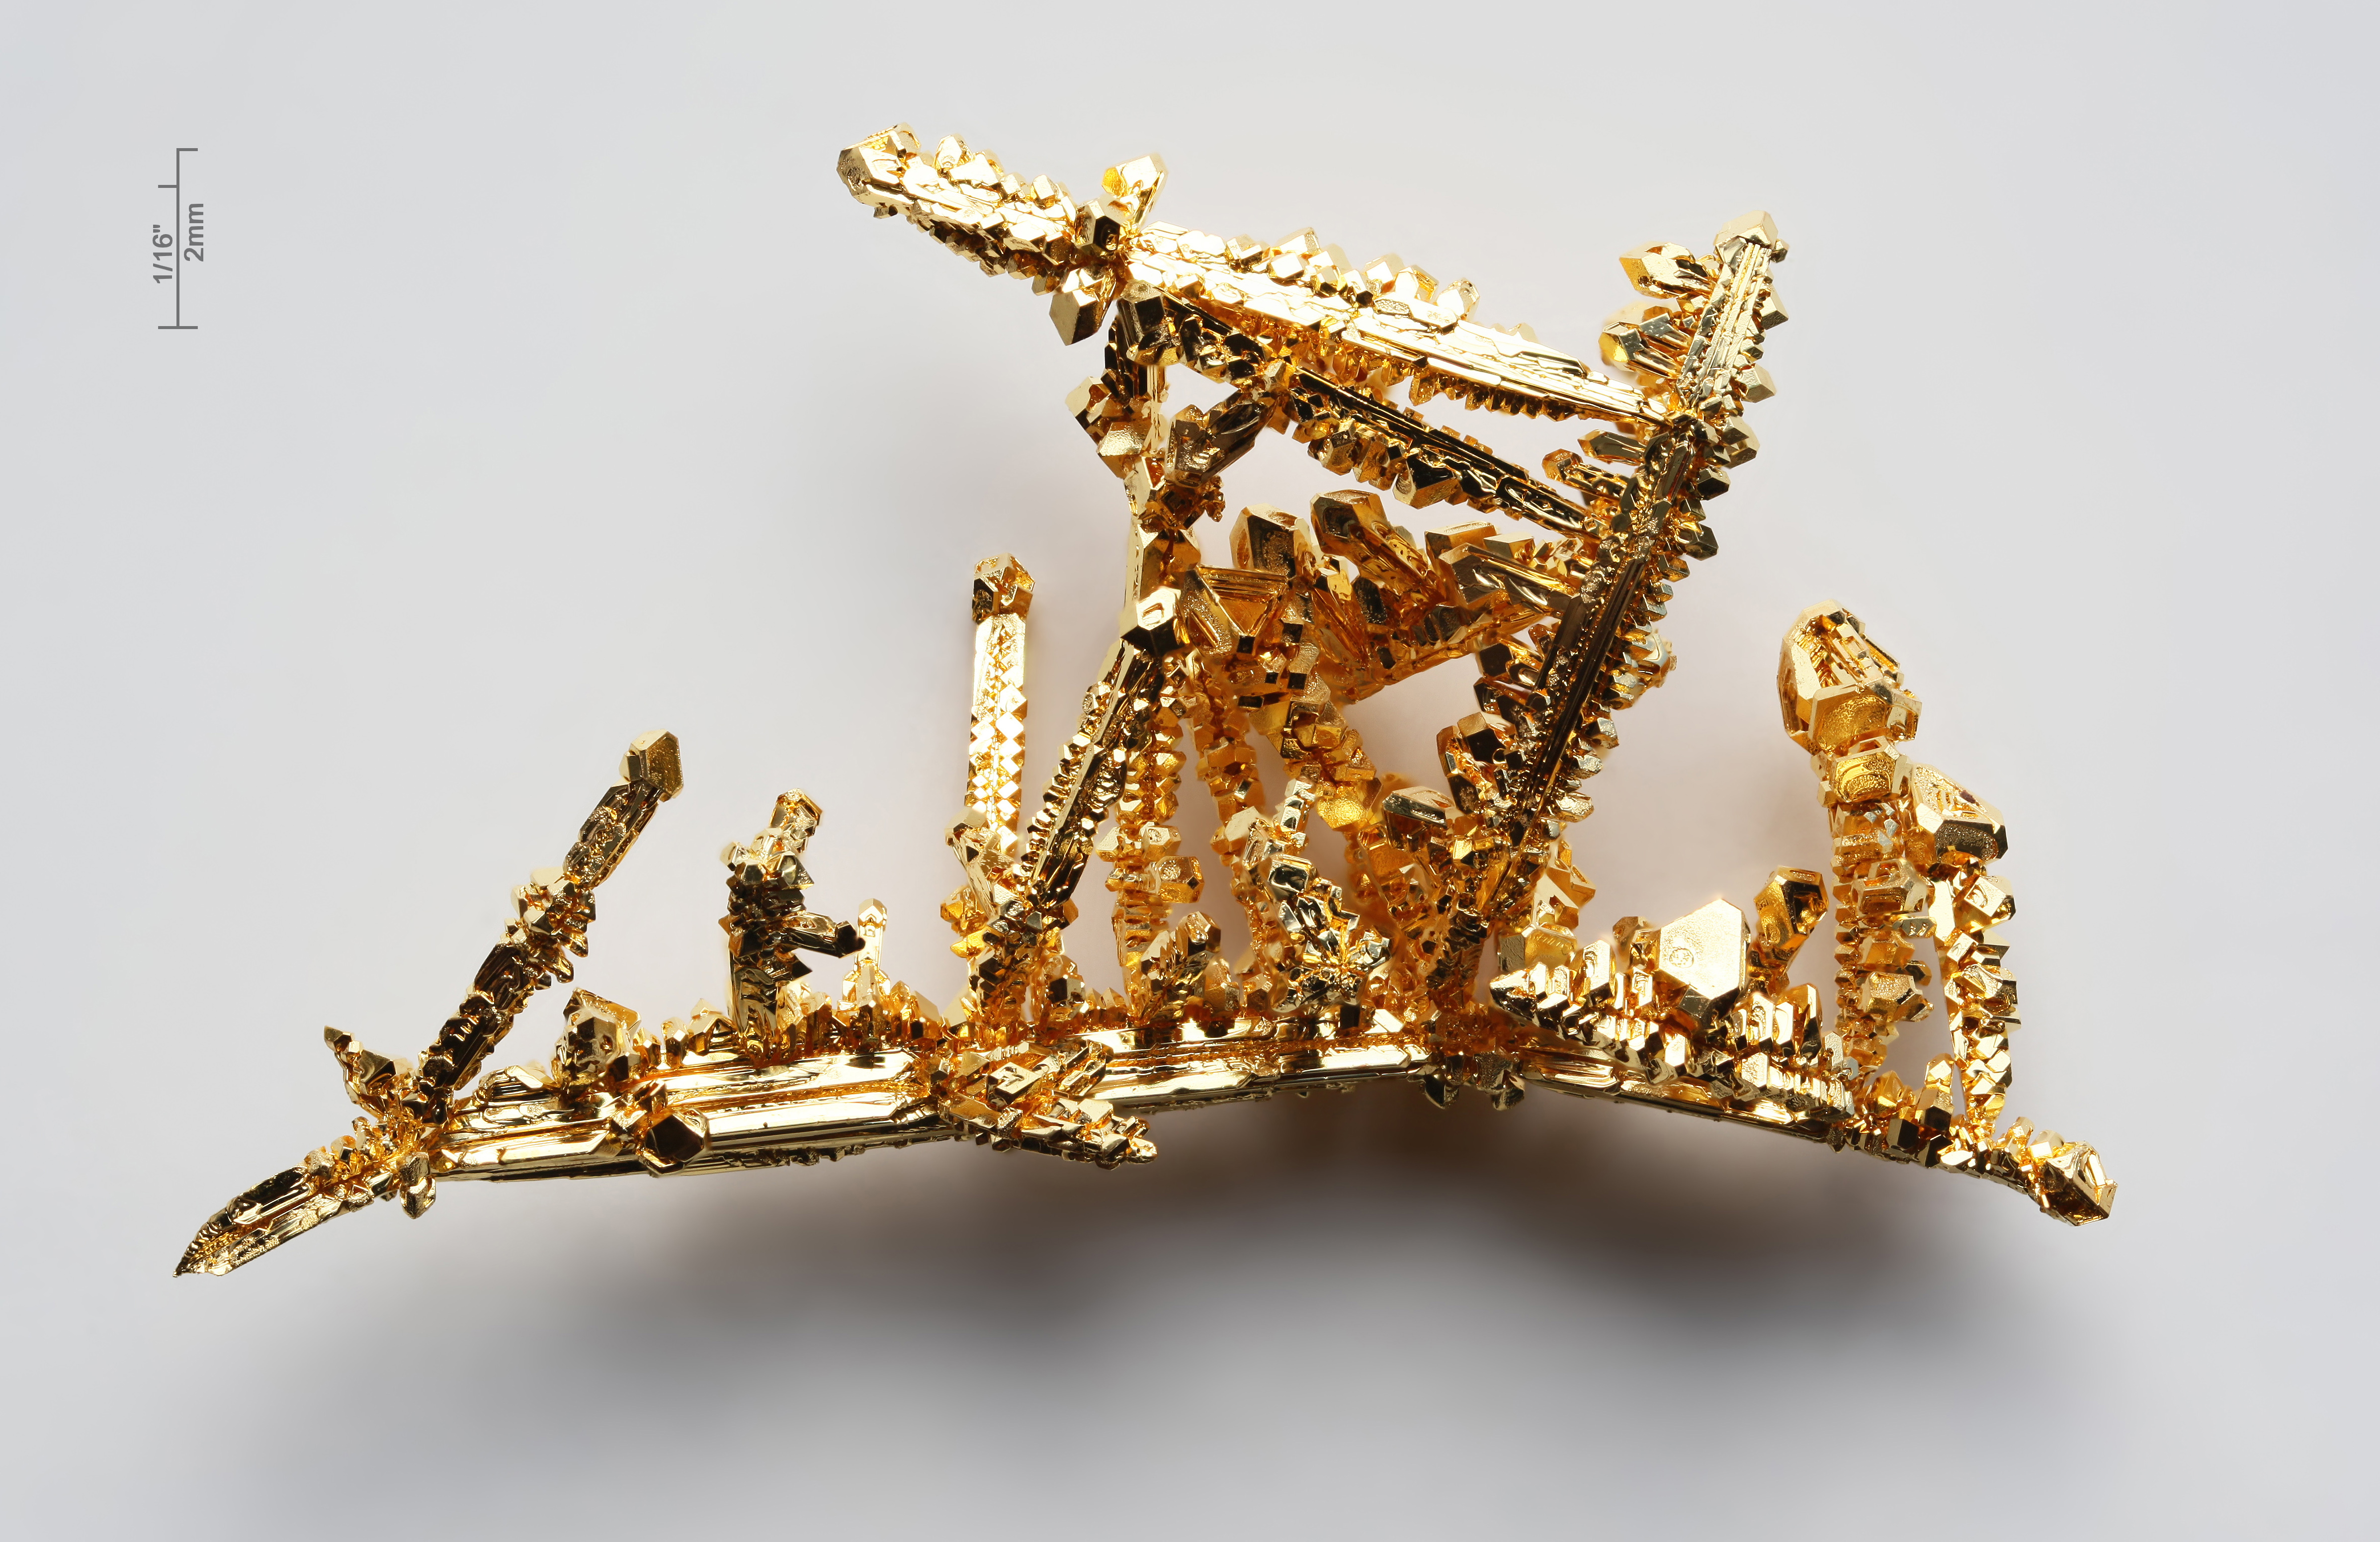
\includegraphics{chapter14/figure6}
%      \caption{ice, \ce{H2O(s)} is a molecular solid made of water molecules, whereas magnesium oxide \ce{MgO} is an ionic solid made of \ce{Mg^{2+}} cations and \ce{O^{2-}} anions. Gold is an atomic solid made of gold atoms.}
%   \end{marginfigure}
   


\begin{example} %%%%%%%%%%%%%%%%%%%%%%%% EXAMPLE BOX
Classify the following solids as ionic, molecular or atomic: diamond, dry ice (\ce{CO2}), iron and \ce{CaF2}.
\begin{center}
\begin{tabularx}{\textwidth}{
    >{\centering}m{.185\linewidth} 
    *{4}{Y} }
  \toprule
 & diamond   &\ce{CO2} &\ce{Fe}&\ce{CaF2}   \\
    \midrule
   Molecular  &     &  & & 	  		   \\
  Ionic&     &  & & 	 	     \\
      Atomic &     &  & & 		   		\\    
    \bottomrule
\end{tabularx}
\end{center}
\textlcsc{ \textcolor{dgreen}{\Large \textbf{Solution}} }\\
In general ionic solids correspond to ionic compounds and molecular solids correspond to covalent compounds. Therefore, dry ice should be a molecular solid and \ce{CaF2} and ionic solid. Iron and diamond are both made of atoms and hence they are atomic compounds.
\begin{tabularx}{\textwidth}{
    >{\centering}m{.185\linewidth} 
    *{4}{Y} }
  \toprule
 & diamond   &\ce{CO2} &\ce{Fe}&\ce{CaF2}   \\
    \midrule
   Molecular  &\xmark       &\checkmark	   &\xmark  &\xmark   	  		   \\
  Ionic&\xmark       &\xmark 	   &\xmark  &\checkmark  	 	     \\
      Atomic &\checkmark     &\xmark 	   &\xmark &\xmark  		   		\\    
            Metallic &\xmark      &\xmark 	   &\checkmark &\xmark  		   		\\    

    \bottomrule
\end{tabularx}
\\
\faDiamond\ \textlcsc{ \textcolor{dgreen}{\Large \textbf{Study Check}} }\\
Classify the following solids as ionic, molecular or atomic: silver, graphite, \ce{CaCO3} and \ce{NH3(s)}.
\begin{flushright} Answer: metallic, atomic, ionic and molecular.\end{flushright}
\end{example}%%%%%%%%%%%%%%%%%%%%%%%% EXAMPLE BOX

\end{description}
\newpage


\section{Metals and ionic solids}
Among the different types of crystalline solids, metals and ionic solids are very important. This section will cover the structure of metallic solids like gold or iron and ionic solids like sodium chloride.
\stepcounter{figurenewcounter}   \refstepcounter{figure}  \label{Fig:{\chapterlabel}\thefigurenewcounter}

\hspace{-5.5cm}\begin{minipage}[b]{1.5\linewidth}
\begin{center}\resizebox{1.0\textwidth}{!}{
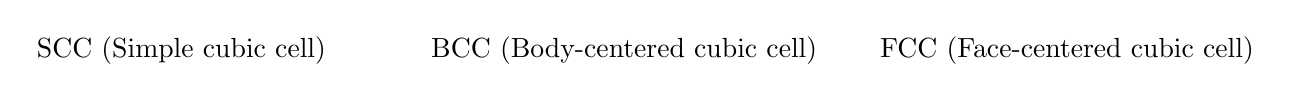
\begin{tikzpicture}[scale = 0.8]
\begin{scope}[shift={(-30em,0)}]
\SCUnitCell
\node [shift={(2em,-5em)}] {SCC (Simple cubic cell)};
\end{scope}
\begin{scope}[shift={(-10em,0)}]
\BccUnitCell
\node [shift={(2em,-5em)}] {BCC (Body-centered cubic cell)};
\end{scope}
\begin{scope}[shift={(10em,0)}]
\FccUnitCell
\node [shift={(2em,-5em)}] {FCC (Face-centered cubic cell)};
\end{scope}
\begin{scope}[shift={(-10em,-20em)},scale=1.0, every node/.append style={transform shape}]

\end{scope}
\end{tikzpicture}}\end{center}

\scalebox{0.4}{
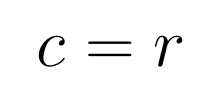
\begin{tikzpicture}
\sccSphere
\node[shift={(0,-5)}] {\Huge $c=r$};
 \end{tikzpicture}}\hspace{2.5cm}
\scalebox{0.4}{
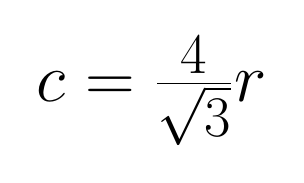
\begin{tikzpicture}
\bccSphere 
\node[shift={(0,-5)}] {\Huge $c=\frac{4}{\sqrt{3}}r$};
 \end{tikzpicture}}\hspace{2.0cm}
\scalebox{0.4}{
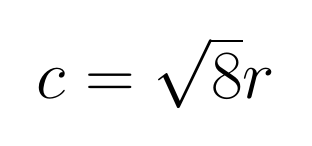
\begin{tikzpicture}
\fccSphere
\node[shift={(0,-5)}] {\Huge $c=\sqrt{8}r$};

 \end{tikzpicture}}
 \begin{tikzpicture}
 \node[text width=17cm, fontscale=.7] at (-30em,-30em) { \begin{bf}\color{black}\bfseries\large Figure \ref{Fig:{\chapterlabel}\thefigurenewcounter} \end{bf} The different unit cells. Space-fill structures are shown on the bottom. The simple cubic unit cells have atoms in the corners of the cell. The body-centered cubic unit cell have atoms in the corners and one atom in the center. The face-centered unit cell has atoms in the corners and in the faces. The relationship between the cell parameter ($c$) and the atomic radius ($r$) is also given for each unit cell. };
\end{tikzpicture}
\end{minipage}
\sloppy 
\begin{description}
   


\item[\docfilehook{Closed packing of metals}{}] 
Metallic solids result from the packing of metal atoms in space. Picture a single layer of spheres all packed together.  The most compact way to pack a layer of spheres is the situation in which one sphere is surrounded by six other spheres (layer A). This is called the closest packing. In this situation, every three spheres are connected by means of an indentation or dimple. Now let us think about how to pack a second layer on top of the first later. 
We can simply place the second layer just on top of the first layer (called layer A also). This would lead to a simple cubic packing arrangement (AA packing) which is not the most compact packing arrangement and the unit cell resulting from this packing is called \emph{simple cubic}. Differently, we could pack the second layer on the indentations of the first layer, which would lead to more complex packing schemes as we try to add a third layer. There would be two possible ways to add a third layer of atoms. You can locate the third layer on top of the first layer leading to an \ce{ABA} packing, with a resulting unit cell called \emph{hexagonal close cell, (hcp)}. Or you can locate the third layer on top of the indentations of the second layer leading to a \ce{ABC} layer packing leading to a unit cell called \emph{face centered cubic, (fcc)}. 


%\vspace{-1cm}
%\stepcounter{figurenewcounter}   \refstepcounter{figure}  \label{Fig:{\chapterlabel}\thefigurenewcounter}
%\begin{center}\resizebox{0.8\textwidth}{!}{
%\begin{tikzpicture}
%\def\rada{0.7}%
%\def\radb{1.4}%
%\def\shifta{6}%
%\def\shiftb{12}%
%\pgfmathsetmacro{\Cos}{\radb*cos(60)}%
%\pgfmathsetmacro{\Sin}{\radb*sin(60)}%
%\pgfmathsetmacro{\Sinc}{\radb*sin(60)/3}%
%
%\begin{scope}[xshift=0cm, yshift=0 cm]
%\shade[ball color=red,path fading=fade inside] (0,0) circle (\rada);
%\shade[ball color=red,path fading=fade inside] (\Cos cm,\Sin cm) circle (\rada);
%\shade[ball color=red,path fading=fade inside] (-\Cos cm,\Sin cm) circle (\rada);
%\shade[ball color=red,path fading=fade inside] (\Cos cm,-\Sin cm) circle (\rada);
%\shade[ball color=red,path fading=fade inside] (-\Cos cm,-\Sin cm) circle (\rada);
%\shade[ball color=red,path fading=fade inside] (-\radb cm,0 cm) circle (\rada);
%\shade[ball color=red,path fading=fade inside] (\radb cm,0 cm) circle (\rada);
%\end{scope}
%\begin{scope}[xshift=-\Cos cm, yshift= -\Sinc cm]
%\draw [blue, thick] (0,0) circle (\rada);
%\draw  [blue, thick] (\Cos cm,\Sin cm) circle (\rada);
%\draw  [blue, thick]  (-\Cos cm,\Sin cm) circle (\rada);
%\draw  [blue, thick] (\Cos cm,-\Sin cm) circle (\rada);
%\draw  [blue, thick] (-\Cos cm,-\Sin cm) circle (\rada);
%\draw [blue, thick]  (-\radb cm,0 cm) circle (\rada);
%\draw [blue, thick]  (\radb cm,0 cm) circle (\rada);
%\end{scope}
%
%\begin{scope}[xshift=\shifta cm, yshift=0 cm]
%\begin{scope}[xshift=0 cm, yshift=0 cm]
%\shade[ball color=red,path fading=fade inside] (0,0) circle (\rada);
%\shade[ball color=red,path fading=fade inside] (\Cos cm,\Sin cm) circle (\rada);
%\shade[ball color=red,path fading=fade inside] (-\Cos cm,\Sin cm) circle (\rada);
%\shade[ball color=red,path fading=fade inside] (\Cos cm,-\Sin cm) circle (\rada);
%\shade[ball color=red,path fading=fade inside] (-\Cos cm,-\Sin cm) circle (\rada);
%\shade[ball color=red,path fading=fade inside] (-\radb cm,0 cm) circle (\rada);
%\shade[ball color=red,path fading=fade inside] (\radb cm,0 cm) circle (\rada);
%\end{scope}
%\begin{scope}[xshift=-\Cos cm, yshift= -\Sinc cm]
%\shade[ball color=blue,path fading=fade inside] (0,0) circle (\rada);
%\shade[ball color=blue,path fading=fade inside] (\Cos cm,\Sin cm) circle (\rada);
%\shade[ball color=blue,path fading=fade inside]  (-\Cos cm,\Sin cm) circle (\rada);
%\shade[ball color=blue,path fading=fade inside] (\Cos cm,-\Sin cm) circle (\rada);
%\shade[ball color=blue,path fading=fade inside] (-\Cos cm,-\Sin cm) circle (\rada);
%\shade[ball color=blue,path fading=fade inside]  (-\radb cm,0 cm) circle (\rada);
%\shade[ball color=blue,path fading=fade inside]  (\radb cm,0 cm) circle (\rada);
%\end{scope}
%\begin{scope}[xshift=0 cm, yshift= 0 cm]
%\draw [red, thick] (0,0) circle (\rada);
%\draw [red, thick] (\Cos cm,\Sin cm) circle (\rada);
%\draw [red, thick]  (-\Cos cm,\Sin cm) circle (\rada);
%\draw [red, thick] (\Cos cm,-\Sin cm) circle (\rada);
%\draw [red, thick] (-\Cos cm,-\Sin cm) circle (\rada);
%\draw [red, thick]  (-\radb cm,0 cm) circle (\rada);
%\draw [red, thick]  (\radb cm,0 cm) circle (\rada);
%\end{scope}
%\end{scope}
%
%
%\def\shiftc{1.0}%
%\begin{scope}[xshift=\shiftb cm, yshift=-0.3 cm]
%\begin{scope}[xshift=-0.8*\shiftc cm, yshift=-0.8*\shiftc cm]
%\shade[ball color=red,path fading=fade inside] (0,\shiftc) circle (\rada);
%\shade[ball color=red,path fading=fade inside] (2*\rada,\shiftc) circle (\rada);
%\shade[ball color=red,path fading=fade inside] (-\shiftc*\rada,\shiftc*\rada) circle (\rada);
%\shade[ball color=red,path fading=fade inside] (-\shiftc*\rada+2*\rada,\shiftc*\rada) circle (\rada);
%\shade[ball color=red,path fading=fade inside] (-\shiftc*\rada+4*\rada,\shiftc*\rada) circle (\rada);
%\shade[ball color=red,path fading=fade inside] (0,0) circle (\rada);
%\shade[ball color=red,path fading=fade inside] (2*\rada,0) circle (\rada);
%\node[text width=3cm, xshift=-3em] at (-\shiftc*\rada+4*\rada-1.5 ,  \shiftc*\rada)  {\color{red} A};
%\end{scope}
%\begin{scope}[xshift=0 cm, yshift=0 cm]
%\shade[ball color=blue,path fading=fade inside] (0,\shiftc) circle (\rada);
%\shade[ball color=blue,path fading=fade inside] (2*\rada,\shiftc) circle (\rada);
%\shade[ball color=blue,path fading=fade inside] (-\shiftc*\rada,\shiftc*\rada) circle (\rada);
%\shade[ball color=blue,path fading=fade inside] (-\shiftc*\rada+2*\rada,\shiftc*\rada) circle (\rada);
%\shade[ball color=blue,path fading=fade inside] (-\shiftc*\rada+4*\rada,\shiftc*\rada) circle (\rada);
%\shade[ball color=blue,path fading=fade inside] (0,0) circle (\rada);
%\shade[ball color=blue,path fading=fade inside] (2*\rada,0) circle (\rada);
%\node[text width=3cm] at (-\shiftc*\rada+4*\rada+3.5 ,  \shiftc*\rada)  {\color{blue} B};
%\end{scope}
%\begin{scope}[xshift=-0.8*\shiftc cm, yshift=0.8*\shiftc cm]
%\shade[ball color=red,path fading=fade inside] (0,\shiftc) circle (\rada);
%\shade[ball color=red,path fading=fade inside] (2*\rada,\shiftc) circle (\rada);
%\shade[ball color=red,path fading=fade inside] (-\shiftc*\rada,\shiftc*\rada) circle (\rada);
%\shade[ball color=red,path fading=fade inside] (-\shiftc*\rada+2*\rada,\shiftc*\rada) circle (\rada);
%\shade[ball color=red,path fading=fade inside] (-\shiftc*\rada+4*\rada,\shiftc*\rada) circle (\rada);
%\shade[ball color=red,path fading=fade inside] (0,0) circle (\rada);
%\shade[ball color=red,path fading=fade inside] (2*\rada,0) circle (\rada);
%\node[text width=3cm, xshift=-3em] at (-\shiftc*\rada+4*\rada-1.5 ,  \shiftc*\rada)  {\color{red} A};
%\end{scope}
%\begin{scope}[xshift=0 cm, yshift=1.6*\shiftc cm]
%\shade[ball color=blue,path fading=fade inside] (0,\shiftc) circle (\rada);
%\shade[ball color=blue,path fading=fade inside] (2*\rada,\shiftc) circle (\rada);
%\shade[ball color=blue,path fading=fade inside] (-\shiftc*\rada,\shiftc*\rada) circle (\rada);
%\shade[ball color=blue,path fading=fade inside] (-\shiftc*\rada+2*\rada,\shiftc*\rada) circle (\rada);
%\shade[ball color=blue,path fading=fade inside] (-\shiftc*\rada+4*\rada,\shiftc*\rada) circle (\rada);
%\shade[ball color=blue,path fading=fade inside] (0,0) circle (\rada);
%\shade[ball color=blue,path fading=fade inside] (2*\rada,0) circle (\rada);
%\node[text width=3cm] at (-\shiftc*\rada+4*\rada+3.5 ,  \shiftc*\rada)  {\color{blue} B};
%\end{scope}
%\end{scope}
% \node[text width=9cm, fontscale=3.0] at (60em,-10em) { \begin{bf}\color{black}\bfseries\large Figure \ref{Fig:{\chapterlabel}\thefigurenewcounter} \end{bf} Different unit cells--such as sc, fcc or hcc--result from the different packing of metal layers. The simplest cubic structure results of placing two compact metal layer one on top of the other. When we place the second layer on the holes of the first layer we achieve a AB layer distribution and the resulting unit cell is called face centered unit cell. If we use a AB packing and now add a new layer on the holes of the second layer we obtain a ABC packing and the resulting unit cell is called hexagonal close cell. };
%
%\begin{scope}[xshift=0em, yshift=-20 em]
%
%
%\def\rada{0.7}%
%\def\radb{1.4}%
%\def\shifta{6}%
%\def\shiftb{12}%
%\pgfmathsetmacro{\Cos}{\radb*cos(60)}%
%\pgfmathsetmacro{\Sin}{\radb*sin(60)}%
%\pgfmathsetmacro{\Sinc}{\radb*sin(60)/3}%
%
%\begin{scope}[xshift=0cm, yshift=0 cm]
%\shade[ball color=red,path fading=fade inside] (0,0) circle (\rada);
%\shade[ball color=red,path fading=fade inside] (\Cos cm,\Sin cm) circle (\rada);
%\shade[ball color=red,path fading=fade inside] (-\Cos cm,\Sin cm) circle (\rada);
%\shade[ball color=red,path fading=fade inside] (\Cos cm,-\Sin cm) circle (\rada);
%\shade[ball color=red,path fading=fade inside] (-\Cos cm,-\Sin cm) circle (\rada);
%\shade[ball color=red,path fading=fade inside] (-\radb cm,0 cm) circle (\rada);
%\shade[ball color=red,path fading=fade inside] (\radb cm,0 cm) circle (\rada);
%\end{scope}
%\begin{scope}[xshift=-\Cos cm, yshift= -\Sinc cm]
%\draw [blue, thick] (0,0) circle (\rada);
%\draw  [blue, thick] (\Cos cm,\Sin cm) circle (\rada);
%\draw  [blue, thick]  (-\Cos cm,\Sin cm) circle (\rada);
%\draw  [blue, thick] (\Cos cm,-\Sin cm) circle (\rada);
%\draw  [blue, thick] (-\Cos cm,-\Sin cm) circle (\rada);
%\draw [blue, thick]  (-\radb cm,0 cm) circle (\rada);
%\draw [blue, thick]  (\radb cm,0 cm) circle (\rada);
%\end{scope}
%
%\begin{scope}[xshift=\shifta cm, yshift=0 cm]
%\begin{scope}[xshift=0 cm, yshift=0 cm]
%\shade[ball color=red,path fading=fade inside] (0,0) circle (\rada);
%\shade[ball color=red,path fading=fade inside] (\Cos cm,\Sin cm) circle (\rada);
%\shade[ball color=red,path fading=fade inside] (-\Cos cm,\Sin cm) circle (\rada);
%\shade[ball color=red,path fading=fade inside] (\Cos cm,-\Sin cm) circle (\rada);
%\shade[ball color=red,path fading=fade inside] (-\Cos cm,-\Sin cm) circle (\rada);
%\shade[ball color=red,path fading=fade inside] (-\radb cm,0 cm) circle (\rada);
%\shade[ball color=red,path fading=fade inside] (\radb cm,0 cm) circle (\rada);
%\end{scope}
%\begin{scope}[xshift=-\Cos cm, yshift= -\Sinc cm]
%\shade[ball color=blue,path fading=fade inside] (0,0) circle (\rada);
%\shade[ball color=blue,path fading=fade inside] (\Cos cm,\Sin cm) circle (\rada);
%\shade[ball color=blue,path fading=fade inside]  (-\Cos cm,\Sin cm) circle (\rada);
%\shade[ball color=blue,path fading=fade inside] (\Cos cm,-\Sin cm) circle (\rada);
%\shade[ball color=blue,path fading=fade inside] (-\Cos cm,-\Sin cm) circle (\rada);
%\shade[ball color=blue,path fading=fade inside]  (-\radb cm,0 cm) circle (\rada);
%\shade[ball color=blue,path fading=fade inside]  (\radb cm,0 cm) circle (\rada);
%\end{scope}
%\begin{scope}[xshift=0 cm, yshift= -1.5*\rada cm]
%\draw [green, thick] (0,0) circle (\rada);
%\draw [green, thick] (\Cos cm,\Sin cm) circle (\rada);
%\draw [green, thick]  (-\Cos cm,\Sin cm) circle (\rada);
%\draw [green, thick] (\Cos cm,-\Sin cm) circle (\rada);
%\draw [green, thick] (-\Cos cm,-\Sin cm) circle (\rada);
%\draw [green, thick]  (-\radb cm,0 cm) circle (\rada);
%\draw [green, thick]  (\radb cm,0 cm) circle (\rada);
%\end{scope}
%\end{scope}
%
%
%\def\shiftc{1.0}%
%\begin{scope}[xshift=\shiftb cm, yshift=-0.5 cm]
%
%\begin{scope}[xshift=-0.8*\shiftc cm, yshift=-0.8*\shiftc cm]
%\shade[ball color=red,path fading=fade inside] (0,\shiftc) circle (\rada);
%\shade[ball color=red,path fading=fade inside] (2*\rada,\shiftc) circle (\rada);
%\shade[ball color=red,path fading=fade inside] (-\shiftc*\rada,\shiftc*\rada) circle (\rada);
%\shade[ball color=red,path fading=fade inside] (-\shiftc*\rada+2*\rada,\shiftc*\rada) circle (\rada);
%\shade[ball color=red,path fading=fade inside] (-\shiftc*\rada+4*\rada,\shiftc*\rada) circle (\rada);
%\shade[ball color=red,path fading=fade inside] (0,0) circle (\rada);
%\shade[ball color=red,path fading=fade inside] (2*\rada,0) circle (\rada);
%\node[text width=3cm, xshift=-3em] at (-\shiftc*\rada+4*\rada-1.5 ,  \shiftc*\rada)  {\color{red} A};
%\end{scope}
%\begin{scope}[xshift=0 cm, yshift=0 cm]
%\shade[ball color=blue,path fading=fade inside] (0,\shiftc) circle (\rada);
%\shade[ball color=blue,path fading=fade inside] (2*\rada,\shiftc) circle (\rada);
%\shade[ball color=blue,path fading=fade inside] (-\shiftc*\rada,\shiftc*\rada) circle (\rada);
%\shade[ball color=blue,path fading=fade inside] (-\shiftc*\rada+2*\rada,\shiftc*\rada) circle (\rada);
%\shade[ball color=blue,path fading=fade inside] (-\shiftc*\rada+4*\rada,\shiftc*\rada) circle (\rada);
%\shade[ball color=blue,path fading=fade inside] (0,0) circle (\rada);
%\shade[ball color=blue,path fading=fade inside] (2*\rada,0) circle (\rada);
%\node[text width=3cm] at (-\shiftc*\rada+8*\rada,  -0.9*\shiftc*\rada)  {\color{blue} B};
%\end{scope}
%\begin{scope}[xshift=0.8*\shiftc cm, yshift=0.8*\shiftc cm]
%\shade[ball color=green,path fading=fade inside] (0,\shiftc) circle (\rada);
%\shade[ball color=green,path fading=fade inside] (2*\rada,\shiftc) circle (\rada);
%\shade[ball color=green,path fading=fade inside] (-\shiftc*\rada,\shiftc*\rada) circle (\rada);
%\shade[ball color=green,path fading=fade inside] (-\shiftc*\rada+2*\rada,\shiftc*\rada) circle (\rada);
%\shade[ball color=green,path fading=fade inside] (-\shiftc*\rada+4*\rada,\shiftc*\rada) circle (\rada);
%\shade[ball color=green,path fading=fade inside] (0,0) circle (\rada);
%\shade[ball color=green,path fading=fade inside] (2*\rada,0) circle (\rada);
%\node[text width=3cm] at (-\shiftc*\rada+9*\rada,\shiftc*\rada)  {\color{green} C};
%\end{scope}
%\begin{scope}[xshift=-0.8*\shiftc cm, yshift=1.6*\shiftc cm]
%\shade[ball color=red,path fading=fade inside] (0,\shiftc) circle (\rada);
%\shade[ball color=red,path fading=fade inside] (2*\rada,\shiftc) circle (\rada);
%\shade[ball color=red,path fading=fade inside] (-\shiftc*\rada,\shiftc*\rada) circle (\rada);
%\shade[ball color=red,path fading=fade inside] (-\shiftc*\rada+2*\rada,\shiftc*\rada) circle (\rada);
%\shade[ball color=red,path fading=fade inside] (-\shiftc*\rada+4*\rada,\shiftc*\rada) circle (\rada);
%\shade[ball color=red,path fading=fade inside] (0,0) circle (\rada);
%\shade[ball color=red,path fading=fade inside] (2*\rada,0) circle (\rada);
%\node[text width=3cm, xshift=-3em] at (-\shiftc*\rada+4*\rada-1.5 ,  \shiftc*\rada)  {\color{red} A};
%\end{scope}
%\end{scope}
%\end{scope}
%\end{tikzpicture}}\end{center}
%



%
%
%\begin{center}\resizebox{0.7\textwidth}{!}{
%\begin{tikzpicture}[scale=0.6]
%
%
%\end{tikzpicture}}\end{center}
%%\caption{}






%\begin{marginfigure}[-15cm]
%\begin{tcolorbox}[tab2,tabularx={>{\centering}m{.2\linewidth} *{1}{Y} }]%%%% FANCY COLOR TABLE
%
%%{>{\centering}m{.185\linewidth} *{1}{Y} }
%Structure & \begin{center}Atoms per  cell  \end{center}        \\\hline\hline
%sc&  1        \\\hline
%bcc &  2        \\\hline
%fcc &  4         
%\end{tcolorbox}%%%% FANCY COLOR TABLE
%\caption{Atoms per unit cell}
%\end{marginfigure}
%
%\begin{marginfigure}[-5cm]
%\begin{tcolorbox}[tab2,tabularx={>{\centering}m{.4\linewidth} *{1}{Y} }]%%%% FANCY COLOR TABLE
%
%%{>{\centering}m{.185\linewidth} *{1}{Y} }
%\begin{center}Location \end{center} & \begin{center}Sharing factor, $f$  \end{center}        \\\hline\hline
%Inside & 1        \\\hline
%Vertex&  $\nicefrac{1}{8}$        \\\hline
%Faces &  $\nicefrac{1}{2}$        \\\hline
%Edges &  $\nicefrac{1}{4}$         
%\end{tcolorbox}%%%% FANCY COLOR TABLE
%\caption{Sharing factors for different locations of a cubic unit cell}
%\end{marginfigure}








\item[\docfilehook{Atom sharing in unit cells}{}] Before we cover the different metallic units cells let us talk about atom sharing. Think about a cubit unit cell, that is a cube with one sphere (atom) in every corner of the cube. The whole lattice is produced by repeating the unit cell on the three dimensions. Hence, every corner of the cube is shared among other corders. This means, every corner--containing an atom--shares that atom with all units cells connected to that corner. Therefore, those atoms in the corner are not whole part of a single unit cell and they are shares. Every corner of a cube is shared among eight other cubes. Imagine pilling numerous boxes in layers. Every corner of each box is shared by three other boxes in the same plane and by four boxes on the plane on top--that is a total of eight boxes. They way you need to think of the different atoms in a single unit cell, is that they are shared depending on their location. As we discussed, corners of a cubic unit cell are shared by a total of 8 others unit cells. Atoms that belong to a face of a unit cell are shared by two unit cells. Atoms that are inside a unit cell fully belong to a single unit cell and they are not shared. Atoms that belong to a edge of the cube--an edge is the line that connects two vertexes of a cube--are shared by four units cells.



\begin{example} %%%%%%%%%%%%%%%%%%%%%%%% EXAMPLE BOX
The following structure is called face centered unit cell. This is a cubit unit cell with one atom in each corner of the cell and atoms also in the facets of the cell. Calculate the number of atoms in the unit cell:
\begin{center}
\begin{tikzpicture}[scale = 0.6]
%points on cube
\FccUnitCell
\end{tikzpicture}\end{center}

\textlcsc{ \textcolor{dgreen}{\Large \textbf{Solution}} }\\
If you count the number of spheres in the drawing you might think the cell contains fourteen atoms. However, this is not true, as each sphere is shared by other unit cells. Remember each location of the unit cell counts as a fraction. If an atom is fully inside in the cell--not in the vertexes, neither in the faces or sides--the sharing factor is one. If an atom belongs to a vertex, the sharing factor is $\nicefrac{1}{8}$. Atoms in a face has a sharing factor of $\nicefrac{1}{2}$ and atoms in the edges have a sharing factor of $\nicefrac{1}{4}$.
\begin{tabularx}{\textwidth}{
    >{\centering}m{.185\linewidth} 
    *{3}{Y} }
  \toprule
Location &Sharing Factor, $f$   &\# atoms, $N$	& $f\times N$		   \\
    \midrule
   Corner & 	$\nicefrac{1}{8}$ &8		& 1 		   \\
      Faces & 	$\nicefrac{1}{2}$&6		& 3 		   \\
    \bottomrule
\end{tabularx}
By multiplying the number of atoms in each location by the sharing factor and adding we obtain the total number of atoms in the cell. Overall, this unit cell has four atoms:
\\
\faDiamond\ \textlcsc{ \textcolor{dgreen}{\Large \textbf{Study Check}} }\\
The following structure is called simple body centered unit cell. This is a cubit unit cell with one atom in each corner of the cell and an atom also in the center of cell. Calculate the number of atoms in the unit cell:
\begin{center}
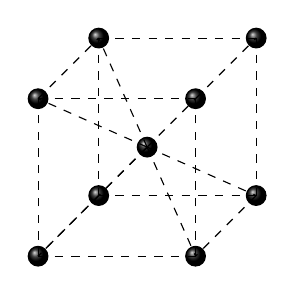
\begin{tikzpicture}[scale = 0.5]
%points on cube

\coordinate (A) at (0,0,0);
\coordinate (B) at (0,0,4);
\coordinate (D) at (0,4,0);
\coordinate (C) at (0,4,4);
\coordinate (E) at (4,0,0);
\coordinate (F) at (4,0,4);
\coordinate (H) at (4,4,0);
\coordinate (G) at (4,4,4);

%center of faces

\coordinate (I) at (0,2,2); %center of face ABCD
\coordinate (J) at (4,2,2); %center of face EFGH
\coordinate (K) at (2,4,2); %center of face DCGH
\coordinate (L) at (2,0,2); %center of face ABFE
\coordinate (M) at (2,2,4); %center of face CBGF
\coordinate (N) at (2,2,0); %center of face DAEH

%connectors

\coordinate (O) at (1,1,3);
\coordinate (P) at (1,3,1);
\coordinate (Q) at (3,1,1);
\coordinate (R) at (3,3,3);
%place non-atom cube corners
\shadedraw [ball color= black] (A) circle (0.25cm);
\shadedraw [ball color= black] (C) circle (0.25cm);
\shadedraw [ball color= black] (F) circle (0.25cm);
\shadedraw [ball color= black] (H) circle (0.25cm);
\shadedraw [ball color= black] (B) circle (0.25cm);
\shadedraw [ball color= black] (D) circle (0.25cm);
\shadedraw [ball color= black] (E) circle (0.25cm);
\shadedraw [ball color= black] (G) circle (0.25cm);
%draw the center of each face
\shadedraw [ball color= black] (2,2,2) circle (0.25cm);


%draw cube
\draw [dashed] (A) -- (B);
\draw [dashed] (B) -- (C);
\draw [dashed] (C) -- (D);
\draw [dashed] (D) -- (A);
\draw [dashed] (E) -- (F);
\draw [dashed] (F) -- (G);
\draw [dashed] (G) -- (H);
\draw [dashed] (H) -- (E);
\draw [dashed] (A) -- (E);
\draw [dashed] (B) -- (F);
\draw [dashed] (C) -- (G);
\draw [dashed] (D) -- (H);
\draw [dashed] (2,2,2) -- (A);\draw [dashed] (2,2,2) -- (B);\draw [dashed] (2,2,2) -- (C);\draw [dashed] (2,2,2) -- (D);\draw [dashed] (2,2,2) -- (E);\draw [dashed] (2,2,2) -- (F);\draw [dashed] (2,2,2) -- (G);
\end{tikzpicture}\end{center}
\begin{flushright} Answer: 2.\end{flushright}
\end{example}%%%%%%%%%%%%%%%%%%%%%%%% EXAMPLE BOX



\item[\docfilehook{Metal unit cells}{}] Here we will cover three different metal unit cells, all cubic cells. First, the simple cubic unit cell, with an atom each of the vertexes of the cell. This is the less compact unit cell with one atom per unit cell. Second, the body-centered unit cell is a cubic unit cell with atoms in the vertex of the cell and a single atom in the center of the cell. This cell has two atoms per unit cell. Third, the face-centered unit cell, with atoms in the vertex of the cell and also on the faces of the cell, on the sides of the cube. This is the most compact unit cell, with four atoms per cell. In the following image you can manipulate a face-centered cubic cell.

%\item[\docfilehook{An interactive fcc unit cell}{}] The fcc unit cell--remember fcc means face-centered cell--contain one atom in each corner of the cell and one atom also in each face of the unit cell. The next figure  is an interactive image. If you have installed the latest Acrobat reader version you will be able to manipulate the image and move it.
%
%
%\begin{figure}%%%%%%%%%%%%%%%%%%
%\begin{center}\vspace{2.5cm}
%
%\begin{asy}
%size(200);
%import solids;
%currentprojection=orthographic (
%camera=(8,5,4),
%up=(0,0,1),
%target=(2,2,2),
%zoom=0.5
%);
%
%// save predefined 2D orientation vectors
%pair NN=N;
%pair SS=S;
%pair EE=E;
%pair WW=W;
%
%//%points on cube
%
%triple A = (0,0,0);
%triple B = (0,0,4);
%triple D = (0,4,0);
%triple C = (0,4,4);
%triple E = (4,0,0);
%triple F = (4,0,4);
%triple H = (4,4,0);
%triple G = (4,4,4);
%
%triple[] cubicCornerA={  
%  A,C,F,H,
%};
%
%triple[] cubicCornerB={  
%  B,D,E,G,
%};
%
%
%//%center of faces
%
%triple I = (A+B+C+D)/4; //%center of face ABCD
%triple J = (E+F+G+H)/4; //%center of face EFGH
%triple K = (D+C+G+H)/4; //%center of face DCGH
%triple L = (A+B+F+E)/4; //%center of face ABFE
%triple M = (C+B+G+F)/4; //%center of face CBGF
%triple N = (D+A+E+H)/4; //%center of face DAEH
%
%triple[] faceCenter={  
%  I,J,K,L,M,N,
%};
%
%
%//%connectors
%triple O = (1,1,3);
%triple P = (1,3,1);
%triple Q = (3,1,1);
%triple R = (3,3,3);
%
%triple[] connectors={  
%  O,P,Q,R,
%};
%
%//%place non-atom cube corners
%
%real cornerAR=0.05;
%real cornerBR=0.6;
%real faceCR=0.2;
%real connR=faceCR;
%
%draw(A--B--C--D--cycle,darkblue+solid+linewidth(1));
%draw(E--F--G--H--cycle,darkblue+solid+linewidth(1));
%draw(A--E,darkblue+solid+linewidth(1));
%draw(B--F,darkblue+solid+linewidth(1));
%draw(C--G,darkblue+solid+linewidth(1));
%draw(D--H,darkblue+solid+linewidth(1));
%
%draw(A--I,dashed);
%draw(B--I,dashed);
%draw(C--I,dashed);
%draw(D--I,dashed);
%
%draw(E--J,dashed);
%draw(F--J,dashed);
%draw(G--J,dashed);
%draw(H--J,dashed);
%
%draw(D--K,dashed);
%draw(C--K,dashed);
%draw(G--K,dashed);
%draw(H--K,dashed);
%
%draw(A--L,dashed);
%draw(B--L,dashed);
%draw(F--L,dashed);
%draw(E--L,dashed);
%
%draw(C--M,dashed);
%draw(B--M,dashed);
%draw(G--M,dashed);
%draw(F--M,dashed);
%
%draw(D--N,dashed);
%draw(A--N,dashed);
%draw(E--N,dashed);
%draw(H--N,dashed);
%
%real cylR=0.062;
%
%void Draw(guide3 g,pen p=currentpen){
%  draw(
%    cylinder(
%      point(g,0),cylR,arclength(g),point(g,1)-point(g,0)
%    ).surface(
%               new pen(int i, real j){
%                 return p;
%               }
%             )
%  );
%}
%
%//%connections from faces to O
%//pen connectPen=lightgray;
%//Draw(B--O,connectPen);
%//Draw(I--O,connectPen);
%//Draw(M--O,connectPen);
%//Draw(L--O,connectPen);
%
%//%connections from faces to P
%//Draw(N--P,connectPen);
%//Draw(I--P,connectPen);
%//Draw(D--P,connectPen);
%//Draw(K--P,connectPen);
%
%//%connections from faces to Q
%//Draw(E--Q,connectPen);
%//Draw(J--Q,connectPen);
%//Draw(N--Q,connectPen);
%//Draw(L--Q,connectPen);
%
%//%connections from faces to R
%//Draw(G--R,connectPen);
%//Draw(M--R,connectPen);
%//Draw(J--R,connectPen);
%//Draw(K--R,connectPen);
%
%void drawSpheres(triple[] C, real R, pen p=currentpen){
%  for(int i=0;i<C.length;++i){
%    draw(sphere(C[i],R).surface(
%                        new pen(int i, real j){return p;}
%                        )
%    );
%  }
%}
%triple[] cubicCornerC={  
%  A,C,F,H,B,D,E,G,
%};
%
%//drawSpheres(cubicCornerA,cornerAR,darkgray);   //lightgray ; darkgray
%drawSpheres(cubicCornerC,cornerBR,lightblue);
%drawSpheres(faceCenter,cornerBR,lightblue);
%//drawSpheres(faceCenter,faceCR,red);
%//drawSpheres(connectors,connR,lightblue);
%\end{asy}
%\caption{A face-centered unit cell. This unit cell has one atom in each vertex of the cell and one atom in each face of the cell. Once we take into account the sharing factors of each position, this unit cell contains four atoms per unit cell and is the most compact of all cubit unit cells. \textbf{This image is interactive. With the latest Acrobat reader you will be able to manipulate it.}}
%   \setfloatalignment{t}
%
%\end{center}
%
%\end{figure}

%\begin{marginfigure}[5cm]
%\begin{tcolorbox}[tab2,tabularx={>{\centering}m{.4\linewidth} *{1}{Y} }]%%%% FANCY COLOR TABLE
%
%%{>{\centering}m{.185\linewidth} *{1}{Y} }
%Crystal structure & \begin{center}relation between $c$ and $r$  \end{center}        \\\hline\hline
%sc & $c=r$       \\\hline
%bcc&  $c=\nicefrac{4}{\sqrt{3}}r$        \\\hline
%fcc &  $c=\sqrt{8}r$	        \\\hline
%\end{tcolorbox}%%%% FANCY COLOR TABLE
%\caption{Relationship between cell parameter $c$ and atomic size $r$ for different types of unit cells}
%\end{marginfigure}
\item[\docfilehook{Cell parameter}{}] Cubic unit cells have the shape of a cube and hence all side of the cube have the same length. This length is called cell parameter $c$. Unit cells with large cell parameter have more spacing between atoms. The opposite is true for cells with smaller cell parameter. The cell parameter of a unit cell is related to the atomic radius. Let us analyze the case of a face-centered unit cell. In each side of the cell, in each face, we have four atoms in the vertexes and one in the center of the face. Of course these atoms do not belong only to this unit cell. However, if we symbolically cut the atoms in the face we can see the relation between the radius of the atom and the unit cell. The edges of the cell does not correspond to any cell parameter. However, the line that connect the bottom part with the opposite top part corresponds to a specific number of cell parameters, as the atoms are touching in this direction. In particular this distance is $4r$. Using Pythagoras theorem we have: $c^2+c^2=(4r)^2$. Therefore, $c=\sqrt{8}r$. 

 \savebox\trianglenew{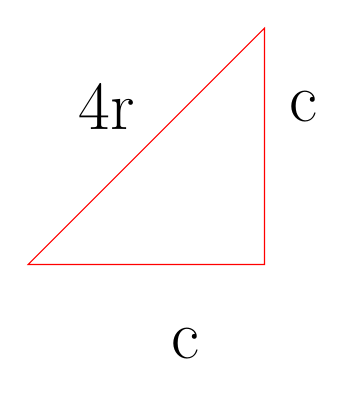
\begin{tikzpicture}\draw[red] (0,0) -- (3,0) -- (3,3) --cycle;\node[shift={(2,-1)}] {\Huge c}; \node[shift={(3.5,2.)}] {\Huge c}; \node[shift={(1,2)}] {\Huge 4r}; 
 \end{tikzpicture} }
%\stepcounter{figurenewcounter}   \refstepcounter{figure}  \label{Fig:{\chapterlabel}\thefigurenewcounter}
\begin{center}\scalebox{0.5}{
\begin{tikzpicture}

    \def\D{8} % cubic side length
%   \pgfmathsetmacro\R{\D/2} % sphere radius
    \pgfmathsetmacro\R{sqrt(2)/4*\D} % sphere radius
%   \pgfmathsetmacro\R{sqrt(3)/4*\D} % sphere radius
    \def\angEl{20} % elevation angle in interval [1,89]
    \def\angPh{10} % phase angle in interval [-44,44]
    \pgfmathsetmacro\uofx{cos(-135-\angPh)}
    \pgfmathsetmacro\vofx{sin(-135-\angPh)*sin(\angEl)}
    \pgfmathsetmacro\uofy{cos(-45-\angPh)}
    \pgfmathsetmacro\vofy{sin(-45-\angPh)*sin(\angEl)}
    \pgfmathsetmacro\uofz{0}
    \pgfmathsetmacro\vofz{cos(\angEl)}

    % The coordinates of the cube
    \begin{scope}[x={(\uofx cm,\vofx cm)}, y={(\uofy cm,\vofy cm)}, z={(\uofz cm,\vofz cm)}]
    \coordinate (C1) at (\D,0,0);
    \coordinate (C2) at (\D,0,\D);
    \coordinate (C3) at (0,0,\D);
    \coordinate (C4) at (0,\D,\D);
    \coordinate (C5) at (0,\D,0);
    \coordinate (C6) at (\D,\D,0);
    \coordinate (C7) at (0,0,0);
    \coordinate (C8) at (\D,\D,\D);
%    \foreach \n in {1,2,...,8} \node at (C\n) {C\n};

    \coordinate (C0) at ($(C2)!.5!(C5)$);
    \coordinate (S1) at ($(C2)!.5!(C6)$);
    \coordinate (S2) at ($(C2)!.5!(C4)$);
    \coordinate (S3) at ($(C8)!.5!(C5)$);
    \coordinate (S4) at ($(C6)!.5!(C7)$);
    \coordinate (S5) at ($(C1)!.5!(C3)$);
    \coordinate (S6) at ($(C5)!.5!(C3)$);
    \end{scope}

    % Draw the clipped spheres
    \ClippedEightSphere{+}{-}{+}{C7}
    \ClippedLongitudeSphere{S5}{45-\angPh}{+}
    \ClippedLongitudeSphere{S6}{135-\angPh}{-}
    \ClippedLatitudeSphere{S4}{0}{+}

    \ClippedEightSphere{-}{+}{-}{C8}
    \ClippedEightSphere{+}{-}{-}{C3}
    \ClippedEightSphere{+}{+}{-}{C2}
%   \fill[ball color=white] (C0) circle [radius=\R];
    \ClippedEightSphere{-}{-}{-}{C4}
    \ClippedEightSphere{+}{+}{+}{C1}
    \ClippedEightSphere{-}{-}{+}{C5}
    \ClippedEightSphere{-}{+}{+}{C6}

    % Draw the half spheres
    \ClippedLatitudeSphere{S2}{0}{-}
    \ClippedLongitudeSphere{S3}{45-\angPh}{-}
    \ClippedLongitudeSphere{S1}{135-\angPh}{+}
    \DrawLatitudeArc{S2}{0}{0}{360}
    \DrawLongitudeArc{S1}{135-\angPh}{0}{360}
    \DrawLongitudeArc{S3}{45-\angPh}{0}{360}

    % Draw the Arcs
    \DrawLongitudeArc{C1}{135-\angPh}{90}{90}
    \DrawLongitudeArc{C2}{135-\angPh}{-90}{-90}
    \DrawLongitudeArc{C4}{45-\angPh}{-90}{-90}
    \DrawLongitudeArc{C5}{45-\angPh}{90}{90}
    \DrawLongitudeArc{C6}{135-\angPh}{90}{-90}
    \DrawLongitudeArc{C6}{45-\angPh}{90}{-90}
    \DrawLongitudeArc{C8}{135-\angPh}{-90}{90}
    \DrawLongitudeArc{C8}{45-\angPh}{-90}{90}
    \DrawLatitudeArc{C2}{0}{45-\angPh}{-90}
    \DrawLatitudeArc{C3}{0}{-45-\angPh}{-90}
    \DrawLatitudeArc{C4}{0}{135-\angPh}{90}
    \DrawLatitudeArc{C8}{0}{135-\angPh}{-90}

    % Draw the cube
    \draw (C1)--(C2)--(C3)--(C4)--(C5)--(C6)--cycle;
    \draw (C2)--(C8)--(C6);
    \draw (C8)--(C4);

    % Radius node
    \coordinate (r) at ($(C2) - (\R/10,0)$);
    \LongitudePlane{\angEl}{135-\angPh}
    \draw [<->, current plane, line width=0.75mm, red] (C4) -- (C6) node [xshift=3cm, yshift=5.0cm] {\color{black} \Huge $4r$} ;
        \draw [<->, current plane, line width=0.75mm, red] (C6) -- (C5)  node [midway, xshift=1cm, yshift=-0.5cm] {\color{black}\Huge $c$};
        \draw [<->, current plane, line width=0.75mm, red] (C5) -- (C4)  node [midway, xshift=0.5cm, yshift=0cm] {\color{black}\Huge $c$};

%    \draw [<->, current plane] (r) -- node [left] {$r$} +(-90:\R);
 %\node[text width=16cm, fontscale=.7] at (-30em,-30em) { \begin{bf}\color{black}\bfseries\large Figure \ref{Fig:{\chapterlabel}\thefigurenewcounter} \end{bf} This is a space-filling representation of a fcc unit cell..};
%%%%%%%%%%%%%%%%%%%%%%%%%%%%
\coordinate (spy point) at (6em,3em);
\coordinate (magnifying glass) at (28em,6em);
\node [draw=none, shape=rectangle, inner sep=8.5em, postaction={decorate,decoration={raise=-0.6em, text along path,text align=right}}]  (a) at (magnifying glass) {};
\draw[draw=none, fill=gray, fill opacity=0.2] (spy point) to [bend left=-45] (a.south west) -- (a.north west)  to [bend right=-45]  (spy point) -- cycle;
\node  [thin, draw=black, shape=rectangle, inner sep=2.5em]  (c) at (magnifying glass) {\usebox\trianglenew} node[yshift=0.5em] at (c.north) {};
%%%%%%%%%%%%%%%%%%%%%%%%%%%%
  \node[shift={(9.5,-2)}] {\Huge $c^2+c^2=(4r)^2$};

\end{tikzpicture}
}\end{center}
%



\begin{example} %%%%%%%%%%%%%%%%%%%%%%%% EXAMPLE BOX
For the following unit cell, calculate the relationship between the cell parameter and the atomic radius. 
\begin{center}
\scalebox{0.2}{
\begin{tikzpicture}
%\newcommand\pgfmathsinandcos[3]{%
%  \pgfmathsetmacro#1{sin(#3)}%
%  \pgfmathsetmacro#2{cos(#3)}%
%}
%\newcommand\LongitudePlane[3][current plane]{%
%  \pgfmathsinandcos\sinEl\cosEl{#2} % elevation
%  \pgfmathsinandcos\sint\cost{#3} % azimuth
%  \tikzset{#1/.style={cm={\cost,\sint*\sinEl,0,\cosEl,(0,0)}}}
%}
%\newcommand\LatitudePlane[3][current plane]{%
%  \pgfmathsinandcos\sinEl\cosEl{#2} % elevation
%  \pgfmathsinandcos\sint\cost{#3} % latitude
%  \pgfmathsetmacro\yshift{\cosEl*\sint}
%  \tikzset{#1/.style={cm={\cost,0,0,\cost*\sinEl,(0,\yshift)}}}
%}
%
%%\newcommand\DrawLongitudeCircle[2][4]{
%%  \LongitudePlane{\angEl}{#2}
%%%  \tikzset{current plane/.prefix style={scale=#1}}
%%   % angle of "visibility"
%%  \pgfmathsetmacro\angVis{atan(sin(#2)*cos(\angEl)/sin(\angEl))}
%%  \draw[current plane, blue] (\angVis:\R) arc (\angVis:\angVis+180:\R);
%%  \draw[current plane, blue] (\angVis-180:\R) arc (\angVis-180:\angVis:\R);
%%}
%
%%\newcommand\DrawLatitudeCircle[2][5]{
%%  \LatitudePlane{\angEl}{#2}
%%%  \tikzset{current plane/.prefix style={scale=#1}}
%%%  \pgfmathsetmacro\sinVis{sin(#2)/cos(#2)*sin(\angEl)/cos(\angEl)}
%%%  % angle of "visibility"
%%%  \pgfmathsetmacro\angVis{asin(min(1,max(\sinVis,-1)))}
%%  \draw[current plane, red] (\angVis:\R) arc (\angVis:-\angVis-180:\R);
%%  \draw[current plane, red] (180-\angVis:\R) arc (180-\angVis:\angVis:\R);
%%}
%
%\newcommand\ClipLongitudeCircle[2]{
%    \LongitudePlane{\angEl}{#1}
%    \pgfmathsetmacro\angVis{atan(sin(#1)*cos(\angEl)/sin(\angEl))}
%    \path[save path=\tmppath, current plane] (\angVis:\R) arc (\angVis:\angVis+180:\R); % current plane transformation
%    \pgfoonew\patha=new spath(\tmppath)
%    \pgfmathsetmacro\angVis{-atan(sin(\angEl)*cos(#1)/sin(#1))}
%    \path[save path=\tmppath] (-90+\angVis:\R) arc (-90+\angVis:#2 180-90+\angVis:\R); % no coordinate transform (no current plane)
%    \pgfoonew\pathb=new spath(\tmppath)
%    \patha.concatenate with lineto(,\pathb)
%    \patha.close()
%    \patha.use path with tikz(clip)
%%   \patha.use path with tikz(fill=magenta, opacity=.2)
%%   \patha.use path with tikz(draw=magenta, very thick)
%}
%
%\newcommand\ClipLatitudeCircle[2]{
%    \LatitudePlane{\angEl}{#1}
%    \path[save path=\tmppath,current plane] (-180:\R) arc (-180:0:\R);
%    \pgfoonew\patha=new spath(\tmppath)
%    \path[save path=\tmppath] (0:\R) arc (0:#2 180:\R);
%    \pgfoonew\pathb=new spath(\tmppath)
%    \patha.concatenate with lineto(,\pathb)
%    \patha.close()
%    \patha.use path with tikz(clip)
%%   \patha.use path with tikz(fill=cyan, opacity=.2)
%%   \patha.use path with tikz(draw=cyan, very thick)
%}
%
%\newcommand\ClippedEightSphere[4]{
%\begin{scope}[transform canvas={shift=(#4)}]
%    \ClipLongitudeCircle{45-\angPh}{#1}
%    \ClipLongitudeCircle{135-\angPh}{#2}
%    \ClipLatitudeCircle{0}{#3}
%    \fill[ball color=white] (0,0) circle (\R);
%\end{scope}}
%
%\newcommand\ClippedLatitudeSphere[3]{
%\begin{scope}[transform canvas={shift=(#1)}]
%    \LatitudePlane{\angEl}{#2}
%    \ClipLatitudeCircle{0}{#3}
%    \fill[ball color=white] (0,0) circle [radius=\R];
%\end{scope}}
%
%\newcommand\ClippedLongitudeSphere[3]{
%\begin{scope}[transform canvas={shift=(#1)}]
%    \LongitudePlane{\angEl}{#2}
%    \ClipLongitudeCircle{#2}{#3}
%    \fill[ball color=white] (0,0) circle [radius=\R];
%\end{scope}}
%
%\newcommand\DrawLongitudeArc[4]{
%    \LongitudePlane{\angEl}{#2}
%    \begin{scope}[current plane, transform canvas={shift=(#1)}]
%    \fill [cyan] (0,0) -- ++(#3:\R) arc [start angle=#3, delta angle=#4, radius=\R] -- cycle;
%    \draw ++(#3:\R) arc [start angle=#3, delta angle=#4, radius=\R];
%    \end{scope}}
%
%\newcommand\DrawLatitudeArc[4]{
%    \LatitudePlane{\angEl}{#2}
%    \begin{scope}[current plane, transform canvas={shift=(#1)}]
%    \fill [cyan] (0,0) -- ++(#3:\R) arc [start angle=#3, delta angle=#4, radius=\R] -- cycle;
%    \draw ++(#3:\R) arc [start angle=#3, delta angle=#4, radius=\R];
%    \end{scope}}
%


    \def\D{8} % cubic side length
   \pgfmathsetmacro\R{\D/2} % sphere radius
%    \pgfmathsetmacro\R{sqrt(2)/4*\D} % sphere radius
%   \pgfmathsetmacro\R{sqrt(3)/4*\D} % sphere radius
    \def\angEl{20} % elevation angle in interval [1,89]
    \def\angPh{10} % phase angle in interval [-44,44]
    \pgfmathsetmacro\uofx{cos(-135-\angPh)}
    \pgfmathsetmacro\vofx{sin(-135-\angPh)*sin(\angEl)}
    \pgfmathsetmacro\uofy{cos(-45-\angPh)}
    \pgfmathsetmacro\vofy{sin(-45-\angPh)*sin(\angEl)}
    \pgfmathsetmacro\uofz{0}
    \pgfmathsetmacro\vofz{cos(\angEl)}

    % The coordinates of the cube
    \begin{scope}[x={(\uofx cm,\vofx cm)}, y={(\uofy cm,\vofy cm)}, z={(\uofz cm,\vofz cm)}]
    \coordinate (C1) at (\D,0,0);
    \coordinate (C2) at (\D,0,\D);
    \coordinate (C3) at (0,0,\D);
    \coordinate (C4) at (0,\D,\D);
    \coordinate (C5) at (0,\D,0);
    \coordinate (C6) at (\D,\D,0);
    \coordinate (C7) at (0,0,0);
    \coordinate (C8) at (\D,\D,\D);
%    \foreach \n in {1,2,...,8} \node at (C\n) {C\n};

    \coordinate (C0) at ($(C2)!.5!(C5)$);
    \coordinate (S1) at ($(C2)!.5!(C6)$);
    \coordinate (S2) at ($(C2)!.5!(C4)$);
    \coordinate (S3) at ($(C8)!.5!(C5)$);
    \coordinate (S4) at ($(C6)!.5!(C7)$);
    \coordinate (S5) at ($(C1)!.5!(C3)$);
    \coordinate (S6) at ($(C5)!.5!(C3)$);
    \end{scope}

    % Draw the clipped spheres
    \ClippedEightSphere{+}{-}{+}{C7}
    \ClippedLongitudeSphere{S5}{45-\angPh}{+}
    \ClippedLongitudeSphere{S6}{135-\angPh}{-}
    \ClippedLatitudeSphere{S4}{0}{+}

    \ClippedEightSphere{-}{+}{-}{C8}
    \ClippedEightSphere{+}{-}{-}{C3}
    \ClippedEightSphere{+}{+}{-}{C2}
 %  \fill[ball color=white] (C0) circle [radius=\R];
    \ClippedEightSphere{-}{-}{-}{C4}
    \ClippedEightSphere{+}{+}{+}{C1}
    \ClippedEightSphere{-}{-}{+}{C5}
    \ClippedEightSphere{-}{+}{+}{C6}

%    % Draw the half spheres
%    \ClippedLatitudeSphere{S2}{0}{-}
%    \ClippedLongitudeSphere{S3}{45-\angPh}{-}
%    \ClippedLongitudeSphere{S1}{135-\angPh}{+}
%    \DrawLatitudeArc{S2}{0}{0}{360}
%    \DrawLongitudeArc{S1}{135-\angPh}{0}{360}
%    \DrawLongitudeArc{S3}{45-\angPh}{0}{360}

    % Draw the Arcs
    \DrawLongitudeArc{C1}{135-\angPh}{90}{90}
    \DrawLongitudeArc{C2}{135-\angPh}{-90}{-90}
    \DrawLongitudeArc{C4}{45-\angPh}{-90}{-90}
    \DrawLongitudeArc{C5}{45-\angPh}{90}{90}
    \DrawLongitudeArc{C6}{135-\angPh}{90}{-90}
    \DrawLongitudeArc{C6}{45-\angPh}{90}{-90}
    \DrawLongitudeArc{C8}{135-\angPh}{-90}{90}
    \DrawLongitudeArc{C8}{45-\angPh}{-90}{90}
    \DrawLatitudeArc{C2}{0}{45-\angPh}{-90}
    \DrawLatitudeArc{C3}{0}{-45-\angPh}{-90}
    \DrawLatitudeArc{C4}{0}{135-\angPh}{90}
    \DrawLatitudeArc{C8}{0}{135-\angPh}{-90}

    % Draw the cube
    \draw (C1)--(C2)--(C3)--(C4)--(C5)--(C6)--cycle;
    \draw (C2)--(C8)--(C6);
    \draw (C8)--(C4);



\end{tikzpicture}
}
\end{center}

\textlcsc{ \textcolor{dgreen}{\Large \textbf{Solution}} }\\
For this unit cell, the atoms in the bottom part are touching. Hence, the cell parameter should be related to the atomic radius. In particular, two half atoms occupy the same distance as the cell parameter, so  $c=r$.
\\
\faDiamond\ \textlcsc{ \textcolor{dgreen}{\Large \textbf{Study Check}} }\\
For the following unit cell, calculate the relationship between the cell parameter and the atomic radius. 
\begin{center}
\scalebox{0.2}{
\begin{tikzpicture}
%\newcommand\pgfmathsinandcos[3]{%
%  \pgfmathsetmacro#1{sin(#3)}%
%  \pgfmathsetmacro#2{cos(#3)}%
%}
%\newcommand\LongitudePlane[3][current plane]{%
%  \pgfmathsinandcos\sinEl\cosEl{#2} % elevation
%  \pgfmathsinandcos\sint\cost{#3} % azimuth
%  \tikzset{#1/.style={cm={\cost,\sint*\sinEl,0,\cosEl,(0,0)}}}
%}
%\newcommand\LatitudePlane[3][current plane]{%
%  \pgfmathsinandcos\sinEl\cosEl{#2} % elevation
%  \pgfmathsinandcos\sint\cost{#3} % latitude
%  \pgfmathsetmacro\yshift{\cosEl*\sint}
%  \tikzset{#1/.style={cm={\cost,0,0,\cost*\sinEl,(0,\yshift)}}}
%}
%
%%\newcommand\DrawLongitudeCircle[2][4]{
%%  \LongitudePlane{\angEl}{#2}
%%%  \tikzset{current plane/.prefix style={scale=#1}}
%%   % angle of "visibility"
%%  \pgfmathsetmacro\angVis{atan(sin(#2)*cos(\angEl)/sin(\angEl))}
%%  \draw[current plane, blue] (\angVis:\R) arc (\angVis:\angVis+180:\R);
%%  \draw[current plane, blue] (\angVis-180:\R) arc (\angVis-180:\angVis:\R);
%%}
%
%%\newcommand\DrawLatitudeCircle[2][5]{
%%  \LatitudePlane{\angEl}{#2}
%%%  \tikzset{current plane/.prefix style={scale=#1}}
%%%  \pgfmathsetmacro\sinVis{sin(#2)/cos(#2)*sin(\angEl)/cos(\angEl)}
%%%  % angle of "visibility"
%%%  \pgfmathsetmacro\angVis{asin(min(1,max(\sinVis,-1)))}
%%  \draw[current plane, red] (\angVis:\R) arc (\angVis:-\angVis-180:\R);
%%  \draw[current plane, red] (180-\angVis:\R) arc (180-\angVis:\angVis:\R);
%%}
%
%\newcommand\ClipLongitudeCircle[2]{
%    \LongitudePlane{\angEl}{#1}
%    \pgfmathsetmacro\angVis{atan(sin(#1)*cos(\angEl)/sin(\angEl))}
%    \path[save path=\tmppath, current plane] (\angVis:\R) arc (\angVis:\angVis+180:\R); % current plane transformation
%    \pgfoonew\patha=new spath(\tmppath)
%    \pgfmathsetmacro\angVis{-atan(sin(\angEl)*cos(#1)/sin(#1))}
%    \path[save path=\tmppath] (-90+\angVis:\R) arc (-90+\angVis:#2 180-90+\angVis:\R); % no coordinate transform (no current plane)
%    \pgfoonew\pathb=new spath(\tmppath)
%    \patha.concatenate with lineto(,\pathb)
%    \patha.close()
%    \patha.use path with tikz(clip)
%%   \patha.use path with tikz(fill=magenta, opacity=.2)
%%   \patha.use path with tikz(draw=magenta, very thick)
%}
%
%\newcommand\ClipLatitudeCircle[2]{
%    \LatitudePlane{\angEl}{#1}
%    \path[save path=\tmppath,current plane] (-180:\R) arc (-180:0:\R);
%    \pgfoonew\patha=new spath(\tmppath)
%    \path[save path=\tmppath] (0:\R) arc (0:#2 180:\R);
%    \pgfoonew\pathb=new spath(\tmppath)
%    \patha.concatenate with lineto(,\pathb)
%    \patha.close()
%    \patha.use path with tikz(clip)
%%   \patha.use path with tikz(fill=cyan, opacity=.2)
%%   \patha.use path with tikz(draw=cyan, very thick)
%}
%
%\newcommand\ClippedEightSphere[4]{
%\begin{scope}[transform canvas={shift=(#4)}]
%    \ClipLongitudeCircle{45-\angPh}{#1}
%    \ClipLongitudeCircle{135-\angPh}{#2}
%    \ClipLatitudeCircle{0}{#3}
%    \fill[ball color=white] (0,0) circle (\R);
%\end{scope}}
%
%\newcommand\ClippedLatitudeSphere[3]{
%\begin{scope}[transform canvas={shift=(#1)}]
%    \LatitudePlane{\angEl}{#2}
%    \ClipLatitudeCircle{0}{#3}
%    \fill[ball color=white] (0,0) circle [radius=\R];
%\end{scope}}
%
%\newcommand\ClippedLongitudeSphere[3]{
%\begin{scope}[transform canvas={shift=(#1)}]
%    \LongitudePlane{\angEl}{#2}
%    \ClipLongitudeCircle{#2}{#3}
%    \fill[ball color=white] (0,0) circle [radius=\R];
%\end{scope}}
%
%\newcommand\DrawLongitudeArc[4]{
%    \LongitudePlane{\angEl}{#2}
%    \begin{scope}[current plane, transform canvas={shift=(#1)}]
%    \fill [cyan] (0,0) -- ++(#3:\R) arc [start angle=#3, delta angle=#4, radius=\R] -- cycle;
%    \draw ++(#3:\R) arc [start angle=#3, delta angle=#4, radius=\R];
%    \end{scope}}
%
%\newcommand\DrawLatitudeArc[4]{
%    \LatitudePlane{\angEl}{#2}
%    \begin{scope}[current plane, transform canvas={shift=(#1)}]
%    \fill [cyan] (0,0) -- ++(#3:\R) arc [start angle=#3, delta angle=#4, radius=\R] -- cycle;
%    \draw ++(#3:\R) arc [start angle=#3, delta angle=#4, radius=\R];
%    \end{scope}}
%


    \def\D{8} % cubic side length
 %  \pgfmathsetmacro\R{\D/2} % sphere radius
%    \pgfmathsetmacro\R{sqrt(2)/4*\D} % sphere radius
   \pgfmathsetmacro\R{sqrt(3)/4*\D} % sphere radius
    \def\angEl{20} % elevation angle in interval [1,89]
    \def\angPh{10} % phase angle in interval [-44,44]
    \pgfmathsetmacro\uofx{cos(-135-\angPh)}
    \pgfmathsetmacro\vofx{sin(-135-\angPh)*sin(\angEl)}
    \pgfmathsetmacro\uofy{cos(-45-\angPh)}
    \pgfmathsetmacro\vofy{sin(-45-\angPh)*sin(\angEl)}
    \pgfmathsetmacro\uofz{0}
    \pgfmathsetmacro\vofz{cos(\angEl)}

    % The coordinates of the cube
    \begin{scope}[x={(\uofx cm,\vofx cm)}, y={(\uofy cm,\vofy cm)}, z={(\uofz cm,\vofz cm)}]
    \coordinate (C1) at (\D,0,0);
    \coordinate (C2) at (\D,0,\D);
    \coordinate (C3) at (0,0,\D);
    \coordinate (C4) at (0,\D,\D);
    \coordinate (C5) at (0,\D,0);
    \coordinate (C6) at (\D,\D,0);
    \coordinate (C7) at (0,0,0);
    \coordinate (C8) at (\D,\D,\D);
%    \foreach \n in {1,2,...,8} \node at (C\n) {C\n};

    \coordinate (C0) at ($(C2)!.5!(C5)$);
    \coordinate (S1) at ($(C2)!.5!(C6)$);
    \coordinate (S2) at ($(C2)!.5!(C4)$);
    \coordinate (S3) at ($(C8)!.5!(C5)$);
    \coordinate (S4) at ($(C6)!.5!(C7)$);
    \coordinate (S5) at ($(C1)!.5!(C3)$);
    \coordinate (S6) at ($(C5)!.5!(C3)$);
    \end{scope}

    % Draw the clipped spheres
    \ClippedEightSphere{+}{-}{+}{C7}
    \ClippedLongitudeSphere{S5}{45-\angPh}{+}
    \ClippedLongitudeSphere{S6}{135-\angPh}{-}
    \ClippedLatitudeSphere{S4}{0}{+}

    \ClippedEightSphere{-}{+}{-}{C8}
    \ClippedEightSphere{+}{-}{-}{C3}
    \ClippedEightSphere{+}{+}{-}{C2}
   \fill[ball color=white] (C0) circle [radius=\R];
    \ClippedEightSphere{-}{-}{-}{C4}
    \ClippedEightSphere{+}{+}{+}{C1}
    \ClippedEightSphere{-}{-}{+}{C5}
    \ClippedEightSphere{-}{+}{+}{C6}

%    % Draw the half spheres
%    \ClippedLatitudeSphere{S2}{0}{-}
%    \ClippedLongitudeSphere{S3}{45-\angPh}{-}
%    \ClippedLongitudeSphere{S1}{135-\angPh}{+}
%    \DrawLatitudeArc{S2}{0}{0}{360}
%    \DrawLongitudeArc{S1}{135-\angPh}{0}{360}
%    \DrawLongitudeArc{S3}{45-\angPh}{0}{360}

    % Draw the Arcs
    \DrawLongitudeArc{C1}{135-\angPh}{90}{90}
    \DrawLongitudeArc{C2}{135-\angPh}{-90}{-90}
    \DrawLongitudeArc{C4}{45-\angPh}{-90}{-90}
    \DrawLongitudeArc{C5}{45-\angPh}{90}{90}
    \DrawLongitudeArc{C6}{135-\angPh}{90}{-90}
    \DrawLongitudeArc{C6}{45-\angPh}{90}{-90}
    \DrawLongitudeArc{C8}{135-\angPh}{-90}{90}
    \DrawLongitudeArc{C8}{45-\angPh}{-90}{90}
    \DrawLatitudeArc{C2}{0}{45-\angPh}{-90}
    \DrawLatitudeArc{C3}{0}{-45-\angPh}{-90}
    \DrawLatitudeArc{C4}{0}{135-\angPh}{90}
    \DrawLatitudeArc{C8}{0}{135-\angPh}{-90}

    % Draw the cube
    \draw (C1)--(C2)--(C3)--(C4)--(C5)--(C6)--cycle;
    \draw (C2)--(C8)--(C6);
    \draw (C8)--(C4);



\end{tikzpicture}
}
\end{center}

\begin{flushright} Answer: $c=\frac{4}{\sqrt{3}}r$.\end{flushright}
\end{example}%%%%%%%%%%%%%%%%%%%%%%%% EXAMPLE BOX


\item[\docfilehook{Metal density}{}] Different metals have different density. The value for density will depend on the cell parameter but also on the compacity of the unit cell, the more compact the unit cell the more atoms per cell and hence the more density. The formula that relates density with cell parameter and atoms per cell is:
%\resizeableyellownote{2.5}{1}{Add this formula to your flashcard.}
\begin{equation*}
\boxed{  d=\frac{N\cdot AW}{c^3\cdot 6.023\times 10^{-7}}  } \quad \textcolor{blue}{\text{Metallic density formula}}
\end{equation*}
where:
\begin{where}
 \item $d$   is the density in $g\cdot ml^{-1}$
 \item $N$   is the number of atoms per unit cell 
  \item $6.023\times 10^{-7}$ is related to the conversion between atoms and grams
 \item $AW$  is the atomic weight of the metal
  \item $c$  is the cell parameter in pm
\end{where}

\begin{example} %%%%%%%%%%%%%%%%%%%%%%%% EXAMPLE BOX
Calculate density of iron ($AW=55.845g\cdot mol^{-1}$) knowing this is a bcc metal with cell parameter is $286$pm. 
\\
\textlcsc{ \textcolor{dgreen}{\Large \textbf{Solution}} }\\
We know that iron is a bcc metal and hence it has two atoms per unit cell. Also we know its atomic weight $AW=55.845g\cdot mol^{-1}$ and the cell parameter $c=286$pm. Using the metallic density formula: 
\begin{equation*}
 d=\frac{2\cdot 55.845}{286^3\cdot 6.023\times 10^{-7}}=\frac{111.69 }{14.09}=7.93g\cdot ml^{-1}   
\end{equation*}
\\
\faDiamond\ \textlcsc{ \textcolor{dgreen}{\Large \textbf{Study Check}} }\\
Calculate density of gold (AW=$196.96g\cdot mol^{-1}$) knowing this is a fcc metal with cell parameter is $406$pm. 
\begin{flushright} Answer: $19.54g\cdot ml^{-1}$.\end{flushright}
\end{example}%%%%%%%%%%%%%%%%%%%%%%%% EXAMPLE BOX




\item[\docfilehook{Ionic solids}{}] Ionic solids have high melting point and they are typically hard. They also do not conduct the electricity in solid form. An example of an ionic solid is \ce{NaCl}. The structure of \ce{NaCl} and many other ionic solids results from the superposition of two different compact lattices--this is the reason these are called binary solids as they are made of two units--and each lattice is superimposed. Normally, the largest ion (\ce{Na^+}) forms a packed arrangement such as fcc or ccp, and the smallest ion (\ce{Cl^-}) resides on the holes of the lattice. Here we will care about constructing the formula of the unit cell, such as \ce{NaCl} by counting the atoms in the unit cell.


\begin{example} %%%%%%%%%%%%%%%%%%%%%%%% EXAMPLE BOX
Calculate the formula for the following unit cell
\begin{center}
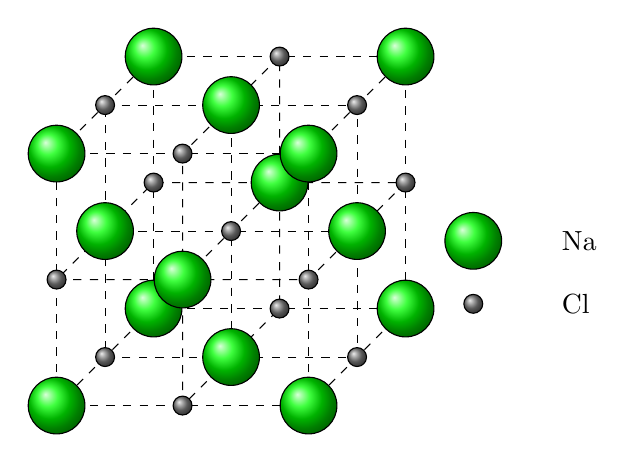
\begin{tikzpicture}[scale = 0.8]
%points on cube
\coordinate (A) at (0,0,0);
\coordinate (B) at (0,0,4);
\coordinate (D) at (0,4,0);
\coordinate (C) at (0,4,4);
\coordinate (E) at (4,0,0);
\coordinate (F) at (4,0,4);
\coordinate (H) at (4,4,0);
\coordinate (G) at (4,4,4);
%center of faces
\coordinate (I) at (0,2,2); %center of face ABCD
\coordinate (J) at (4,2,2); %center of face EFGH
\coordinate (K) at (2,4,2); %center of face DCGH
\coordinate (L) at (2,0,2); %center of face ABFE
\coordinate (M) at (2,2,4); %center of face CBGF
\coordinate (N) at (2,2,0); %center of face DAEH
%connectors
\coordinate (O) at (1,1,3);
\coordinate (P) at (1,3,1);
\coordinate (Q) at (3,1,1);
\coordinate (R) at (3,3,3);
%draw cube
\draw [dashed] (A) -- (B);
\draw [dashed] (B) -- (C);
\draw [dashed] (C) -- (D);
\draw [dashed] (D) -- (A);
\draw [dashed] (E) -- (F);
\draw [dashed] (F) -- (G);
\draw [dashed] (G) -- (H);
\draw [dashed] (H) -- (E);
\draw [dashed] (A) -- (E);
\draw [dashed] (B) -- (F);
\draw [dashed] (C) -- (G);
\draw [dashed] (D) -- (H);
%\draw [dashed] (2,2,2) -- (A);\draw [dashed] (2,2,2) -- (B);\draw [dashed] (2,2,2) -- (C);\draw [dashed] (2,2,2) -- (D);\draw [dashed] (2,2,2) -- (E);\draw [dashed] (2,2,2) -- (F);\draw [dashed] (2,2,2) -- (G);
\draw [dashed] (0,4,2) -- (4,4,2) -- (4,0,2)-- (0,0,2) -- cycle;
\draw [dashed] (2,4,0) -- (2,4,4) -- (2,0,4)-- (2,0,0) -- cycle;
\draw [dashed] (0,2,4)  -- (4,2,4) -- (4,2,0)  -- (0,2,0) -- cycle;
\draw [dashed] (I)  -- (J) ;
\draw [dashed] (K)  -- (L) ;
\draw [dashed] (M)  -- (N) ;
%Holes 
\coordinate (A1) at (0,4,2);
\coordinate (A2) at (4,4,2);
\coordinate (A3) at (4,0,2);
\coordinate (A4) at (0,0,2);
\coordinate (A5) at (2,4,0);
\coordinate (A6) at  (2,4,4);
\coordinate (A7) at (2,0,4);
\coordinate (A8) at (2,0,0);
\coordinate (A9) at (0,2,4);
\coordinate (A10) at (4,2,4);
\coordinate (A11) at (4,2,0);
\coordinate (A12) at (0,2,0);
\coordinate (A13) at (2,2,2);

%place non-atom cube corners
\shadedraw [ball color= green] (A) circle (0.45cm);
\shadedraw [ball color= green] (C) circle (0.45cm);
\shadedraw [ball color= green] (F) circle (0.45cm);
\shadedraw [ball color= green] (H) circle (0.45cm);
\shadedraw [ball color= green] (B) circle (0.45cm);
\shadedraw [ball color= green] (D) circle (0.45cm);
\shadedraw [ball color= green] (E) circle (0.45cm);
\shadedraw [ball color= green] (I) circle (0.45cm);
\shadedraw [ball color= green] (J) circle (0.45cm);
\shadedraw [ball color= green] (K) circle (0.45cm);
\shadedraw [ball color= green] (L) circle (0.45cm);
\shadedraw [ball color= green] (M) circle (0.45cm);
\shadedraw [ball color= green] (N) circle (0.45cm);
\shadedraw [ball color= green] (G) circle (0.45cm);


\shadedraw [ball color= gray] (A13) circle (0.15cm);
\shadedraw [ball color= gray] (A1) circle (0.15cm);
\shadedraw [ball color= gray] (A2) circle (0.15cm);
\shadedraw [ball color= gray] (A3) circle (0.15cm);
\shadedraw [ball color= gray] (A4) circle (0.15cm);
\shadedraw [ball color= gray] (A5) circle (0.15cm);
\shadedraw [ball color= gray] (A6) circle (0.15cm);
\shadedraw [ball color= gray] (A7) circle (0.15cm);
\shadedraw [ball color= gray] (A8) circle (0.15cm);
\shadedraw [ball color= gray] (A9) circle (0.15cm);
\shadedraw [ball color= gray] (A10) circle (0.15cm);
\shadedraw [ball color= gray] (A11) circle (0.15cm);
\shadedraw [ball color= gray] (A12) circle (0.15cm);

\shadedraw [ball color= gray, yshift=-2cm] (7,4,5) circle (0.15cm) node [right, xshift=1cm] {Cl};
\shadedraw [ball color= green, yshift=-2cm] (7,5,5) circle (0.45cm) node [right, xshift=1cm] {Na};

%draw the center of each face
\end{tikzpicture}\end{center}
\textlcsc{ \textcolor{dgreen}{\Large \textbf{Solution}} }\\
The unit cell contains \ce{Cl^-} and \ce{Na^+}. Remember every location in the unit cell has different sharing factor. We will compute the number of atoms in each location and multiply by the sharing factor to calculate the number of Cl and Na in the cell:
\begin{tabularx}{\textwidth}{
    >{\centering}m{.185\linewidth} 
    *{3}{Y} }
  \toprule
Location &Sharing Factor, $f$   &\# atoms, $N$	& $f\times N$		   \\
    \midrule
   Corner & 	$\nicefrac{1}{8}$ &8\ce{Na^+}		& 1 		   \\
      Faces & 	$\nicefrac{1}{2}$&6\ce{Na^+}		& 3 		   \\
            sides & 	$\nicefrac{1}{4}$&12\ce{Cl^-}		& 3 		   \\
            Inside & 	1&1\ce{Cl^-}		& 1 		   \\
    \bottomrule
\end{tabularx}
Overall, we have \ce{Na4Cl4} which corresponds with the formula \ce{NaCl}.\\
\faDiamond\ \textlcsc{ \textcolor{dgreen}{\Large \textbf{Study Check}} }\\
Calculate the formula for the following unit cell:
\begin{center}
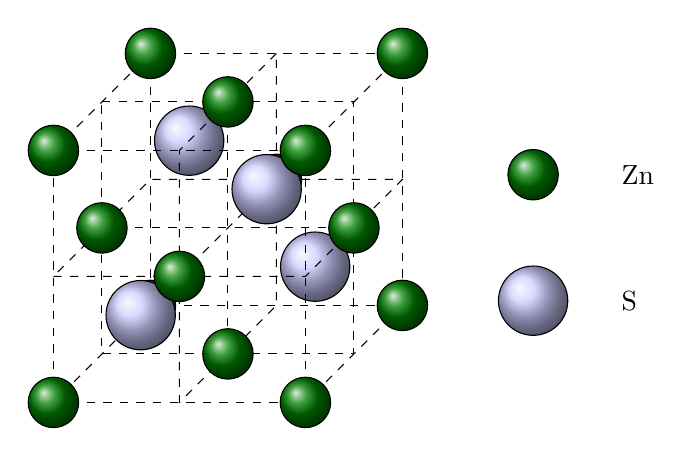
\begin{tikzpicture}[scale = 0.8]
%points on cube
\coordinate (A) at (0,0,0);
\coordinate (B) at (0,0,4);
\coordinate (D) at (0,4,0);
\coordinate (C) at (0,4,4);
\coordinate (E) at (4,0,0);
\coordinate (F) at (4,0,4);
\coordinate (H) at (4,4,0);
\coordinate (G) at (4,4,4);
%center of faces
\coordinate (I) at (0,2,2); %center of face ABCD
\coordinate (J) at (4,2,2); %center of face EFGH
\coordinate (K) at (2,4,2); %center of face DCGH
\coordinate (L) at (2,0,2); %center of face ABFE
\coordinate (M) at (2,2,4); %center of face CBGF
\coordinate (N) at (2,2,0); %center of face DAEH
%connectors
\coordinate (O) at (1,1,3);
\coordinate (P) at (1,3,1);
\coordinate (Q) at (3,1,1);
\coordinate (R) at (3,3,3);
\coordinate (B1) at (1,1,3);
\coordinate (B2) at (3,1,1);
\coordinate (B3) at (3,3,3);
\coordinate (B4) at (1,3,1);
\shadedraw [ball color= blue!20!white] (B2) circle (0.55cm);
\shadedraw [ball color= blue!20!white] (B4) circle (0.55cm);
%draw cube
\draw [dashed] (A) -- (B);
\draw [dashed] (B) -- (C);
\draw [dashed] (C) -- (D);
\draw [dashed] (D) -- (A);
\draw [dashed] (E) -- (F);
\draw [dashed] (F) -- (G);
\draw [dashed] (G) -- (H);
\draw [dashed] (H) -- (E);
\draw [dashed] (A) -- (E);
\draw [dashed] (B) -- (F);
\draw [dashed] (C) -- (G);
\draw [dashed] (D) -- (H);
%\draw [dashed] (2,2,2) -- (A);\draw [dashed] (2,2,2) -- (B);\draw [dashed] (2,2,2) -- (C);\draw [dashed] (2,2,2) -- (D);\draw [dashed] (2,2,2) -- (E);\draw [dashed] (2,2,2) -- (F);\draw [dashed] (2,2,2) -- (G);
\draw [dashed] (0,4,2) -- (4,4,2) -- (4,0,2)-- (0,0,2) -- cycle;
\draw [dashed] (2,4,0) -- (2,4,4) -- (2,0,4)-- (2,0,0) -- cycle;
\draw [dashed] (0,2,4)  -- (4,2,4) -- (4,2,0)  -- (0,2,0) -- cycle;
\draw [dashed] (I)  -- (J) ;
\draw [dashed] (K)  -- (L) ;
\draw [dashed] (M)  -- (N) ;
%Holes 
\coordinate (A1) at (0,4,2);
\coordinate (A2) at (4,4,2);
\coordinate (A3) at (4,0,2);
\coordinate (A4) at (0,0,2);
\coordinate (A5) at (2,4,0);
\coordinate (A6) at  (2,4,4);
\coordinate (A7) at (2,0,4);
\coordinate (A8) at (2,0,0);
\coordinate (A9) at (0,2,4);
\coordinate (A10) at (4,2,4);
\coordinate (A11) at (4,2,0);
\coordinate (A12) at (0,2,0);
\coordinate (A13) at (2,2,2);


%place non-atom cube corners

\shadedraw [ball color= green!50!black] (A) circle (0.40cm);
\shadedraw [ball color= green!50!black] (C) circle (0.40cm);
\shadedraw [ball color= green!50!black] (F) circle (0.40cm);
\shadedraw [ball color= green!50!black] (H) circle (0.40cm);
\shadedraw [ball color= green!50!black] (B) circle (0.40cm);
\shadedraw [ball color= green!50!black] (D) circle (0.40cm);
\shadedraw [ball color= green!50!black] (E) circle (0.40cm);
\shadedraw [ball color= green!50!black] (I) circle (0.40cm);
\shadedraw [ball color= green!50!black] (J) circle (0.40cm);
\shadedraw [ball color= green!50!black] (K) circle (0.40cm);
\shadedraw [ball color= green!50!black] (L) circle (0.40cm);
\shadedraw [ball color= green!50!black] (N) circle (0.40cm);
\shadedraw [ball color= blue!20!white] (B3) circle (0.55cm);

\shadedraw [ball color= blue!20!white] (B1) circle (0.55cm);


\shadedraw [ball color= green!50!black] (G) circle (0.40cm);


\shadedraw [ball color= green!50!black] (M) circle (0.40cm);


\shadedraw [ball color= blue!20!white, yshift=-2cm] (8,4,5) circle (0.55cm) node [right, xshift=1cm] {S};
\shadedraw [ball color= green!50!black, yshift=-2cm] (8,6,5) circle (0.40cm) node [right, xshift=1cm] {Zn};

%draw the center of each face
\end{tikzpicture}\end{center}

\begin{flushright} Answer: \ce{Zn4S4}.\end{flushright}
\end{example}%%%%%%%%%%%%%%%%%%%%%%%% EXAMPLE BOX

\item[\docfilehook{X-ray diffraction: a method to measure cell parameters}{}] 
X-ray diffraction is an experimental technique used to study the structure of solids and specifically to obtain cell parameters--the length of the unit cell that defines the structure of a crystal. X-rays, high-frequency radiation, scatter when they encounter a regular array of atoms in which the spacing is compatible with the x-ray wavelength. Diffraction results in two different types of wave interference: constrictive and destructive. Constructive interference results in bright spots and destructive interference results in dark spots. Waves impacting atoms at a different lattice positions travel different distances. If the difference in distance equals to an integral number of wavelength there both rays will interfere constructively.
\stepcounter{figurenewcounter}   \refstepcounter{figure}  \label{Fig:{\chapterlabel}\thefigurenewcounter}

 \begin{center}\resizebox{1\textwidth}{!}{\begin{tikzpicture}
    [x={(0.866cm,-0.5cm)}, y={(0.866cm,0.5cm)}, z={(0cm,1cm)}, scale=1.0,
%    [x={(1cm,0cm)}, y={(0.866cm,0.5cm)}, z={(0cm,1cm)}, scale=1.0,
    %Option for nice arrows
    >=stealth, %
    inner sep=0pt, outer sep=2pt,%
    axis/.style={thick,->},
    wave/.style={thick,color=#1,smooth},
    polaroid/.style={fill=black!60!white, opacity=0.3},]

    % Colors
    \colorlet{darkgreen}{green!50!black}
    \colorlet{lightgreen}{green!80!black}
    \colorlet{darkred}{red!50!black}
    \colorlet{lightred}{red!80!black}

    % Frame
 
%
%    \draw[thick,dashed] (-2,0,0) -- (O);
\draw (.5,.5) to [bend right=45]  (0,0.8) node[shift={(1em,-0.6em)}] {$\theta$};
\draw (-.7,-.7) to [bend right=-45]  (-1.2,-0.1) node[shift={(-0.9em,-0.9em)}] {$\theta$};
\draw[draw=none,fill=blue,fill opacity=0.2] (-30em,0) rectangle (31em,-15em);
\begin{scope}[rotate=65, shift={(0em,0em)}]
   \coordinate (O) at (0, 0, 0);
    \draw  (O) -- +(14, 0,   0) node [right] { };
%    \draw[axis] (O) -- +(0,  14, 0) node [right] {y};
    \draw (O) -- +(0,  0,   14) node [above] { };
\draw[wave=blue, variable=\x,samples at={0,0.25,...,10}]
    plot (\x,{sin(2*\x r)},0)node[anchor=north, shift={(0em,1em)}]{\huge Reflected x-ray};
    \draw[wave=blue, variable=\z,samples at={0,0.25,...,10}]
    plot (0,{sin(2*\z r)},\z)node[anchor=north,shift={(0em,1em)}]{\huge Incident x-ray};
    \draw[fill=black] (O) circle (1mm) node[shift={(-0em,2em)}] {A};
        \draw[fill=black] ([shift={(-3.7em,8em)}]O) circle (1mm) ;
        \draw[fill=black] ([shift={(-7.9em,17em)}]O) circle (1mm) ;
        \draw[fill=black] ([shift={(-12em,26em)}]O) circle (1mm) ;
     \draw[fill=black] ([shift={(3.7em,-8em)}]O) circle (1mm) ;
        \draw[fill=black] ([shift={(7.9em,-17em)}]O) circle (1mm) ;
        \draw[fill=black] ([shift={(12em,-26em)}]O) circle (1mm) ;
    \draw (O) -- +(12em,-26em) node [above] { };
    \draw (O) -- +(-12em,26em) node [above] { };


\end{scope}

\begin{scope}[rotate=65, shift={(-4em,-10.2em)}]
%   \coordinate (O) at (0, 0, 0);
%    \draw (O) -- +(0,  0,   14) node [above] { };
\draw[wave=green, variable=\x,samples at={0,0.25,...,10}] plot (\x,{sin(2*\x r)},0)node[anchor=north]{ };
\end{scope}

\begin{scope}[rotate=65, shift={(-12em,4em)}]
    \draw[wave=green, variable=\z,samples at={0,0.25,...,10}]
    plot (0,{sin(2*\z r)},\z)node[anchor=north]{ };
\end{scope}

\begin{scope}[rotate=65, shift={(-12em,-5.5em)}]
   \coordinate (O) at (0, 0, 0);
    \draw  (0em,0,0) -- +(20, 0,   0) node [right] { };
        \draw (O) -- +(0,  0,   14) node [above] { };

    \end{scope}
    \begin{scope}[rotate=0, shift={(-0em,-0em)}]
            \draw (O) -- +(0,  0,   4.6) --+(-1.75,  -1.75,   1.4)    node[shift={(-0em,-1em)}] {B};
            \draw (O) -- +(0,  0,   4.6) --+(1.52,  1.52,   1.85) node[shift={(-0em,-1em)}] {D} node[rotate=42,shift={(-4em,2em)}] {d sin $\theta$} node[rotate=-30,shift={(-8em,-7.8em)}] {d sin $\theta$};
              \draw[fill=black] ( O) circle (1mm) node[shift={(-0em,-1em)}] {C} node[shift={(1em,6em)}] {d};

  \draw[fill=black] ([shift={(9.2em,0em)}]O) circle (1mm) ;
  \draw[fill=black] ([shift={(18.4em,0em)}]O) circle (1mm) ;
  \draw[fill=black] ([shift={(27.6em,0em)}]O) circle (1mm) ;
  \draw[fill=black] ([shift={(-9.2em,0em)}]O) circle (1mm) ;
  \draw[fill=black] ([shift={(-18.4em,0em)}]O) circle (1mm) ;
  \draw[fill=black] ([shift={(-27.6em,0em)}]O) circle (1mm) ;
    \draw (O) -- +(27.6em,0em) node [above] { };
    \draw (O) -- +(-27.6em,0em) node [above] { };
        \end{scope}
%\draw [shift={(-0em,-1.5em)}](1,0) arc(15:-38:1) node[shift={(1em,-0.6em)}] {$\theta$};
%\draw [shift={(-5em,-1.5em)}](1,0) arc(-135:0:.4) node[shift={(-1.3em,-0.6em)}] {$\theta$};
%%%%%%%%%%%%%%%%%%%%%%%%%%%%
\coordinate (spy point) at (6em,3em);
\coordinate (magnifying glass) at (9em,17.5em);
\node [draw=none, shape=circle, inner sep=4.5em, postaction={decorate,decoration={raise=-0.6em, text along path,text align=right,text={|\tiny\color{black}|{\textsuperscript{\textcopyright}} Wikipedia}}}]  (a) at (magnifying glass) {};
\draw[draw=none, fill=gray, fill opacity=0.2] (spy point) to [bend left=45] (a.west) -- (a.east)  to [bend right=45]  (spy point) -- cycle;
\node  [thin, draw=black, shape=circle, inner sep=4.5em, fill overzoom image=chapter14/figure16]  (c) at (magnifying glass) {} node[yshift=0.5em] at (c.north) {\huge X-ray diffraction pattern};
%%%%%%%%%%%%%%%%%%%%%%%%%%%%
\end{tikzpicture}}\end{center}

\begin{tikzpicture}
\node[text width=12cm, fontscale=.3] at (-0em,-0em) { \begin{bf}\color{black}\bfseries\large Figure \ref{Fig:{\chapterlabel}\thefigurenewcounter} \end{bf} Reflection of x-rays in two different lattice points separated by a distance. The incident waves are in phase--maximums and minimums overlap-- but the reflected waves are only in face when the different of distances traveled by both is a integral number of wavelengths. In the image $BC+CD=2d sin\theta$.};

\end{tikzpicture}
Bragg's equation relate the cell parameter ($d$) of a solid with the angle ($\theta$) of the diffracted x-rays and its wavelength ($\lambda$). The number $n$ is called the diffraction order and represents an integer values ($n$=0, 1, 2, $\dots$).
\begin{equation}
n\lambda = 2d sin\theta
\end{equation}

\begin{example} %%%%%%%%%%%%%%%%%%%%%%%% EXAMPLE BOX
We study the structure of a crystal using x-rays of 9nm, finding a first-order reflection at 20$^{\circ}$. Calculate the distance between the planes responsible for this reflection.
\\
\textlcsc{ \textcolor{dgreen}{\Large \textbf{Solution}} }\\
We should use Bragg's equation, using $\theta$=20$^{\circ}$, $\lambda$=9nm and $n$=1. Solving for $d$ we have:
\[1\cdot 9 = 2d sin(20)\]
The calculated plane spacing is 26.3nm.
\\
\faDiamond\ \textlcsc{ \textcolor{dgreen}{\Large \textbf{Study Check}} }\\
Two lattice planes separated by a distance of 4nm produce a first-order x-ray diffraction at 15$^{\circ}$ using radiation of wavelength of 3.2nm. Calculate the angle for the second-order diffraction.
\begin{flushright} Answer: 53$^{\circ}$  \end{flushright}
\end{example}%%%%%%%%%%%%%%%%%%%%%%%% EXAMPLE BOX


\end{description}

\newpage
\section{Liquid state}
This section will cover some of the properties of the liquid state. In particular the importance of the vapor pressure, the viscosity and the surface tension. All these properties are determined by the intermolecular forces that connect the molecules of a liquid.
\sloppy 
\begin{description}
   \begin{marginfigure}[0cm]
   \begin{tikzpicture} \node (a) at (0,0) {\includegraphics[width=4cm, height=4cm]{chapter14/figure7}} node[rotate=90, font=\tiny] at ([yshift=.5cm,xshift=.1cm]a.south east) {\textsuperscript{\textcopyright} wikipedia} ;
\node[text width=5cm] at ([yshift=0.2cm]a.north) {\mytriangle{red}A paper clip standing on water};
\end{tikzpicture}
\begin{tikzpicture} \node (a) at (0,0) {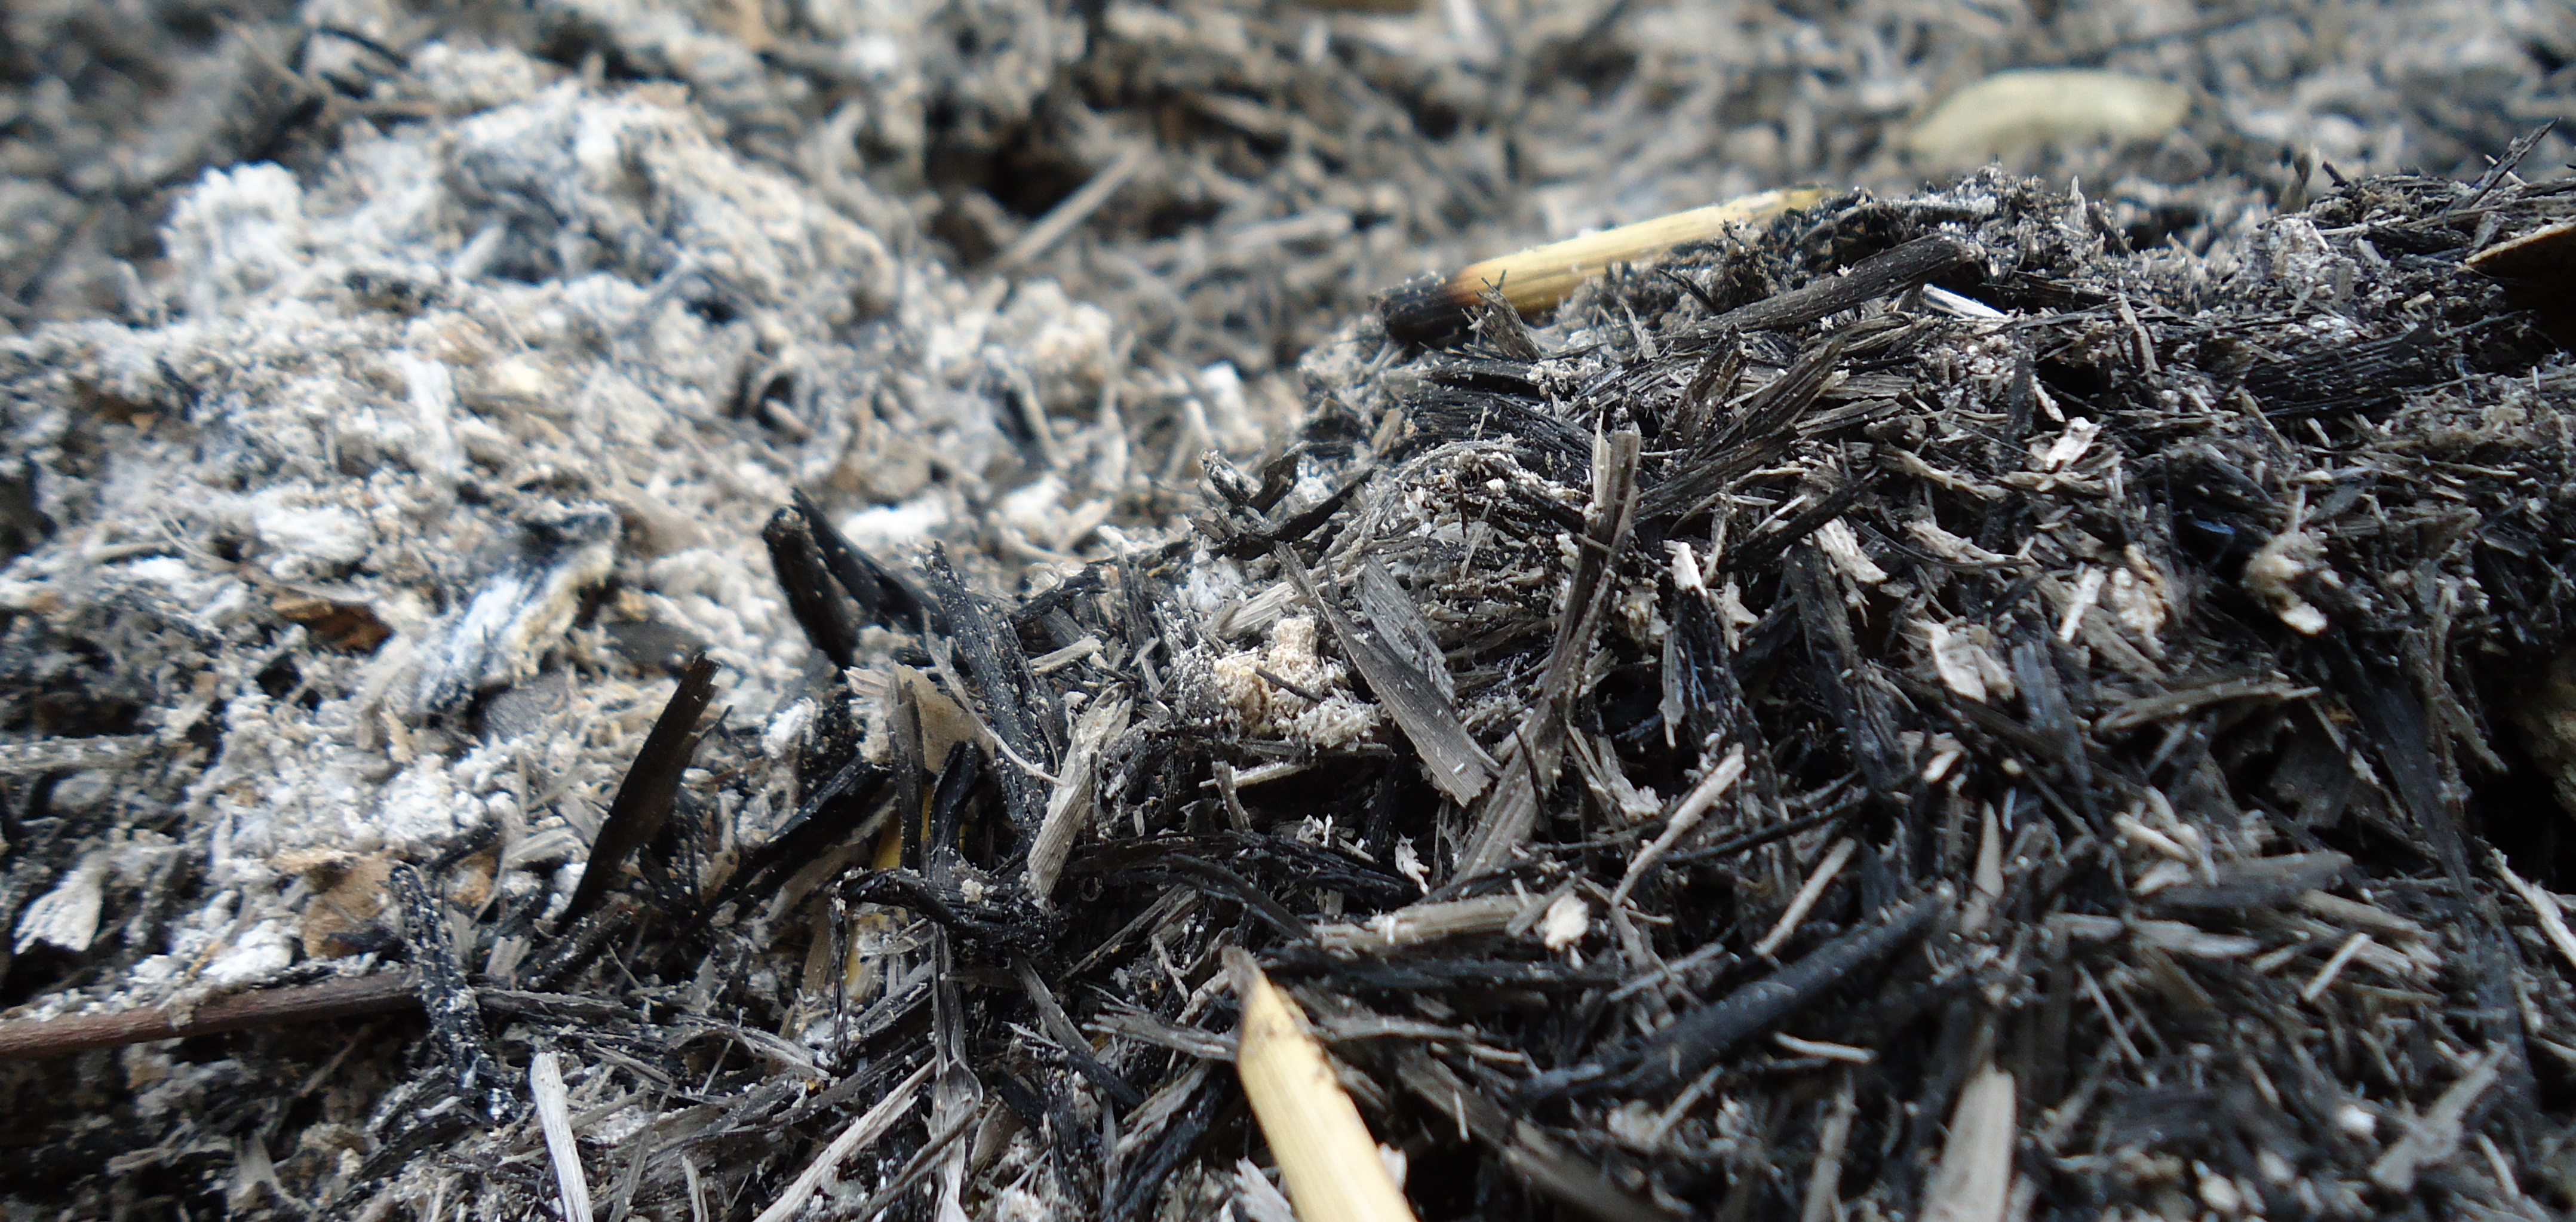
\includegraphics[width=4cm, height=4cm]{chapter14/figure8}} node[rotate=90, font=\tiny] at ([yshift=.5cm,xshift=.1cm]a.south east) {\textsuperscript{\textcopyright} www.pickist.com} ;
\node[text width=5cm] at ([yshift=0.2cm]a.north) {\mytriangle{red}Water droplets};
\end{tikzpicture}
\begin{tikzpicture} \node (a) at (0,0) {\includegraphics[width=4cm, height=4cm]{chapter14/figure9}} node[rotate=90, font=\tiny] at ([yshift=.5cm,xshift=.1cm]a.south east) {\textsuperscript{\textcopyright} Flickr} ;
\node[text width=5cm] at ([yshift=0.2cm]a.north) {\mytriangle{red}Meniscus of water and mercury};
\end{tikzpicture}
\begin{tikzpicture} \node (a) at (0,0) {\includegraphics[width=4cm, height=4cm]{chapter14/figure10}} node[rotate=90, font=\tiny] at ([yshift=.5cm,xshift=.1cm]a.south east) {\textsuperscript{\textcopyright} Flickr} ;
\node[text width=5cm] at ([yshift=0.2cm]a.north) {\mytriangle{red}A viscous liquid};
\end{tikzpicture}
\begin{tikzpicture} \node (a) at (0,0) {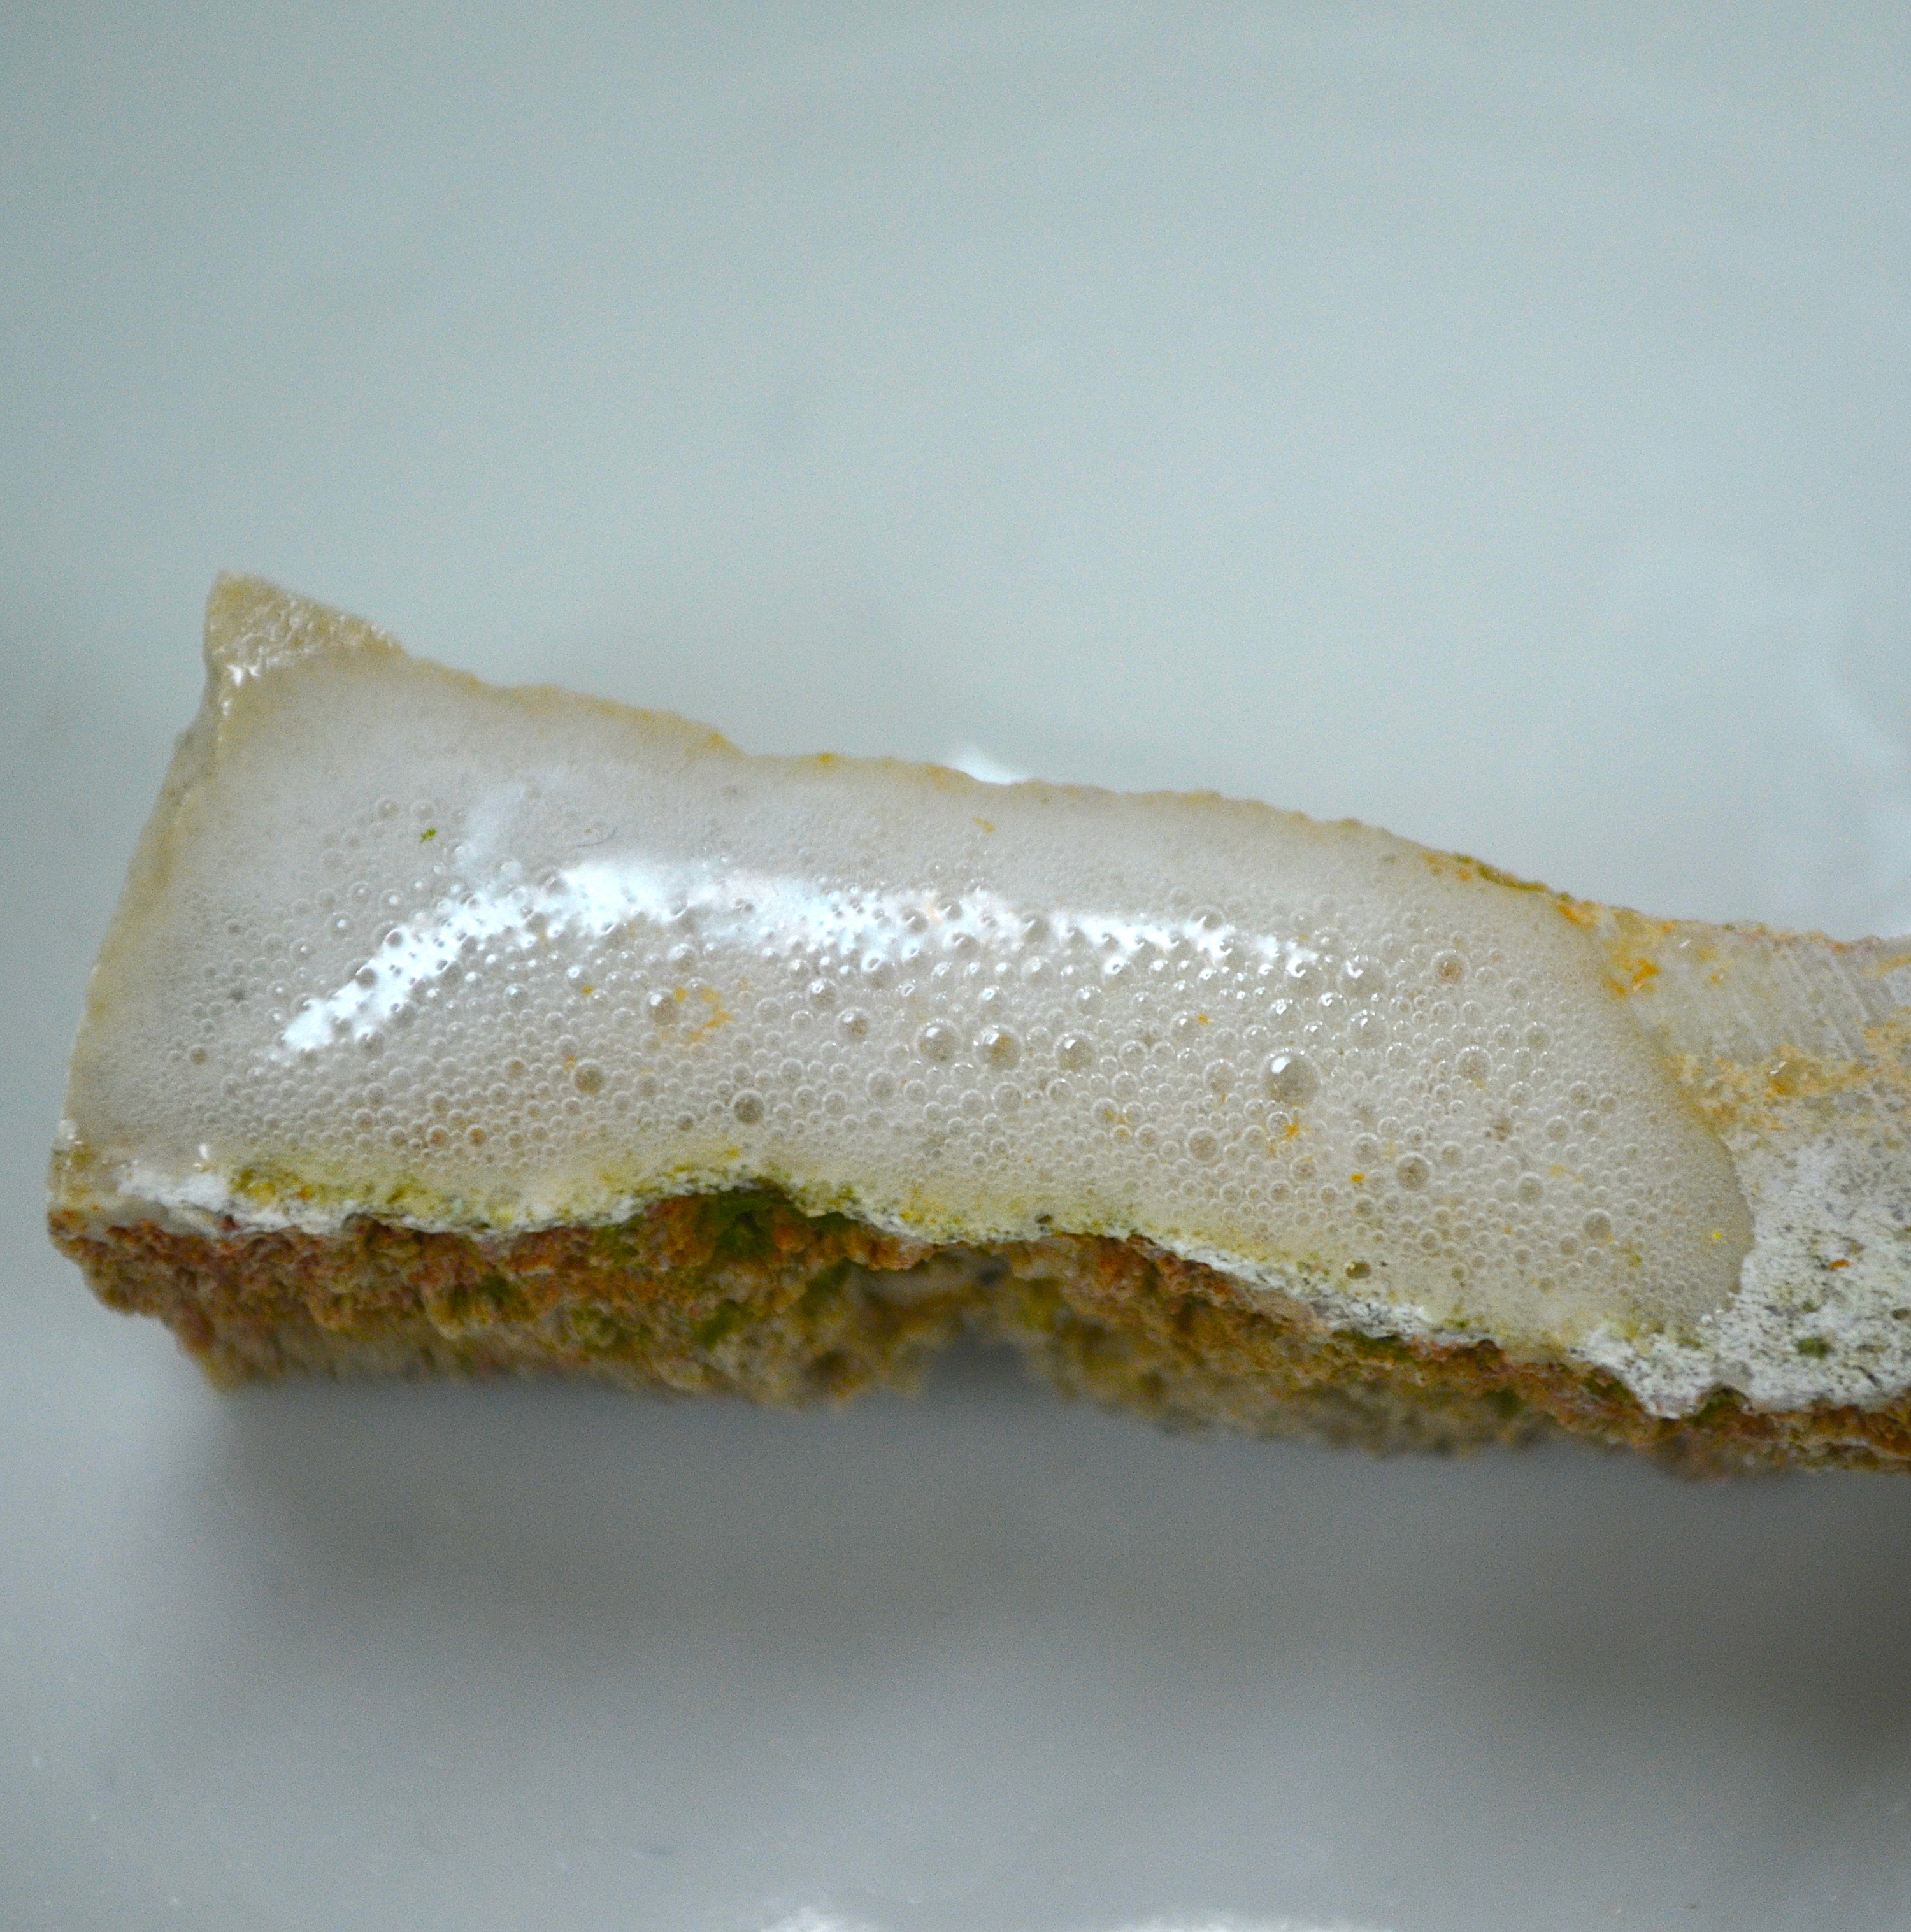
\includegraphics[width=4cm, height=6cm ]{chapter14/figure11}} node[rotate=90, font=\tiny] at ([yshift=.5cm,xshift=.1cm]a.south east) {\textsuperscript{\textcopyright} wikipedia} ;
\node[text width=5cm] at ([yshift=0.2cm]a.north) {\mytriangle{red}Capillary for tubes of different diameters};
\end{tikzpicture}
%\caption{Some properties of liquids}
%\label{fig:marginfig2}
\end{marginfigure}



\item[\docfilehook{Surface tension}{}] In a liquid the are two types of molecules, based on their location. Some molecules are located in the interior part of the liquid, far away from its surface. We call this the bulk of the liquid. Others are located at the surface of the liquid. The molecules at the bulk are pulled in all directions by the intermolecular forces so that overall there is no net pull in any direction. The molecules at the surface are pulled down and to the side by the surrounding molecules. However, they are not pulled up and hence they experience a new pull inward that causes the surface of the liquid to tighten up so that the surface minimizes its surface area. The surface tension of a liquid ($\gamma_t$) is a measure of the elastic force in the surface of the liquid. It is defined as the amount of energy needed to modify the surface of a liquid by unit of area, with units of milli Newton per meter, mN/m.
\vspace{-0cm}
\stepcounter{figurenewcounter}   \refstepcounter{figure}  \label{Fig:{\chapterlabel}\thefigurenewcounter}
     \begin{center}
     
     
 \resizebox{0.4\textwidth}{!}{%
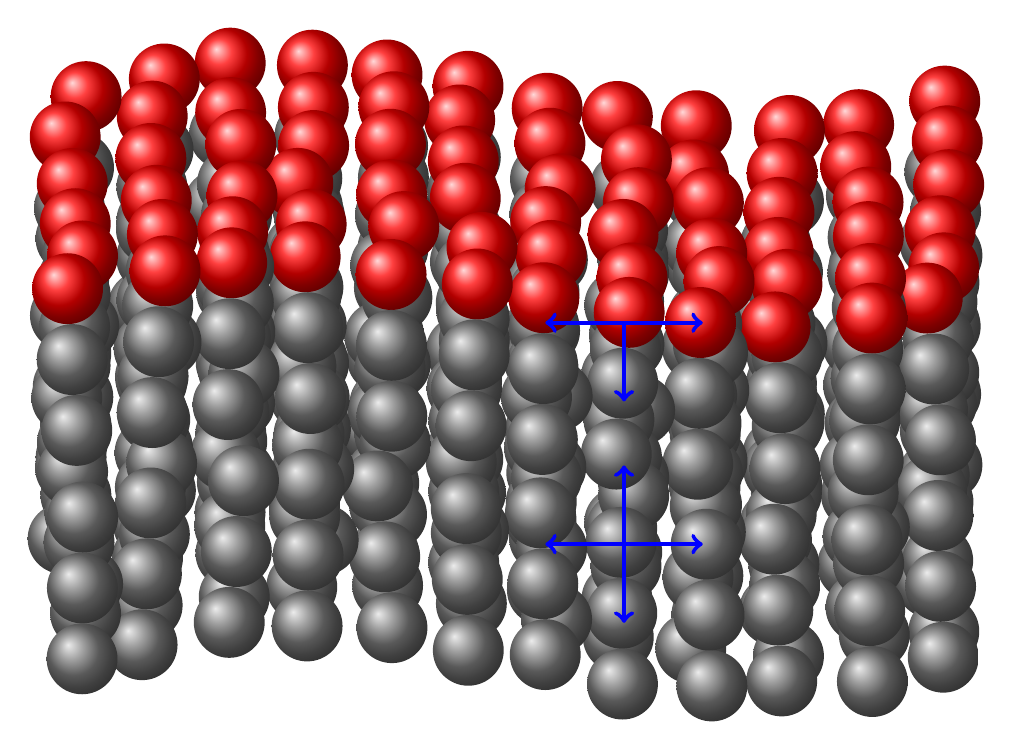
\begin{tikzpicture} 
   
  \def\nuPi{3.1459265}
  \foreach \i in {11,10,...,0}{% This one doesn't matter
    \foreach \j in {5,4,...,0}{% This will crate a membrane
                               % with the front lipids visible
      % top layer
      \pgfmathsetmacro{\dx}{rand*0.1}% A random variance in the x coordinate
      \pgfmathsetmacro{\dy}{rand*0.1}% A random variance in the y coordinate,
                                     % gives a hight fill to the lipid
      \pgfmathsetmacro{\rot}{rand*0.1}% A random variance in the
                                      % molecule orientation      
      \shade[ball color=red] ({\i+\dx+\rot},{0.5*\j+\dy+0.4*sin(\i*\nuPi*10)}) circle(0.45);
      \shade[ball color=gray] (\i+\dx,{0.5*\j+\dy+0.4*sin(\i*\nuPi*10)-0.9}) circle(0.45);
      \shade[ball color=gray] (\i+\dx-\rot,{0.5*\j+\dy+0.4*sin(\i*\nuPi*10)-1.8}) circle(0.45);
      % bottom layer
      \pgfmathsetmacro{\dx}{rand*0.1}
      \pgfmathsetmacro{\dy}{rand*0.1}
      \pgfmathsetmacro{\rot}{rand*0.1}
      \shade[ball color=gray] (\i+\dx+\rot,{0.5*\j+\dy+0.4*sin(\i*\nuPi*10)-2.8}) circle(0.45);
      \shade[ball color=gray] (\i+\dx,{0.5*\j+\dy+0.4*sin(\i*\nuPi*10)-3.7}) circle(0.45);
      \shade[ball color=gray] (\i+\dx-\rot,{0.5*\j+\dy+0.4*sin(\i*\nuPi*10)-4.6}) circle(0.45);
    }
  }
  \draw [ultra thick,blue,<->, shift={(17em,-1em)}] (0,0) -- (2,0) ;
    \draw [ultra thick,blue, ->, shift={(17em,-1em)}] (1,0) -- (1,-1) ;
\begin{scope}[shift={(0em,-9em)}]
  \draw [ultra thick,blue,<->, shift={(17em,0em)}] (0,0) -- (2,0) ;
    \draw [ultra thick,blue, <->, shift={(17em,0em)}] (1,1) -- (1,-1) ;
\end{scope}
  
\end{tikzpicture}}
\begin{tikzpicture} \node[text width=12cm, fontscale=.8, shift={(3em,-10em)}] at (0em,-0em) { \begin{bf}\color{black}\bfseries\large Figure \ref{Fig:{\chapterlabel}\thefigurenewcounter} \end{bf} A representation of surface (red spheres) and bulk (blue spheres) liquid molecules as well as two types of meniscus: a concave and a convex meniscus, typical of water and mercury respectively. Surface molecules are pulled inwards creating the surface tension whereas bulk molecules are not.};
\end{tikzpicture}
  \end{center}
Surface tension values depend on the temperature and the phases in contact and for example the surface tension of the water-air interface is different than the value for the water-mercury interface. The stronger the intermolecular forces, the higher the surface energy--it would take more energy to modify the surface of the liquid. For example, the surface tension of the \ce{C6H6}-air interface (29mN/m) is smaller than the surface tension of the \ce{H2O}-air interface (73mN/m). The surface tension is responsible for phenomena such as the beading of water on the plants leaves--water form beads or drops on the on top of leaves--or the formation of the meniscus, a curved surface of a liquid in a narrow tube. Capillary results from the competitive effect of cohesive and adhesive forces. In the case of mercury, the cohesive forces are stronger than the adhesive and the meniscus created if convex. In the case of water the adhesive forces are stronger and the meniscus is concave.




\refstepcounter{table}  \label{tab:{\chapterlabel}3}
\fontfamily{ppl}\selectfont
\begin{center} \begin{tabular}{llllll}
\rowcolor{black!45}
\toprule
\multicolumn{6}{l}{\hypersetup{colorlinks,linkcolor={white}} \cellcolor{black}\color{white}\bfseries\small Table \ref{tab:{\chapterlabel}3} Surface tension ($\gamma_t$) values for several interfaces at different temperatures.} \\
\midrule
 \rowcolor{gray!10} Interface  &$\gamma_t$ (mN/m)& T &Interface  &$\gamma_t$ (mN/m)& T  \\
\midrule
\ce{H2O}-Air 	&	73& 20$^\circ$C  	&	\ce{H2O}-\ce{Hg} 	&	415& 20$^\circ$C		\\ 
 \ce{CH3I}-Air 	&	67& 20$^\circ$C  	&	\ce{H2O}-Air 	&	73& 22$^\circ$C	\\ 
\ce{C6H6}-Air 	&	30& 20$^\circ$C 	&\ce{H2O}-Air 	&	72& 25$^\circ$C		 \\ 
\ce{CH3OH}-Air 	&	22& 20$^\circ$C & 	\ce{Hg}-Air 	&	486& 20$^\circ$C		\\ 
 \bottomrule
\end{tabular}\end{center} 


   \begin{marginfigure}[0cm]
   \begin{tikzpicture} \node (a) at (0,0) {\includegraphics[width=4cm, height=4cm]{chapter14/figure12}} node[rotate=90, font=\tiny] at ([yshift=.5cm,xshift=.1cm]a.south east) {\textsuperscript{\textcopyright} wikipedia} ;
\node[text width=5cm] at ([yshift=0.2cm]a.north) {\mytriangle{red}Rubbing alcohol has low heat of vaporization};
\end{tikzpicture}
\begin{tikzpicture} \node (a) at (0,0) {\includegraphics[width=4cm, height=4cm]{chapter14/figure13}} node[rotate=90, font=\tiny] at ([yshift=.5cm,xshift=.1cm]a.south east) {\textsuperscript{\textcopyright} Flickr} ;
\node[text width=5cm] at ([yshift=0.2cm]a.north) {\mytriangle{red}Acetone has low heat of vaporization};
\end{tikzpicture}
\begin{tikzpicture} \node (a) at (0,0) {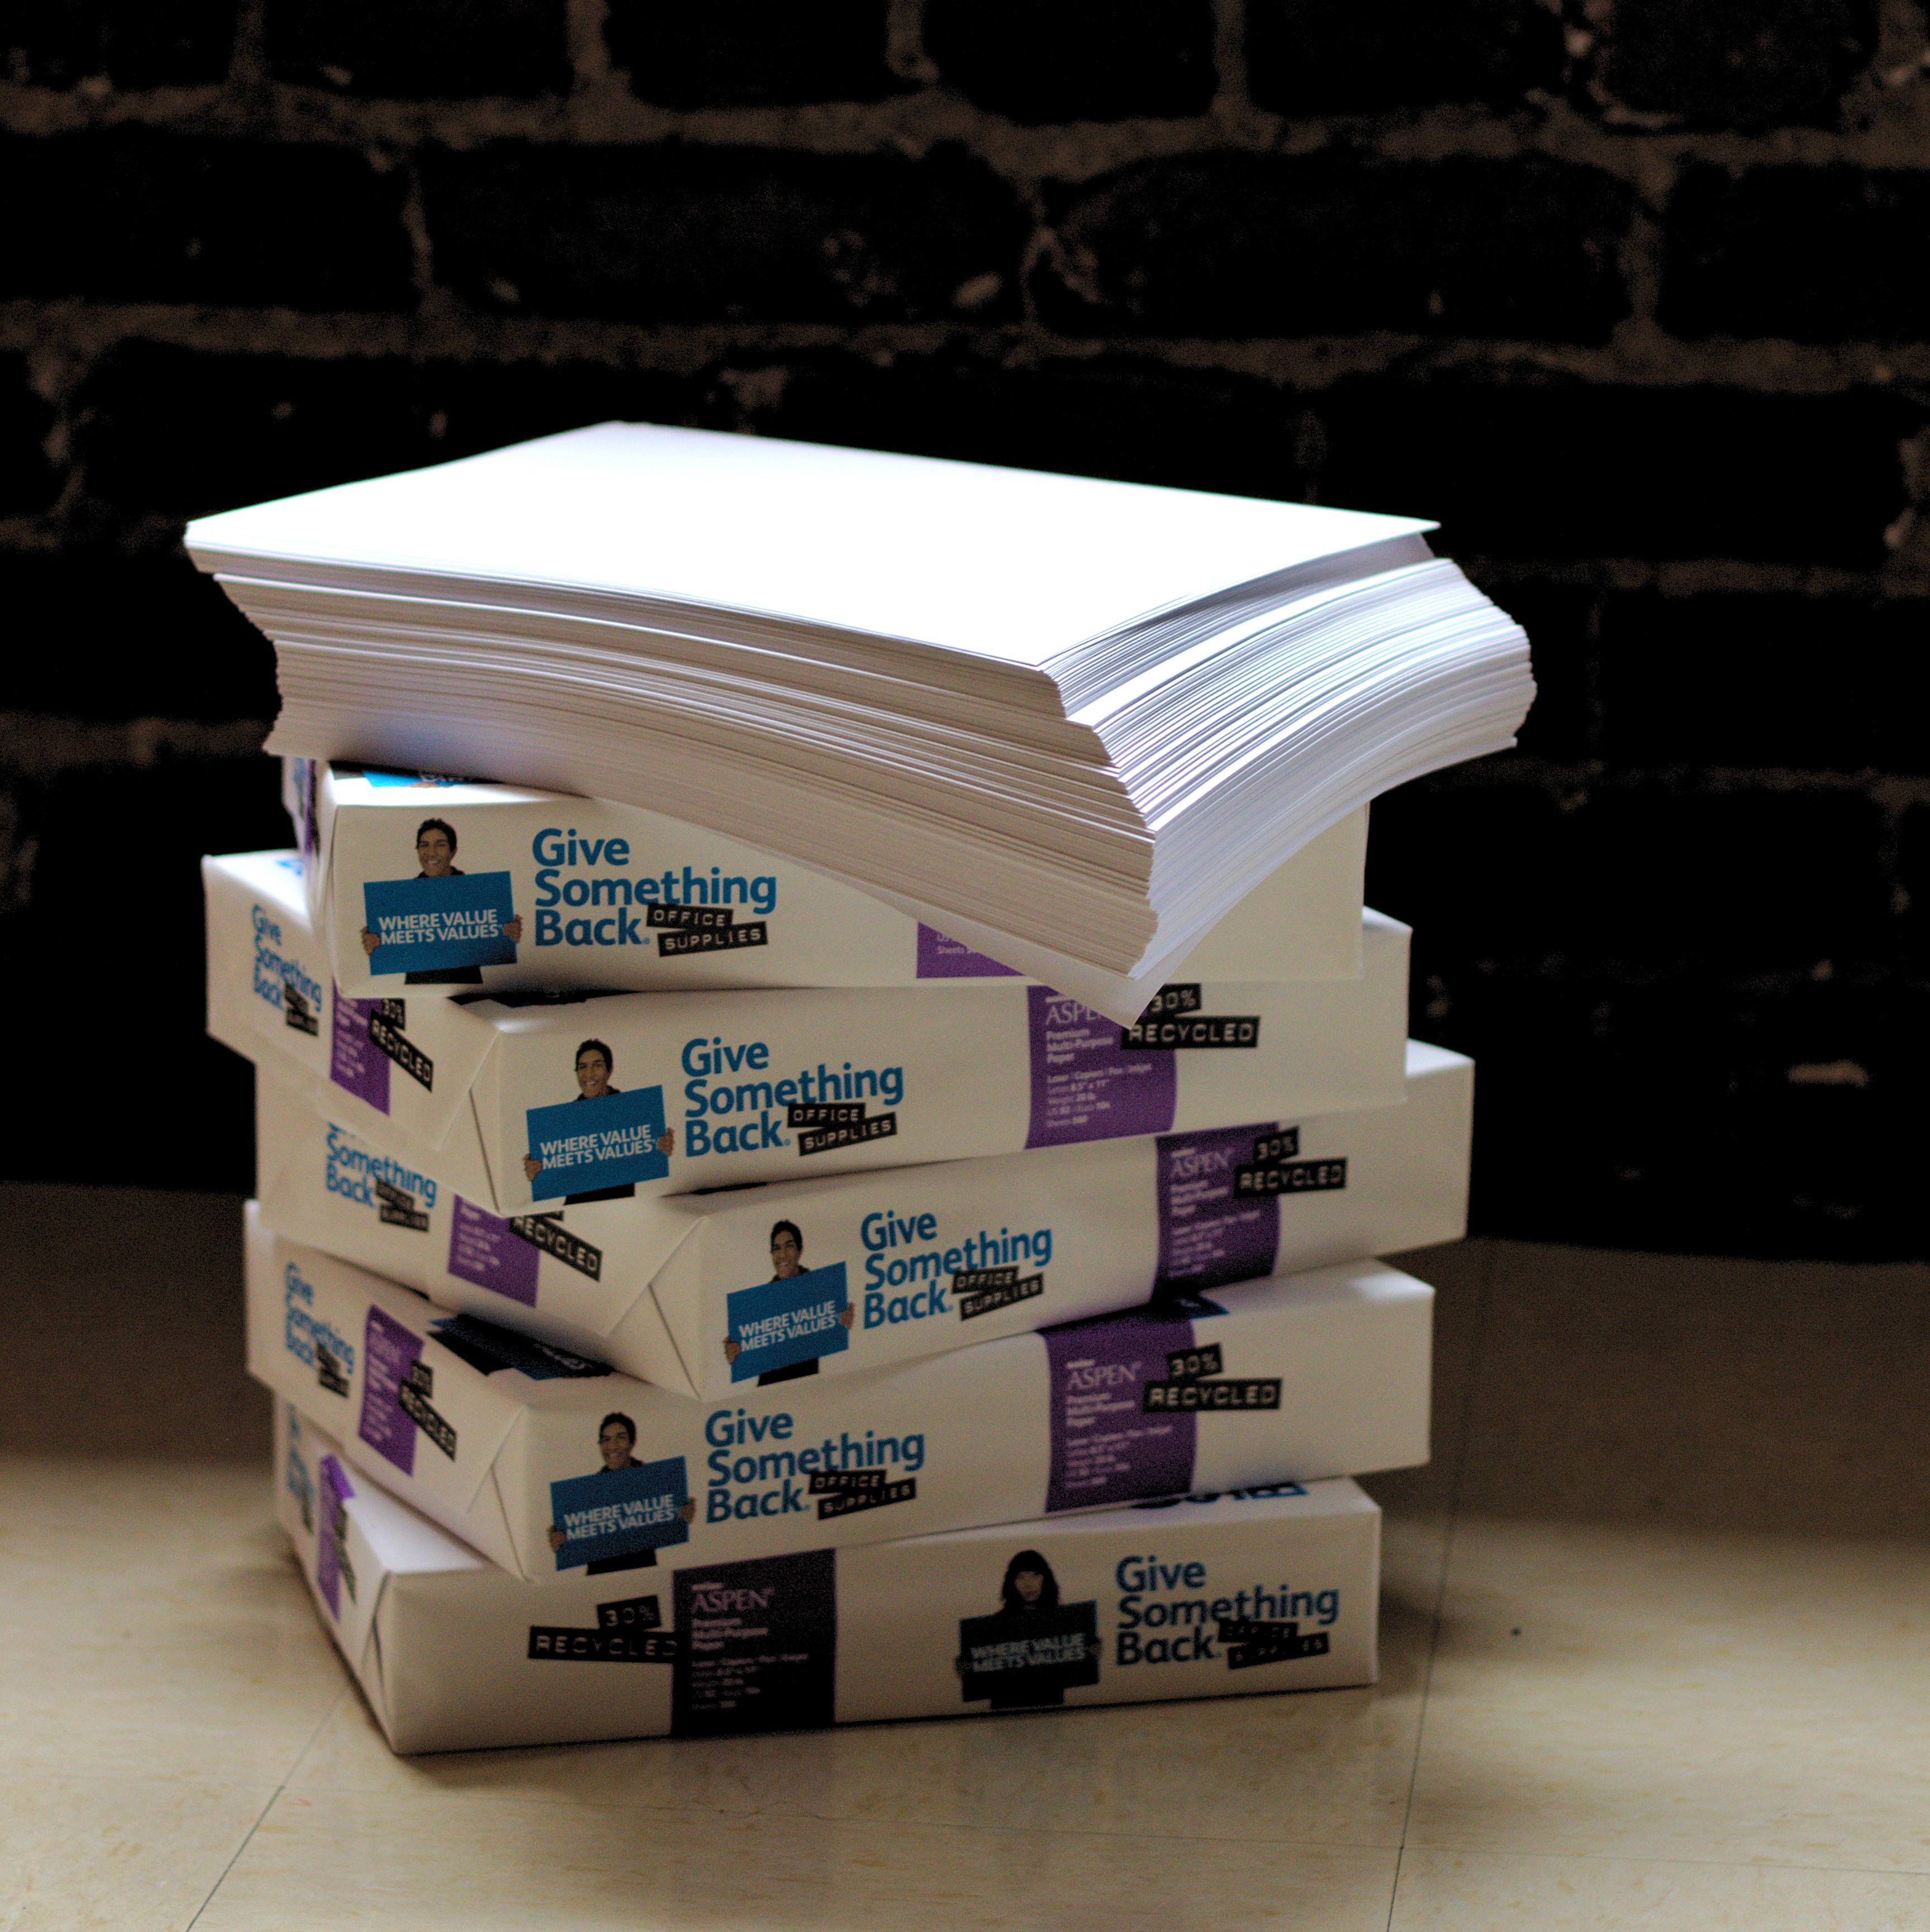
\includegraphics[width=4cm, height=4cm]{chapter14/figure14}} node[rotate=90, font=\tiny] at ([yshift=.5cm,xshift=.1cm]a.south east) {\textsuperscript{\textcopyright} Wikipedia} ;
\node[text width=5cm] at ([yshift=0.2cm]a.north) {\mytriangle{red}Perfumes have low vaporization heat};
\end{tikzpicture}
\begin{tikzpicture} \node (a) at (0,0) {\includegraphics[width=4cm, height=4cm]{chapter14/figure10}} node[rotate=90, font=\tiny] at ([yshift=.5cm,xshift=.1cm]a.south east) {\textsuperscript{\textcopyright} Wikipedia} ;
\node[text width=5cm] at ([yshift=0.2cm]a.north) {\mytriangle{red}Metals have high vaporization heat };
\end{tikzpicture}

%\caption{Some properties of liquids}
%\label{fig:marginfig2}
\end{marginfigure}



\item[\docfilehook{Viscosity}{}]
Viscosity ($\eta$) is the measure of a fluid's resistance to flow. High viscosity liquids flow slowly and this effect results from the intermolecular forces. Liquids with strong intermolecular forces tends to present high viscosities. Viscosity, as well as surface tension, depends on temperature and high temperature reduce the viscosity. Molecular complexity also affect viscosity and long molecules made of carbon and hydrogen have higher viscosities than small molecules due to the fact that because of their size they present more intermolecular interactions. The units of viscosity are milli Pascal-second, mPa$\cdot \text{s}$.
\refstepcounter{table}  \label{tab:{\chapterlabel}4}
\fontfamily{ppl}\selectfont
\begin{center} \begin{tabular}{llllll}
\rowcolor{black!45}
\toprule
\multicolumn{6}{l}{\hypersetup{colorlinks,linkcolor={white}} \cellcolor{black}\color{white}\bfseries\small Table \ref{tab:{\chapterlabel}4} Viscosities ($\eta$) for several substances at different temperatures. } \\
\midrule
  \rowcolor{gray!10} Substance & $\eta$ (mPa$\cdot \text{s}$) &T  &Substance & $\eta$ (mPa$\cdot \text{s}$) &T\\ 
\midrule
Benzene	&0.604&	25$^\circ$C &	Honey &  5000-20000  &  20$^\circ$C\\ 	 
Water&	1.0016&	20$^\circ$C&Pitch &  $2.3\times 10^{11}$  & 10-30$^\circ$C	\\ 
Mercury&	1.526&	25$^\circ$C&	\\ 
Whole milk&	2.12&	20$^\circ$C&	\\ 	 
Olive oil&	56.2&	26$^\circ$C&	\\ 
 \bottomrule
\end{tabular}\end{center} 
\item[\docfilehook{Vapor pressure of a liquid}{}] The molecules of a liquid in contact with the atmosphere are more likely to scape into the gas phase forming what we call the vapor pressure of the liquid. 
When we put a liquid in a closed container, some of the liquid molecules would go into the gas. This process is called vaporization. Whereas molecules of the gas would also go back to the liquid phase. This process is called condensation. Therefore, vaporization and condensation compete until both processes occur at the same speed and the system reaches what we call as equilibrium. The vapor pressure at this state is called the equilibrium vapor pressure or simple the vapor pressure of the liquid.
This effect is responsible for the humidity the air and the smell of liquid chemicals. Chemicals with high vapor pressure vaporize readily and if they have a smell, one would be able to smell them.
Solids also have vapor pressure--solids also have a smell--as their molecules are also able to scape into a gas phase. 
\refstepcounter{table}  \label{tab:{\chapterlabel}5}
\fontfamily{ppl}\selectfont
\begin{center} \begin{tabular}{llllll}
\rowcolor{black!45}
\toprule
\multicolumn{6}{l}{\hypersetup{colorlinks,linkcolor={white}} \cellcolor{black}\color{white}\bfseries\small Table \ref{tab:{\chapterlabel}5} Vapor pressure (P$^{vap}$) for several substances at different temperatures. } \\
\midrule
  \rowcolor{gray!10} Substance & P$^{vap}$ (mmHg) &T  &Substance & P$^{vap}$ (mmHg) &T\\ 
\midrule
Tungsten	 &		0.75&	3203$^\circ$C	&	Carbon dioxide	&		42753&	20$^\circ$C	\\
Ethylene glycol	 &	3.75&	20$^\circ$C	&	Nitrous oxide 	&	42453	&25$^\circ$C	\\
Water 	& 	17.5&	20$^\circ$C&	Carbonyl sulfide	& 	9412	&	25$^\circ$C		\\
Propanol	& 		18.0&	20$^\circ$C	&	Propane 	 &	7584	&	27$^\circ$C	\\
Ethanol	& 	43.7&	20$^\circ$C	&	Formaldehyde	&	3268&	20$^\circ$C	\\
Acetaldehyde	& 	740&	20$^\circ$C&		Butane	& 	1650&	20$^\circ$C	\\
 \bottomrule
\end{tabular}\end{center}

\item[\docfilehook{Enthalpy of vaporization}{}] The enthalpy of vaporization of a liquid ($\Delta H_{vap}$) is the energy needed to vaporize a liquid. This energy is often called heat of vaporization or molar heat of vaporization. Mind that $\Delta H_{vap}$ values are normally positive. This corresponds to the fact that we have to give energy to the liquid in order to create a vapor, and hence the process is endothermic. In general compounds with small heat of vaporization can vaporize easily. Think about the smell of a perfume you like. Now, think about the smell of water. Why a perfume smells and water does not. The enthalpy of vaporization of a perfume is small whereas  $\Delta H_{vap}$ for water is larger (41kJ/mol). This means it is easier for the perfume molecules to scape into the gas phase and hence produce a smell. Another example is acetone--nail polish remover. This chemical has a very distinctive smell. $\Delta H_{vap}$ for acetone is 31kJ/mol. If you compare this value with the value of water you can see acetone is more likely to have a smell. 

\refstepcounter{table}  \label{tab:{\chapterlabel}6}
\fontfamily{ppl}\selectfont
\begin{center} \begin{tabular}{llllll}
\rowcolor{black!45}
\toprule
\multicolumn{6}{l}{\hypersetup{colorlinks,linkcolor={white}} \cellcolor{black}\color{white}\bfseries\small Table \ref{tab:{\chapterlabel}6} Enthalpy of vaporization ($\Delta H_{vap}$) for several substances and boiling points. } \\
\midrule
  \rowcolor{gray!10} Substance &  T&$\Delta H_{vap}$  (J/mol)  &Substance &T &$\Delta H_{vap}$  (J/mol)\\ 
\midrule
Acetone&			56$^\circ$C 	&					31300&	Water&			100$^\circ$C 	&						40660\\	
Aluminium	&	2519$^\circ$C &					294000&		Phosphine&		-88$^\circ$C &					14600\\
Ammonia&		-33$^\circ$C&						23350&		Propane&			-42$^\circ$C 	&				15700\\
Butane&			-1$^\circ$C 		&					21000&		Methanol&		 64.7$^\circ$C	&	 			35200\\
Ethanol	&		78 $^\circ$C &					38600&		Isopropyl alcohol	&	 83$^\circ$C&					44000\\
Hydrogen &		-253$^\circ$C	&		899.2	&	Iron	& 2862$^\circ$C &						340000\\
 \bottomrule
\end{tabular}\end{center}












%\begin{example} %%%%%%%%%%%%%%%%%%%%%%%% EXAMPLE BOX
%Order the following compounds from high to low vapor pressure: \ce{C6H6} ($\Delta H_{vap}$=31kJ/mol), \ce{C6H5OH} ($\Delta H_{vap}$=39kJ/mol), \ce{H2O} ($\Delta H_{vap}$=41kJ/mol)
%\\
%\textlcsc{ \textcolor{dgreen}{\Large \textbf{Solution}} }\\
%The larger $\Delta H_{vap}$ the harder it is to vaporize a liquid and hence the lower the vapor pressure of the liquid. If we compare the liquids in this example, water has the lowest vapor pressure, whereas cyclohexane (\ce{C6H6}) has the highest vapor pressure.
%\\
%\faDiamond\ \textlcsc{ \textcolor{dgreen}{\Large \textbf{Study Check}} }\\
%Order the following compounds from high to low vapor pressure ($P^{vap}$): \ce{NH3} ($\Delta H_{vap}$=23kJ/mol), \ce{CH4} ($\Delta H_{vap}$=8kJ/mol), \ce{C4H10} ($\Delta H_{vap}$=15kJ/mol)
%\begin{flushright} Answer: $P^{vap}(\ce{CH4})$ > $P^{vap}(\ce{C4H10})$ > $P^{vap}(\ce{NH3})$.   \end{flushright}
%\end{example}%%%%%%%%%%%%%%%%%%%%%%%% EXAMPLE BOX


\item[\docfilehook{Vapor pressure change with temperature}{}] 
This vapor pressure strongly depends on temperature. That is the reason why summer days can also be humid days if you live near the seaside. In particular, this change depends on the value of the heat of vaporization. The reason for this, is because at higher temperature more molecules have enough kinetic energy to scape from the liquid into the gas phase. For chemicals with low heat of vaporization we can expect a more sharp change of the vapor pressure with temperature.




\stepcounter{figurenewcounter}   \refstepcounter{figure}  \label{Fig:{\chapterlabel}\thefigurenewcounter}
     \begin{center}
\begin{tikzpicture}
\begin{axis}[
xmin = 10, xmax = 100,
%ymin = -1.5, ymax = 2.0,
%xtick distance = 2.5,
%ytick distance = 0.5,
%grid = both,
minor tick num = 1,
major grid style = {lightgray},
minor grid style = {lightgray!25},
width = \textwidth,
height = 0.5\textwidth,
xlabel = {Temperature ($^\circ$C)},
ylabel = {$P^{vap}$ (mmHg)},
]

 
\addplot[
smooth,
thin,
red,
solid
] file[skip first] {chapter14/data1.dat};
\addplot[
smooth,
thin,
blue,
solid
] file[skip first] {chapter14/data2.dat};
\addplot[
smooth,
thin,
green,
solid
] file[skip first] {chapter14/data3.dat};
%\legend{Benzene,Water}
\draw  (axis cs:25,1000)  node[right, green] {Acetone, $\Delta H_{vap}$=31kJ/mol };
\draw  (axis cs:60,700)  node[right, red] {Benzene, $\Delta H_{vap}$=34kJ/mol };
\draw  (axis cs:60,30)  node[right, blue] {Water, $\Delta H_{vap}$=41kJ/mol };

\end{axis}
\node[text width=12cm, fontscale=.3, shift={(15em,-5em)}] at (0em,0em) { \begin{bf}\color{black}\bfseries\large Figure \ref{Fig:{\chapterlabel}\thefigurenewcounter} \end{bf} Vapor pressure change with temperature for three chemicals with different heat of vaporization.  };

\end{tikzpicture}\end{center}


The following formula gives the relation between vapor pressure and temperature. Mind that for every temperature we will have a vapor pressure value. In the formula you will to pairs of temperatures and hence two pairs of vapor pressures: 

%\resizeableyellownote{2.5}{1}{Add this formula to your flashcard.}
\begin{equation*}
\boxed{  Ln\Bigg(\frac{P^{vap}_{T_1} }{P^{vap}_{T_2}}\Bigg)=\frac{\Delta H_{vap}}{R}\Bigg(\frac{1}{T_2}-\frac{1}{T_1}\Bigg)  } \quad \textcolor{blue}{\text{Clausius-Clapeyron relation}}
\end{equation*}
where:
\begin{where}
 \item $P^{vap}_{T_1}$  is the vapor pressure at temperature $T_1$ in Kelvin
 \item $P^{vap}_{T_2}$  is the vapor pressure at temperature $T_2$ in Kelvin
  \item $\Delta H_{vap}$ is the enthalpy of vaporization in $J\cdot mol^{-1}$
  \item $R$=8.314J$\cdot K^{-1} mol^{-1}$ is the constant of the gases in energy units
\end{where}



\begin{example} %%%%%%%%%%%%%%%%%%%%%%%% EXAMPLE BOX
The vapor pressure of water at 298K is 0.03 atm. Calculate the vapor pressure of water at 323K given $\Delta H_{vap}=43.9 KJ\cdot mol^{-1}$.
\\
\textlcsc{ \textcolor{dgreen}{\Large \textbf{Solution}} }\\
In order to use the Clausius-Clapeyron relation we need two pairs of ($T$, $P^{vap}$) values. In this problem, we have the value of the vapor pressure at 298K, hence we have (298K, 0.03 atm) and they ask the pressure at 323K. Therefore the second pair is  (298K, x atm), where X is the vapor pressure at 298--what they are asking in the problem. We can call (298K, 0.03 atm) as ($T_1$, $P^{vap}_{T_1}$) and (298K, X atm) as ($T_2$, $P^{vap}_{T_2}$). At this point we have $T_1=298K$ and $P^{vap}_{T_1}=0.03 atm$ and $T_2=323K$ and $P^{vap}_{T_2}=x$. We also have the enthalpy of vaporization. Minds that this value has to be given in $J\cdot mol^{-1}$ and hence, we will use $\Delta H_{vap}=43.9\times 10^3J\cdot mol^{-1}$. Now we can plug these values into the formula:
\begin{equation*}
Ln\Bigg(\frac{0.03 }{x}\Bigg)=\frac{43.9\times 10^3}{8.314}\Bigg(\frac{1}{323}-\frac{1}{298}\Bigg)  
\end{equation*}
Let us solve this step by step. First we solve the part on the right:
\begin{equation*}
Ln\Bigg(\frac{0.03} {x}\Bigg)=-1.37
\end{equation*}
Now, in order to eliminate the logarithm we should use the exponential function in both sides:
\begin{equation*}\frac{0.03} {x}=\myexp{-1.37}\end{equation*}
Calculating the exponential of -1.37 we have:
\begin{equation*}\frac{0.03} {x}=0.25\end{equation*}
That leads to a x value of 0.12 atm.
\\
\faDiamond\ \textlcsc{ \textcolor{dgreen}{\Large \textbf{Study Check}} }\\
Using the data below, calculate $\Delta H_{vap}$ for \ce{HNO3}.\\
\begin{tabularx}{\textwidth}{YY}
  \toprule
 T (K)& $P^{vap}$ (mmHg)   \\
    \midrule
  10 & 	 26.6		   \\
    20 & 	 47.9		   \\
      30 & 	81.3		   \\
    \bottomrule
\end{tabularx}
\begin{flushright} Answer: 97.80 J/mol.   \end{flushright}
\end{example}%%%%%%%%%%%%%%%%%%%%%%%% EXAMPLE BOX

\end{description}






\section{Phase diagrams}
Water can be found at different states: liquid, solid and gas. We know at room temperature--and atmospheric pressure--water is a liquid. However, what if we warm up a sample of water? When does it become vapor? And more importantly, what if the working pressure is not one atmosphere? Would water boil the same near the sea or on top of a mountain? The answer to all these questions can be found in the phase diagram of water. This section will cover phase diagrams. You will learn how to read phase diagrams in order to predict the state of matter at any temperature and pressure conditions. You will also learn how to identify critical and triple points.

\stepcounter{figurenewcounter}   \refstepcounter{figure}  \label{Fig:{\chapterlabel}\thefigurenewcounter}
     \begin{center}
\begin{tikzpicture}[scale=1]
\pgfmathsetmacro{\TPX}{1.5}
\pgfmathsetmacro{\TPY}{5}
\pgfmathsetmacro{\CPX}{2.5}
\pgfmathsetmacro{\CPY}{50}
\pgfmathsetmacro{\TOPX}{2}
\pgfmathsetmacro{\TOPY}{100}
\pgfmathsetmacro{\XMIN}{0}
\pgfmathsetmacro{\XMAX}{3}
\pgfmathsetmacro{\YMIN}{1}
\pgfmathsetmacro{\YMAX}{100}
\begin{semilogyaxis}[xmin=\XMIN,ymin=\YMIN,xmax=\XMAX,ymax=\YMAX,axis on top, xticklabels={}, yticklabels={}, xlabel={Temperature },ylabel={Pressure }, ticks=none]
\draw [blue, fill=blue]  (\TPX,\TPY) to (\TOPX,\TOPY)  to (\CPX,\TOPY) to (\CPX,\CPY) to [bend left] (\TPX,\TPY);

%\addplot[name path=gas,very thick, bend right=70] coordinates {(0,1) (1,10) (2,32)};
\addplot[name path=liq,very thick] coordinates {(\TPX,\TPY) (\TOPX,\TOPY) (\CPX,\TOPY)};
%\addplot[name path=help1] coordinates {(2,100) (0,100) (0,1)};
\addplot[name path=help2] coordinates {(\XMIN,\YMIN) (\XMAX,\YMIN) (\XMAX,\CPY)};
\draw[name path=gas,very thick ](\XMIN,1) to [bend right] (\TPX,\TPY) to [bend right] (\CPX,\CPY);
\draw[name path=gas3 ] (\TPX,\TPY) to [bend right] (\CPX,\CPY);
\draw[name path=liq2 ](\XMIN,1) to [bend right] (\TPX,\TPY) node [below, xshift=2cm, white] {Gas}  node [below, yshift=2cm, xshift=-2cm, white] {Solid} node [yshift=2cm, xshift=2cm, white] {Liquid};
\addplot[name path=help11] coordinates {(\TPX,\TPY) (\TOPX,\YMAX) (\XMIN,\YMAX) (\XMIN,\YMIN)};
%\addplot[green] fill between[of=liq2 and help11];

\draw[fill=green ](\XMIN,1) to [bend right] (\TPX,\TPY) -- (\TPX,\TPY)  --(\TOPX,\YMAX) --(\XMIN,\YMAX)  --(\XMIN,\YMIN)  ;
\draw[name path=liq2 ](\XMIN,1) to [bend right] (\TPX,\TPY) node [below, xshift=2cm, white] {Gas}  node [below, yshift=2cm, xshift=-2cm, white] {Solid} node [yshift=2cm, xshift=2cm, white] {Liquid};



\addplot[red] fill between[of=gas and help2];
\shade[shading=azimuth,vcol=blue,hcol=red] (axis cs:\CPX,\CPY) rectangle (axis cs:\XMAX,\YMAX);
%\draw (\TPX,\TPY) node[above,white, xshift=0.2cm] {TP};
%\draw (\CPX,\CPY) node[above,white] {CP};
%\draw[white, dashed, thick]  (0,\TPY)  node [xshift=0.5cm, yshift=0.2cm ]  {\small 0.0006} -- (\TPX,\TPY) -- (\TPX,\YMIN) node [yshift=0.2cm,xshift=0.5cm ] {\small 0.0098};
%\draw[white, dashed, thick]  (0,\CPY)  node [xshift=0.5cm, yshift=0.2cm ]  {\small 218} -- (\CPX,\CPY) -- (\CPX,\YMIN) node [yshift=0.2cm,xshift=0.5cm ] {\small 374};
%\draw[thick,o-stealth, white] (1,20) node [xshift=-0.5cm, yshift=0.3cm ]  {\small (000, 218)} -- (2,20) node [xshift=0.5cm, yshift=0.3cm ]  {\small (000, 218)};
%\draw[white] (\TPX,\TPY) node {\small TP} node [xshift=-0.5cm, yshift=-0.3cm ]  {\tiny (0.0098 C$^{\circ}$, 0.006 atm)};
%\draw[white] (\CPX,\CPY) node {\small CP} node [xshift=-0.5cm, yshift=-0.3cm ]  {\tiny (374 C$^{\circ}$, 218 atm)};
\end{semilogyaxis}
\draw[color=black,fill=black, shift={(15.3em,5.5em)}] (0,0) circle [radius=0.07] node[color=white,shift={(1em,-0.5em)}] {\tiny Triple point};
\draw[color=black,fill=black, shift={(25.2em,13.2em)}] (0,0) circle [radius=0.07] node[color=white,shift={(1.5em,-0.5em)}] {\tiny Critical point};
\node[text width=12cm, fontscale=.3, shift={(15em,-6em)}] at (0em,0em) { \begin{bf}\color{black}\bfseries\large Figure \ref{Fig:{\chapterlabel}\thefigurenewcounter} \end{bf}A typical phase diagram showing the different phases, the critical and the triple point. As the slope of the line that separates liquid and gas has an angle lower than 90$^{\circ}$ the solid phase has higher density that the liquid. };

\end{tikzpicture}\end{center}
\sloppy 
\begin{description}
\item[\docfilehook{Description of a phase diagram: important points}{}] 
A phase diagram is a representation of the different temperature and pressure conditions in which we can find the different states of matter of a substance. Normally, temperature is listed in the horizontal axis and pressure in the vertical axis. The different phase, liquid, solid and gas, are listed. At low temperature we tend to find solids and gases are common at high temperature. Similarly, at low pressures we tend to find gases and solids at high pressure. With pressure we refer to compressive pressure. 
The lines in a phase diagram represent equilibrium and the line separating solid and gas represents all the pressure and temperature conditions in which we can find a gas in equilibrium with a liquid. Similarly, the line separating liquid and solid represents all the pressure and temperature conditions in which we can find a liquid in equilibrium with a solid. With equilibrium, we mean that both phase are present and the process of phase transition proceeds at the same speed in both directions.There are two important points in a phase diagram: the critical point and the triple point. The triple point is the pressure and temperature conditions in which the three phases--solid, liquid and gas--coexist. Another important point is the critical point. Beyond this point one cannot liquefy (go from gas into a liquid) or condense (go from liquid into a gas) the substance. 
There is one more important feature one can extract from a phase diagram. Normally, but  not always, solids are more dense than liquids. We can compare the density of the solid and the liquid by analyzing the slope of the line connecting both phase. If the slope is lower than 90$^{\circ}$ then the solid will be more dense than the liquid. If it is larger than 90$^{\circ}$ then the solid is less dense than the liquid. If the slope is 90$^{\circ}$ then both liquid and solid have the same density.



\item[\docfilehook{What are normal conditions?}{}] When we speak about normal conditions we refer to a pressure of 1atm, which is the common atmospheric pressure. But remember that the atmospheric pressure depends on the height of the location where measured. And locations near the see--at low height--tend to have higher pressure than locations near the mountains--at a larger height.
\item[\docfilehook{Phase transition terminology}{}]
Each phase transition has a specific name. You may be familiar with some of the terms like freezing that involves the change from liquid to solid. Other names are listed below:
\begin{center}Liquid \ce{->} Solid \hspace*{0pt}\hfill Freezing\\
Liquid\ce{->} Gas \hspace*{0pt}\hfill Evaporation or vaporization\\
Solid\ce{->} Liquid \hspace*{0pt}\hfill Melting\\
Gas \ce{->} Liquid \hspace*{0pt}\hfill Condensation\\
Solid \ce{->} Gas \hspace*{0pt}\hfill Sublimation\\
Gas or Solid \ce{->} Liquid \hspace*{0pt}\hfill Liquefy 

\end{center}
\stepcounter{figurenewcounter}   \refstepcounter{figure}  \label{Fig:{\chapterlabel}\thefigurenewcounter}
     \begin{center}
\begin{tikzpicture}
\pgfmathsetmacro{\TPX}{1.5}
\pgfmathsetmacro{\TPY}{5}
\pgfmathsetmacro{\CPX}{2.5}
\pgfmathsetmacro{\CPY}{50}
\pgfmathsetmacro{\TOPX}{1}
\pgfmathsetmacro{\TOPY}{100}
\pgfmathsetmacro{\XMIN}{0}
\pgfmathsetmacro{\XMAX}{3}
\pgfmathsetmacro{\YMIN}{1}
\pgfmathsetmacro{\YMAX}{100}
\begin{semilogyaxis}[xmin=\XMIN,ymin=\YMIN,xmax=\XMAX,ymax=\YMAX,axis on top, xticklabels={}, yticklabels={}, xlabel={Temperature in Celsius},ylabel={Pressure in atm}, ticks=none]
\draw [blue, fill=blue]  (\TPX,\TPY) to (\TOPX,\TOPY)  to (\CPX,\TOPY) to (\CPX,\CPY) to [bend left] (\TPX,\TPY);

%\addplot[name path=gas,very thick, bend right=70] coordinates {(0,1) (1,10) (2,32)};
\addplot[name path=liq,very thick] coordinates {(\TPX,\TPY) (\TOPX,\TOPY) (\CPX,\TOPY)};
%\addplot[name path=help1] coordinates {(2,100) (0,100) (0,1)};
\addplot[name path=help2] coordinates {(\XMIN,\YMIN) (\XMAX,\YMIN) (\XMAX,\CPY)};
\draw[name path=gas,very thick ](\XMIN,1) to [bend right] (\TPX,\TPY) to [bend right] (\CPX,\CPY);
\draw[name path=gas3 ] (\TPX,\TPY) to [bend right] (\CPX,\CPY);
\draw[name path=liq2 ](\XMIN,1) to [bend right] (\TPX,\TPY) node [below, xshift=2cm, white] {Gas}  node [below, yshift=2cm, xshift=-2cm, white] {Solid} node [yshift=2cm, xshift=2cm, white] {Liquid};
\addplot[name path=help11] coordinates {(\TPX,\TPY) (\TOPX,\YMAX) (\XMIN,\YMAX) (\XMIN,\YMIN)};
\addplot[green] fill between[of=liq2 and help11];
\addplot[red] fill between[of=gas and help2];
\shade[shading=azimuth,vcol=blue,hcol=red] (axis cs:\CPX,\CPY) rectangle (axis cs:\XMAX,\YMAX);
%\draw (\TPX,\TPY) node[above,white, xshift=0.2cm] {TP};
%\draw (\CPX,\CPY) node[above,white] {CP};
%\draw[white, dashed, thick]  (0,\TPY)  node [xshift=0.5cm, yshift=0.2cm ]  {\small 0.0006} -- (\TPX,\TPY) -- (\TPX,\YMIN) node [yshift=0.2cm,xshift=0.5cm ] {\small 0.0098};
%\draw[white, dashed, thick]  (0,\CPY)  node [xshift=0.5cm, yshift=0.2cm ]  {\small 218} -- (\CPX,\CPY) -- (\CPX,\YMIN) node [yshift=0.2cm,xshift=0.5cm ] {\small 374};
%\draw[thick,o-stealth, white] (1,20) node [xshift=-0.5cm, yshift=0.3cm ]  {\small (000, 218)} -- (2,20) node [xshift=0.5cm, yshift=0.3cm ]  {\small (000, 218)};
%\draw[white] (\TPX,\TPY) node {\small TP} node [xshift=-0.5cm, yshift=-0.3cm ]  {\tiny (0.0098 C$^{\circ}$, 0.006 atm)};
%\draw[white] (\CPX,\CPY) node {\small CP} node [xshift=-0.5cm, yshift=-0.3cm ]  {\tiny (374 C$^{\circ}$, 218 atm)};
\draw[white, dashed, thick]  (0,15)  node [xshift=0.5cm, yshift=0.2cm ]  {\small 1 atm} -- (1.7,15) -- (1.7,\YMIN) node [yshift=0.2cm,xshift=0.5cm ] {\small 25 C$^{\circ}$};
\end{semilogyaxis}

\node[text width=12cm, fontscale=.3, shift={(15em,-6em)}] at (0em,0em) { \begin{bf}\color{black}\bfseries\large Figure \ref{Fig:{\chapterlabel}\thefigurenewcounter} \end{bf} The phase diagram of water with pressure in the Y axis and temperature in the X axis. This diagram displays the different states of matter of water for different pressure and temperature conditions. The coordinated of the triple point are (0.0098 C$^{\circ}$,0.0060 atm). This means that at this low pressure and temperature conditions we have three phases in contact: water, ice and steam. The coordinates of the critical point are (374 C$^{\circ}$, 218 atm). This means that for temperature beyond 374 C$^{\circ}$ it is not possible to liquefy steam. };

\end{tikzpicture}\end{center}


\item[\docfilehook{Phase diagram of water}{}] A phase diagram is just a diagram with temperature in the X axis and pressure in the Y axis. It tells you whether you have gas, liquid or gas at a large range of pressure and temperature conditions. For example, the figure on the side of the page presents the phase diagram of water and the line indicates the phase present at (Temperature, Pressure) conditions of (25 C$^{\circ}$,1 atm). Obviously, this phase is liquid water. \emph{Normal conditions} refer to pressure conditions of 1 atm. Hence, we say that the normal boiling point of water--this means at 1 atm--is 100 C$^{\circ}$. In the following we will analyze a set of experiments represented as vertical and horizontal lines in the diagram. Horizontal lines are cooling/heating experiments in which pressure is kept fixed and temperature changes. Vertical lines represent compression/decompression experiments in which pressure changes at constant temperature.




\item[\docfilehook{Heating and compression experiments}{}] 
We will analyze now some cooling/heating experiments. In the first experiment, we start by having a solid that we  heat up to obtain first a mixture between liquid and solid and then a pure liquid. In this experiment we just transitioned between solid into a liquid. Experiment 2 is different. We also start by having a solid. The difference is that this time we reach a point called \emph{tripe point} in this point the three phase coexist at a single pressure and temperature. Therefore, in this experiment, we go from a solid into a mixture of solid, liquid and gas. After that we transition directly into a gas. Experiment number three is called sublimation. In this experiment we start by having a solid that transitions into a gas by means of a mixture of solid and gas. We can also discuss some compression/decompression experiments. The first experiment is a compression experiment in which we start from a gas and we end up having a liquid by means of a mixture of both. The second experiment start beyond the \emph{critical point} and hence even if you compress the gas you will never reach a liquid state. The critical point is the point beyond which one cannot liquefy a gas or gasify a liquid.

\vspace{4cm}
\stepcounter{figurenewcounter}   \refstepcounter{figure}  \label{Fig:{\chapterlabel}\thefigurenewcounter}
     \begin{center}
\begin{tikzpicture}
\begin{scope}[transform canvas={scale=.6},overlay]
\pgfmathsetmacro{\TPX}{1.5}
\pgfmathsetmacro{\TPY}{5}
\pgfmathsetmacro{\CPX}{2.5}
\pgfmathsetmacro{\CPY}{50}
\pgfmathsetmacro{\TOPX}{1}
\pgfmathsetmacro{\TOPY}{100}
\pgfmathsetmacro{\XMIN}{0}
\pgfmathsetmacro{\XMAX}{3}
\pgfmathsetmacro{\YMIN}{1}
\pgfmathsetmacro{\YMAX}{100}
\begin{semilogyaxis}[xmin=\XMIN,ymin=\YMIN,xmax=\XMAX,ymax=\YMAX,axis on top, xticklabels={}, yticklabels={}, xlabel={\Large Temperature},ylabel={\Large Pressure}, x=3.0cm, y=1.5cm, ticks=none]
%\draw [blue, fill=blue]  (\TPX,\TPY) to (\TOPX,\TOPY)  to (\CPX,\TOPY) to (\CPX,\CPY) to [bend left] (\TPX,\TPY);
%\addplot[name path=gas,very thick, bend right=70] coordinates {(0,1) (1,10) (2,32)};
\addplot[name path=liq,very thick] coordinates {(\TPX,\TPY) (\TOPX,\TOPY) (\CPX,\TOPY)};
%\addplot[name path=help1] coordinates {(2,100) (0,100) (0,1)};
\addplot[name path=help2] coordinates {(\XMIN,\YMIN) (\XMAX,\YMIN) (\XMAX,\CPY)};
\draw[name path=gas,very thick ](\XMIN,1) to [bend right] (\TPX,\TPY) to [bend right] (\CPX,\CPY);
\draw[name path=gas3 ] (\TPX,\TPY) to [bend right] (\CPX,\CPY);
\draw[name path=liq2 ](\XMIN,1) to [bend right] (\TPX,\TPY) node [below, xshift=2cm, yshift=-1cm, black] {\Large G}  node [below, yshift=3cm, xshift=-4cm, black] {\Large S} node [yshift=2cm, xshift=2cm, black] {\Large L};
\addplot[name path=help11] coordinates {(\TPX,\TPY) (\TOPX,\YMAX) (\XMIN,\YMAX) (\XMIN,\YMIN)};
%\addplot[green] fill between[of=liq2 and help11];
%\addplot[red] fill between[of=gas and help2];
%\shade[shading=azimuth,vcol=blue,hcol=red] (axis cs:\CPX,\CPY) rectangle (axis cs:\XMAX,\YMAX);
%\draw (\TPX,\TPY) node[above,white, xshift=0.2cm] {TP};
%\draw (\CPX,\CPY) node[above,white] {CP};
%\draw[white, dashed, thick]  (0,\TPY)  node [xshift=0.5cm, yshift=0.2cm ]  {\small 0.0006} -- (\TPX,\TPY) -- (\TPX,\YMIN) node [yshift=0.2cm,xshift=0.5cm ] {\small 0.0098};
%\draw[white, dashed, thick]  (0,\CPY)  node [xshift=0.5cm, yshift=0.2cm ]  {\small 218} -- (\CPX,\CPY) -- (\CPX,\YMIN) node [yshift=0.2cm,xshift=0.5cm ] {\small 374};
\draw[thick,o-stealth, black, dashed] (1,20) node [xshift=-0.5cm, yshift=0.0cm ]  {\small EXP 1} -- (1.5,20) ;
\draw[thick,o-stealth, black, dashed] (0.5,\TPY) node [xshift=-0.5cm, yshift=0.0cm ]  {\small EXP 2} -- (2,\TPY) ;
\draw[thick,o-stealth, black, dashed] (0.5,2) node [xshift=-0.5cm, yshift=0.0cm ]  {\small EXP 3} -- (1.5,2) ;

%\draw[white] (\TPX,\TPY) node {\small TP} node [xshift=-0.5cm, yshift=-0.3cm ]  {\tiny (0.0098 C$^{\circ}$, 0.006 atm)};
%\draw[white] (\CPX,\CPY) node {\small CP} node [xshift=-0.5cm, yshift=-0.3cm ]  {\tiny (374 C$^{\circ}$, 218 atm)};
\end{semilogyaxis}
\end{scope}



\begin{scope}[shift={(30em,0em)},transform canvas={scale=.6},overlay]
\pgfmathsetmacro{\TPX}{1.5}
\pgfmathsetmacro{\TPY}{5}
\pgfmathsetmacro{\CPX}{2.5}
\pgfmathsetmacro{\CPY}{50}
\pgfmathsetmacro{\TOPX}{1}
\pgfmathsetmacro{\TOPY}{100}
\pgfmathsetmacro{\XMIN}{0}
\pgfmathsetmacro{\XMAX}{3}
\pgfmathsetmacro{\YMIN}{1}
\pgfmathsetmacro{\YMAX}{100}
\begin{semilogyaxis}[xmin=\XMIN,ymin=\YMIN,xmax=\XMAX,ymax=\YMAX,axis on top, xticklabels={}, yticklabels={}, xlabel={\Large Temperature},ylabel={\Large Pressure}, x=3.0cm, y=1.5cm, ticks=none]
%\draw [blue, fill=blue]  (\TPX,\TPY) to (\TOPX,\TOPY)  to (\CPX,\TOPY) to (\CPX,\CPY) to [bend left] (\TPX,\TPY);
%\addplot[name path=gas,very thick, bend right=70] coordinates {(0,1) (1,10) (2,32)};
\addplot[name path=liq,very thick] coordinates {(\TPX,\TPY) (\TOPX,\TOPY) (\CPX,\TOPY)};
%\addplot[name path=help1] coordinates {(2,100) (0,100) (0,1)};
\addplot[name path=help2] coordinates {(\XMIN,\YMIN) (\XMAX,\YMIN) (\XMAX,\CPY)};
\draw[name path=gas,very thick ](\XMIN,1) to [bend right] (\TPX,\TPY) to [bend right] (\CPX,\CPY);
\draw[name path=gas3 ] (\TPX,\TPY) to [bend right] (\CPX,\CPY);
\draw[name path=liq2 ](\XMIN,1) to [bend right] (\TPX,\TPY) node [below, xshift=2cm, yshift=-1cm, black] {\Large G}  node [below, yshift=3cm, xshift=-4cm, black] {\Large S} node [yshift=2cm, xshift=2cm, black] {\Large L};
\addplot[name path=help11] coordinates {(\TPX,\TPY) (\TOPX,\YMAX) (\XMIN,\YMAX) (\XMIN,\YMIN)};
%\addplot[green] fill between[of=liq2 and help11];
%\addplot[red] fill between[of=gas and help2];
%\shade[shading=azimuth,vcol=blue,hcol=red] (axis cs:\CPX,\CPY) rectangle (axis cs:\XMAX,\YMAX);
%\draw (\TPX,\TPY) node[above,white, xshift=0.2cm] {TP};
%\draw (\CPX,\CPY) node[above,white] {CP};
%\draw[white, dashed, thick]  (0,\TPY)  node [xshift=0.5cm, yshift=0.2cm ]  {\small 0.0006} -- (\TPX,\TPY) -- (\TPX,\YMIN) node [yshift=0.2cm,xshift=0.5cm ] {\small 0.0098};
%\draw[white, dashed, thick]  (0,\CPY)  node [xshift=0.5cm, yshift=0.2cm ]  {\small 218} -- (\CPX,\CPY) -- (\CPX,\YMIN) node [yshift=0.2cm,xshift=0.5cm ] {\small 374};
\draw[thick,o-stealth, black, dashed, yshift=-1.3cm] (1,-125)  node [xshift=-0.5cm, yshift=0.0cm ]  {\small EXP 1} -- (1,20) ;
\draw[thick,o-stealth, black, dashed, xshift=5.3cm] (1,-125)  node [xshift=-0.5cm, yshift=0.0cm ]  {\small EXP 2} -- (1,80) ;
%\draw[thick,o-stealth, black, dashed] (0.5,\TPY) node [xshift=-0.5cm, yshift=0.0cm ]  {\small EXP 2} -- (2,\TPY) ;
%\draw[thick,o-stealth, black, dashed] (0.5,2) node [xshift=-0.5cm, yshift=0.0cm ]  {\small EXP 3} -- (1.5,2) ;

%\draw[white] (\TPX,\TPY) node {\small TP} node [xshift=-0.5cm, yshift=-0.3cm ]  {\tiny (0.0098 C$^{\circ}$, 0.006 atm)};
%\draw[white] (\CPX,\CPY) node {\small CP} node [xshift=-0.5cm, yshift=-0.3cm ]  {\tiny (374 C$^{\circ}$, 218 atm)};
\end{semilogyaxis}
\end{scope}
\node[text width=12cm, fontscale=.3, shift={(16em,-3em)}] at (-0em,-0em) { \begin{bf}\color{black}\bfseries\large Figure \ref{Fig:{\chapterlabel}\thefigurenewcounter} \end{bf} Heating experiments  (left) and compression experiments (right). };

\end{tikzpicture}\end{center}



\item[\docfilehook{Energy calculations involving phase transitions}{}] 
The enthalpy of vaporization of a substance gives you the amount of energy needed to vaporize an amount of substance. Similarly, the enthalpy of fusion tells you about the energy involved in the fusion process. Each phase--gas, liquid and vapor--has different specific heat. Using water as an example, imagine we need to calculate the energy involved in the heating of $m$=18grams ($n$=1 mole) of water from 20$^{\circ}$C to a 150$^{\circ}$C. This energy results from three contributions: the energy needed to warm up liquid from 20$^{\circ}$C to a 100$^{\circ}$C (we can call this $\Delta T_1$), the energy to boil 1 mole of water, and the energy to warm up 1 mole of gas water from 100$^{\circ}$C to a 150$^{\circ}$C (we can call this $\Delta T_2$). The final calculation will be:
\begin{equation*}
Q=m\cdot c_e^{\ce{H2O_{(\ell)}}}\cdot \Delta T_1 + n\cdot \Delta H_{vap}^{\ce{H2O}} + m\cdot c_e^{\ce{H2O_{(g)}}}\cdot \Delta T_2
\end{equation*}



\refstepcounter{table}  \label{tab:{\chapterlabel}7}
\fontfamily{ppl}\selectfont
\begin{center} \begin{tabular}{llll}
\rowcolor{black!45}
\toprule
\multicolumn{4}{l}{\hypersetup{colorlinks,linkcolor={white}} \cellcolor{black}\color{white}\bfseries\small Table \ref{tab:{\chapterlabel}7} Properties of the different states of matter of water. } \\
\midrule
  \rowcolor{gray!10} Property & Ice &Water &Steam  \\ 
\midrule
Density (g/mL)	 &	0.93	 &	1 	&	0.6	\\
$c_e$ (J$\cdot g^{-1}\cdot ^{\circ}C^{-1}$)	 &2.18		 &4.184	 	&1.99	 	\\
$\Delta H_{fusion}$ (kJ/mol)	 &\multicolumn{3}{l}{	6.01	 }	 	\\
$\Delta H_{vap}$ (kJ/mol)	 &	\multicolumn{3}{l}{	44	}	 	\\
 \bottomrule
\end{tabular}\end{center}
\end{description}



%
%\begin{asy}
%//[width=2cm] 
%import three;
%size(100);
%int d = 50;
%currentprojection=perspective(300,-650,500,center=true);
%// define two types of ions
%surface iona = scale3(20)*unitsphere;
%surface ionb = scale3(25)*unitsphere;
%// surface properties and color of the ions
%material White = material(diffusepen=gray(0.4),emissivepen=gray(0.6));
%// style of lines connecting ions
%pen thick=linewidth(1);
%draw(shift(d*(1,1,1))*iona,White);
%draw(shift(d*(-1,1,1))*iona,White);
%draw(shift(d*(1,-1,1))*iona,White);
%draw(shift(d*(-1,-1,1))*iona,White);
%draw(shift(d*(1,1,-1))*iona,White);
%draw(shift(d*(-1,1,-1))*iona,White);
%draw(shift(d*(1,-1,-1))*iona,White);
%draw(shift(d*(-1,-1,-1))*iona,White);
%draw(d*(-1,-1,1)--d*(-1,1,1),thick);draw(d*(-1,-1,1)--d*(1,-1,1),thick);draw(d*(1,-1,1)--d*(1,1,1),thick);draw(d*(1,1,1)--d*(-1,1,1),thick);
%draw(d*(-1,-1,1)--d*(-1,-1,-1),thick);draw(d*(1,-1,1)--d*(1,-1,-1),thick);draw(d*(-1,1,1)--d*(-1,1,-1),thick);draw(d*(1,1,1)--d*(1,1,-1),thick);
%draw(d*(-1,-1,-1)--d*(-1,1,-1),thick);draw(d*(-1,-1,-1)--d*(1,-1,-1),thick);draw(d*(1,-1,-1)--d*(1,1,-1),thick);draw(d*(1,1,-1)--d*(-1,1,-1),thick);
%// for(int x=-1; x<2; ++x) {
%//   for(int y=-1; y<2; ++y) {
%//     for(int z=-1; z<2; ++z) {
%//       if(x<1) draw(d*(x,y,z)--100*(x+1,y,z),thick);
%//       if(y<1) draw(d*(x,y,z)--100*(x,y+1,z),thick);
%//       if(z<1) draw(d*(x,y,z)--100*(x,y,z+1),thick);
%//     }
%//   }
%// }
%\end{asy}




%\begin{asy}[width=5cm,height=5cm]

%for(int x=-1; x<2; ++x) {
%  for(int y=-1; y<2; ++y) {
%    for(int z=-1; z<2; ++z) {
%      draw(shift(100*(x,y,z))*iona,White);
%    }
%  }
%}









	



%
%\begin{asy}[width=10cm,height=10cm]
%import three;
%currentprojection=perspective(300,-650,500,center=true);
%// define two types of ions
%surface iona = scale3(20)*unitsphere;
%surface ionb = scale3(25)*unitsphere;
%// surface properties and color of the ions
%material White = material(diffusepen=gray(0.4),emissivepen=gray(0.6));
%material Red = material(diffusepen=red,emissivepen=lightred);
%// style of lines connecting ions
%pen thick=linewidth(2);
%for(int x=-1; x<2; ++x) {
%  for(int y=-1; y<2; ++y) {
%    for(int z=-1; z<2; ++z) {
%      draw(shift(100*(x,y,z))*iona,White);
%    }
%  }
%}
%for(int x=-1; x<2; ++x) {
%  for(int y=-1; y<2; ++y) {
%    for(int z=-1; z<2; ++z) {
%      if(x<1) draw(100*(x,y,z)--100*(x+1,y,z),thick);
%      if(y<1) draw(100*(x,y,z)--100*(x,y+1,z),thick);
%      if(z<1) draw(100*(x,y,z)--100*(x,y,z+1),thick);
%    }
%  }
%}
%for(int x=-1; x<2; x+=2) {
%  for(int y=-1; y<2; y+=2) {
%    for(int z=-1; z<2; z+=2) {
%      draw(shift(50*(x,y,z))*ionb,Red);
%    }
%  }
%}
%\end{asy}















%\begin{asy}
%import three;
%settings.render=8;
%settings.prc=false;
%size(10cm);
%
%//currentprojection=perspective((45,45,30));
%currentprojection = orthographic((3,6,1));
%
%material sphereCcolor = material(diffusepen=black, ambientpen=gray(0.1), specularpen=white);
%material cylcolor = material(diffusepen=white, ambientpen=white);
%
%real cylRadius = 0.1;
%real sphereRadius = 0.25;
%
%void drawRod(triple a, triple b) {
%  surface rod = extrude(scale(cylRadius)*unitcircle, axis=length(b-a)*Z);
%  triple orthovector = cross(Z, b-a);
%  if (length(orthovector) > .01) {
%    real angle = aCos(dot(Z, b-a) / length(b-a));
%    rod = rotate(angle, orthovector) * rod;
%  }
%  draw(shift(a)*rod, surfacepen=cylcolor);
%}
%
%void drawCarbon(triple center) {
%     draw(shift(center)*scale3(sphereRadius)*unitsphere, surfacepen=sphereCcolor);
%}
%
%triple Aa = (0,0,0);
%triple Ab = 4X;
%triple Ac = 4Y;
%triple Ad = 4X+4Y;
%triple Ae = 2X+2Y;
%triple Ba = 1X+1Y+1Z;
%triple Bb = 3X+3Y+1Z;
%triple Ca = 2X+2Z;
%triple Cb = 2Y+2Z;
%triple Cc = 4X+2Y+2Z;
%triple Cd = 2X+4Y+2Z;
%triple Da = 3X+1Y+3Z;
%triple Db = 1X+3Y+3Z;
%triple Ea = 4Z;
%triple Eb = 4X+4Z;
%triple Ec = 4Y+4Z;
%triple Ed = 4X+4Y+4Z;
%triple Ee = 2X+2Y+4Z;
%
%drawRod(Ba,Aa);
%drawRod(Ba,Ae);
%drawRod(Bb,Ae);
%drawRod(Bb,Ad);
%drawRod(Ba,Ca);
%drawRod(Ba,Cb);
%drawRod(Bb,Cc);
%drawRod(Bb,Cd);
%drawRod(Da,Ca);
%drawRod(Da,Cc);
%drawRod(Db,Cb);
%drawRod(Db,Cd);
%drawRod(Da,Eb);
%drawRod(Da,Ee);
%drawRod(Db,Ee);
%drawRod(Db,Ec);
%
%drawCarbon(Aa);
%drawCarbon(Ab);
%drawCarbon(Ac);
%drawCarbon(Ad);
%drawCarbon(Ae);
%drawCarbon(Ba);
%drawCarbon(Bb);
%drawCarbon(Ca);
%drawCarbon(Cb);
%drawCarbon(Cc);
%drawCarbon(Cd);
%drawCarbon(Da);
%drawCarbon(Db);
%drawCarbon(Ea);
%drawCarbon(Eb);
%drawCarbon(Ec);
%drawCarbon(Ed);
%drawCarbon(Ee);
%
%// Frame
%material framecolor = material(diffusepen=white, ambientpen=yellow);
%void drawFrame(triple a, triple b) {
%  surface rod = extrude(scale(.5*cylRadius)*unitcircle, axis=length(b-a)*Z);
%  triple orthovector = cross(Z, b-a);
%  if (length(orthovector) > .01) {
%    real angle = aCos(dot(Z, b-a) / length(b-a));
%    rod = rotate(angle, orthovector) * rod;
%  }
%  draw(shift(a)*rod, surfacepen=framecolor);
%  draw(shift(b)*scale3(cylRadius)*unitsphere, surfacepen=framecolor);
%}
%drawFrame((0,0,0),4X);
%drawFrame((0,0,0),4Y);
%drawFrame((0,0,0),4Z);
%drawFrame(4X,4X+4Y);
%drawFrame(4X,4X+4Z);
%drawFrame(4Y,4Y+4X);
%drawFrame(4Y,4Y+4Z);
%drawFrame(4Z,4X+4Z);
%drawFrame(4Z,4Y+4Z);
%drawFrame(4X+4Y+4Z,4Y+4Z);
%drawFrame(4X+4Z,4X+4Y+4Z);
%drawFrame(4X+4Y,4X+4Y+4Z);
%\end{asy}



%\begin{asy}
%import three;
%settings.render=8;
%settings.prc=false;
%size(10cm);
%
%//currentprojection=perspective((45,45,30));
%currentprojection = orthographic((3,6,1));
%
%material sphereCcolor = material(diffusepen=black, ambientpen=gray(0.1), specularpen=white);
%material cylcolor = material(diffusepen=white, ambientpen=white);
%
%real cylRadius = 0.1;
%real sphereRadius = 0.25;
%
%void drawRod(triple a, triple b) {
%  surface rod = extrude(scale(cylRadius)*unitcircle, axis=length(b-a)*Z);
%  triple orthovector = cross(Z, b-a);
%  if (length(orthovector) > .01) {
%    real angle = aCos(dot(Z, b-a) / length(b-a));
%    rod = rotate(angle, orthovector) * rod;
%  }
%  draw(shift(a)*rod, surfacepen=cylcolor);
%}
%
%void drawCarbon(triple center) {
%     draw(shift(center)*scale3(sphereRadius)*unitsphere, surfacepen=sphereCcolor);
%}
%
%triple P000 = (0,0,0);
%triple P100 = 4X;
%triple P010 = 4Y;
%triple P001 = 4Z;
%triple P011 = 4Y+4Z;
%triple P101 = 4X+4Z;
%triple P110 = 4X+4Y;
%triple P111 = 4X+4Y+4Z;
%
%drawRod(P000,P100);
%drawRod(P000,P010);
%drawRod(P000,P001);
%drawRod(P010,P011);
%drawRod(P001,P011);
%drawRod(P100,P101);
%drawRod(P001,P101);
%drawRod(P100,P110);
%drawRod(P010,P110);
%drawRod(P011,P111);
%drawRod(P101,P111);
%drawRod(P110,P111);
%
%drawCarbon(P000);
%drawCarbon(P100);
%drawCarbon(P010);
%drawCarbon(P001);
%drawCarbon(P011);
%drawCarbon(P101);
%drawCarbon(P110);
%drawCarbon(P111);
%\end{asy}


%\begin{asy}[width=5cm] 
%triple O=(0,0,0), X=(1,0,0), Y=(0,1,0), Z=(0,0,1); 
%draw(O--X,blue,Arrow3); 
%draw(O--Y,green,Arrow3); 
%draw(O--Z,red,Arrow3); 
%label("$x$",scale3(1.1)*X,blue); 
%label("$y$",scale3(1.1)*Y,green); 
%label("$z$",scale3(1.1)*Z,red); 
%
%draw(shift(1.807,1.807,1.807)*scale3(1.4)*unitsphere,lightred); 
%draw(shift(-1.807,1.807,1.807)*scale3(1.4)*unitsphere,lightred); 
%draw(shift(1.807,-1.807,1.807)*scale3(1.4)*unitsphere,lightred); 
%draw(shift(1.807,1.807,-1.807)*scale3(1.4)*unitsphere,lightred); 
%draw(shift(-1.807,-1.807,1.807)*scale3(1.4)*unitsphere,lightred); 
%draw(shift(-1.807,1.807,-1.807)*scale3(1.4)*unitsphere,lightred); 
%draw(shift(1.807,-1.807,-1.807)*scale3(1.4)*unitsphere,lightred); 
%draw(shift(-1.807,-1.807,-1.807)*scale3(1.4)*unitsphere,lightred); 
%draw(shift(-1.807,0,0)*scale3(1.4)*unitsphere,lightred); 
%draw(shift(1.807,0,0)*scale3(1.4)*unitsphere,lightred); 
%draw(shift(0,-1.807,0)*scale3(1.4)*unitsphere,lightred); 
%draw(shift(0,1.807,0)*scale3(1.4)*unitsphere,lightred); 
%draw(shift(0,0,-1.807)*scale3(1.4)*unitsphere,lightred); 
%draw(shift(0,0,1.807)*scale3(1.4)*unitsphere,lightred); 
%\end{asy}












%% You can tweak these
%\colorlet{odd plane}{black!20}
%\colorlet{even plane}{black!20}
%\def\ballradius{0.45}
%\def\DrawRow#1#2{
%    \foreach \x in {0,...,#2}
%       \shade[ball color=ball] ($(#1) +(\x, 0,0)$) circle(\ballradius);
%}
%\def\DrawOddPlane#1{ 
%  \pgfmathsetmacro{\aux}{#1-1}
%  \colorlet{ball}{odd plane}
%  \foreach \z in {0,...,#1} {
%      \DrawRow{0,0,\z}{#1}
%      \if\z#1\relax\else
%      \DrawRow{0.5,0,\z+0.5}{\aux}
%      \fi
%  }
%}
%\def\DrawEvenPlane#1{ 
%  \pgfmathsetmacro{\aux}{#1-1}
%  \colorlet{ball}{even plane}
%  \foreach \z in {0,...,#1} {
%      \DrawRow{0.5,0,\z}{\aux}
%      \if\z#1\relax\else
%      \DrawRow{0,0,\z+0.5}{#1}
%      \fi
%  }
%}
%\begin{tikzpicture}
%   \foreach \y in {0,...,3} {
%      \begin{scope}[yshift=\y cm]
%          \DrawOddPlane{3}
%      \end{scope}
%      \if\y3\relax\else
%      \begin{scope}[yshift=\y cm + 0.5cm]
%          \DrawEvenPlane{3}
%      \end{scope}
%      \fi
%  }
%    \pgfmathsetmacro{\cubex}{1}
%    \pgfmathsetmacro{\cubey}{1}
%    \pgfmathsetmacro{\cubez}{1}
%    \draw (3,3,3) -- ++(-\cubex,0,0) -- ++(0,-\cubey,0) -- ++(\cubex,0,0) -- cycle;
%    \draw (3,3,3) -- ++(0,0,-\cubez) -- ++(0,-\cubey,0) -- ++(0,0,\cubez) -- cycle;
%    \draw (3,3,3) -- ++(-\cubex,0,0) -- ++(0,0,-\cubez) -- ++(\cubex,0,0) -- cycle;
%\end{tikzpicture}










\end{document}
%\textquotesingle

%\section{The atom}\marginnote{ \faEnvelope\myemail{dtorresrangel@bmcc.cuny.edu}{Error in the Book}{ Send Me typos!}}
%XXXXX
%\sloppy
%\begin{description}
%\item[\docfilehook{Elements and Symbols}{Elements and Symbols}] 
%\end{description}
%

%\begin{marginfigure}%%%%%%%QUOTES
%    \begin{shadequote}[l]{Democritus}
%Nothing exists except atoms and empty space; everything else is opinion.
%\end{shadequote}   \end{marginfigure}%%%%%%QUOTES
%\begin{marginfigure}%%%%%%%MARGIN FIGURE
%      \includegraphics{chapter3/figure1}
%      \label{fig:marginfig}
%   \end{marginfigure}%%%%%%%MARGIN FIGURE

%\begin{definition}[Political Factors]%%%%%%%%%ADITIONAL INFO BOX
%\begin{minipage}{0.25\linewidth}
%\includegraphics[width = \linewidth]{example-image-a}
%\end{minipage}%
%\hfill
%\begin{minipage}{0.7\linewidth}
%Analyses to what degree the government intervenes in the
%economy. It includes regulations and legal issues and defines
%both formal and informal rules under which the firm must
%operate. Political factors include: tax policy, employment laws,
%environmental regulations, trade restriction tariffs and political
%stability.
%\end{minipage}%
%\end{definition}%%%%%%%%%ADITIONAL INFO BOX
%
%\begin{example} %%%%%%% EXAMPLE BOX with explanation
%Obtain the electronic configuration of C.\\
%\textlcsc{ \textcolor{dgreen}{\Large Solution} }\\
%The atomic number of C is Z=6 and that means C has 6 electrons. The orbital order from Figure \ref{fig:orbitaltable} is: $1s$,$2s$, $2p$, $3s$, etc. Each $s$ orbital can fit two electrons, whereas the occupancy of  the $p$ orbitals is six electrons. Hence the electronic configuration of C is: $1s^2 2s^2 2p^2$. The $s$ orbitals are all filled, whereas the $p$ orbital is only occupied with two electrons.
%\\
%\faDiamond\ \textlcsc{ \textcolor{dgreen}{\Large \textbf{Study Check}} }\\Obtain the electronic configuration of Ni.
%\flushright Answer: $1s^2 2s^2 2p^6 3s^2 3p^6 4s^2 3d^8$. 
%\end{example}
%\begin{marginfigure}
%\begin{work} % 
%\textlcsc{ \textcolor{olive}{\Large Get the Answer by: } }
%\begin{enumerate}
%\item Get the electrons
%\item Check the orbital order table
%\item Fill each orbital following the order
%\end{enumerate}
%\end{work}% 
%\end{marginfigure}%%%%%%% EXAMPLE BOX with explanation


%Table \ref{tab:units} % TABLE OR FIGURE REFERENCE
